\setchapterpreamble[u]{\margintoc}
\chapter{Approach}
\labch{Approach}

%%%%%%%%%%%%%%%%%%%%%%%%%%%%%%%%%%%%%%%%%%%%%%%%%%%%%%%%%%%%%%%%%%%%%%%%%%%%%%%
%%%%%%%%%%%%%%%%%%% Motivation %%%%%%%%%%%%%%%%%%%%%%%%%%%%%%%%%%%%%%%%%%%%%%%%
%%%%%%%%%%%%%%%%%%%%%%%%%%%%%%%%%%%%%%%%%%%%%%%%%%%%%%%%%%%%%%%%%%%%%%%%%%%%%%%

\section{Motivation}
\labsec{motivation}

%previous approaches have several problems
%-very low resolution only (learning2paint)
%-no brush strokes (style transfer)
%-bad reconstruction(SPIRAL)
%-hand-crafted/do not generalize (painterly rendering)
%-bad brush storkes (brushs troke extraction)
%-train whole network for a single image(drawingnet)
%-too inefficient (genetic algorithms)
%
%pick an orthogonal approach to drawing networks
%seems as a step back but could show whether it is possible at all
%emphasize more on the decoder quality than others did
%
%Goal is twofold: extract brush strokes is first
%see whether this stylizes normal images as well.

This thesis main goal is to extract a set of brushstrokes, that collectively reconstructs the image of a given painting. \\
The way these brushstrokes have to fit together creates dependencies between them.
It is important where brushstrokes intersect or whether they run in parallel.
Therefore, a brushstroke can not be placed without considering other brushstrokes in the same region.

A simple yet similar example is the game of Tangram.
\begin{marginfigure}
    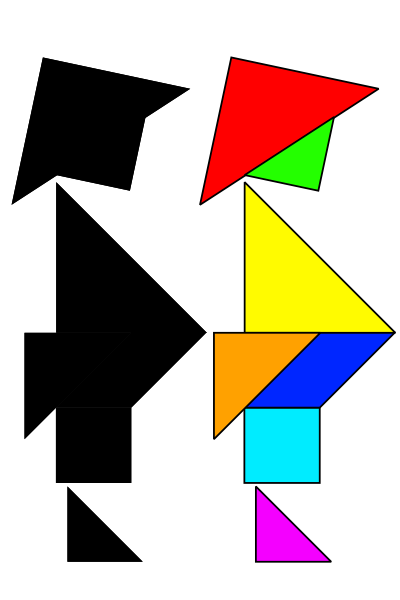
\includegraphics{tangram}
    \caption[]{An Example of Tangram.}
    \labfig{tangram}
\end{marginfigure}
Tangram is a Chinese puzzle game that has the objective of replicating a given silhouette with a set of 7 unique shapes.
All of these shapes have to be used and they may not overlay or be cut.
To solve the puzzle it is necessary to consider rather all parts together than a single part at a time.
Changing the position or rotation of one shape has consequences for all other shapes.\\
Quite similarly, the parameters of one brushstroke affects all nearby brushstrokes as well.
The fact that brushstrokes can overlap, have different colors and complex paths makes the matter even worse.

Thus, existing approaches are currently not capable of solving this complex task sufficiently.
\refch{ACV} presented many such methods which either aim at stylizing images or extracting brushstrokes.\\
Those which extract brushstrokes, are only capable of doing so for about half of all brushstrokes in a painting.
Such shortcomings are acceptable for further analysis, which prefers few accurate brushstrokes over many inaccurate ones.
However, it will not suffice for reconstructing the entire image.\\
Neural style transfer, which builds on filter-based approaches, is generally not suited for this problem.
Since a set of pixels is directly transformed into another set of pixels, there is no brushstroke data available.\\
Painterly renderings do not suffer from such problems.
They are inherently based on using brushstrokes to generate an entire image.
Most of these approaches focus on stylizing images, but few have tried to imitate paintings as well~\cite{paintbot,lpaintb}.\\
Both approaches trained recurrent neural networks specifically to reconstruct a single image.
The resulting approximations of paintings would resemble the original input, but not on a brushstroke level.
Even though they claim, that the trained neural network could be reused for style transfer, the use of a prediction network is likely a burden to the approach.
Ultimately, a set of parameters is sought and training a network to predict these parameters adds overhead in most scenarios.
Having such a network only really makes sense if it can be reused on many images.

This thesis will present an approach which is orthogonal to many recent implementations of drawings networks and painterly rendering.
Instead of training a network to predict the brushstroke parameters, the parameters are optimized directly.

Early painterly rendering approaches built on a similar set-up.
They would formulate an energy function to describe how well the parameters describe the image~\cite{hertzmann_review}.
Finding a minimum for these energy functions requires advanced searching algorithms like evolutionary algorithms~\cite{genetic_algo}.
\begin{marginfigure}
    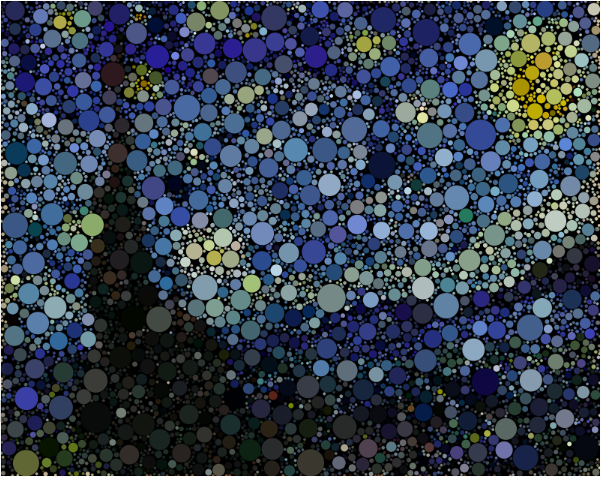
\includegraphics{genetic_starry_night}
    \caption[]{'The Starry Night' approximated by a genetic algorithm using only circles. \url{https://effyfan.com/2018/03/02/w6-van-gogh-flowfield/}}
    \labfig{genetic}
\end{marginfigure}
Albeit being capable of reconstructing images using pretty much any shape (also called unit), they have a major draw-back.
Such search algorithms are often inefficient since they are based on random sampling.
The sampling becomes even more inefficient if the number of degrees of freedom per unit is large, as it is the case for brushstrokes.

A solution to this problem is featured in many recently published approaches that use drawing networks.
Some reference \citeauthor*{worldmodel}'s idea of a world model~\cite{neuralpainters, learning2paint, strokenet} and present what is called a \textbf{neural renderer}.\\
Such a neural renderer makes the process of placing a brushstroke on canvas differentiable.
Thereby, a prediction network can learn easier compared to an approach without such a neural renderer.\\
Combining a differentiable renderer with a direct optimization-based approach would mitigate the inefficiency which other approaches suffered from.
Instead of randomly searching for minima, it would become possible to follow the gradient towards a minimum.
Thus, the approach of this thesis will consist of two components. \\
\begin{enumerate}
    \item A differentiable renderer which can generate images of brushstrokes from a parameter representation.
    \item An optimization procedure that iteratively approximates an image through brushstroke representations.
\end{enumerate}
Notably, \citeauthor*{gatys}'s approach to style transfer uses a similar set-up but optimizes pixels instead of brushstroke parameters.

The following two sections will present how each component of the approach has been realized.

%%%%%%%%%%%%%%%%%%%%%%%%%%%%%%%%%%%%%%%%%%%%%%%%%%%%%%%%%%%%%%%%%%%%%%%%%%%%%%%
%%%%%%%%%%%%%%%%%%% Neural Renderer %%%%%%%%%%%%%%%%%%%%%%%%%%%%%%%%%%%%%%%%%%%
%%%%%%%%%%%%%%%%%%%%%%%%%%%%%%%%%%%%%%%%%%%%%%%%%%%%%%%%%%%%%%%%%%%%%%%%%%%%%%%

\section{Neural Renderer}
\labsec{NeuralRend}

Generating brushstrokes artificially is a complex task.
There exist plenty of applications that are dedicated to this.
It is still possible to discern real brushstrokes from application-generated ones, even though some research is bridging this gap~\cite{wetbrush}.\\
It would be even harder to think of a differentiable way to generate brushstrokes from a set of parameters.

Neural networks solve this issue by finding a differentiable pipeline through training.
Previous works have shown that neural networks are capable of conditionally generating high-resolution and high-quality images and neural networks are inherently differentiable.
Therefore, it requires only data of brushstrokes and their parameters to train the network.\\
As previously stated, many already did so.
However, these approaches do not focus on the quality of the renderer.
Thus, they use simple painting applications like \citetitle{libmypaint} to generate the training data.
In this approach there shall be more emphasis on the render quality.

\subsection{Data Set}
\labsubsec{dataset}
There is no data sets openly available for this task
Therefore, a data set must be created explicitly for this approach, for which a painting tool (or something similar) has to be picked.\\
Three qualities are important when is comes to creating the data set:
\begin{enumerate}
    \item Suitable data format: As brushstrokes usually overlap in a painting, the data should already provide information about opacity or transparency, favorably in the common RGBA format.
    \item Data set size and variability: Only with enough different data points available, it will be possible to train a renderer reliably.
    \item Image quality: Brushstrokes should be as close to real-world brushstrokes as possible to ensure high-quality renderings.
\end{enumerate}
\marginnote{RGBA has a fourth channel besides the three color channels, which hold information about the opacity of every pixel.}

\subsubsection{Brushstroke Images}
There are some data sets with single scanned hand-drawn brushstrokes available on the internet~\cite{zolee_on_onlygfx}.
Some even come with the background removed on which they were drawn on.\\
Such data has the advantage that it consists of actual real-world brushstrokes.
On the other side, the data is very sparse.
Brushstrokes are very similar throughout the data set considering their path and color and come without any further information.
This would have the generator to interpolate data in the best case or not work for any unknown inputs in the worst case.\\
These limitations to the data make it unlikely that a generator could learn a coherent representation from it.

\subsubsection{Painting Libraries}
Painting libraries such as libmypaint are the de facto standard for neural renderer in drawing networks~\cite{neuralpainters, learning2paint, strokenet}.\\
They allow to fully control the output through parameters and thus make training for the renderer easier.
Still, this data falls short regarding the authenticity of rendered strokes, which are obviously computer generated.\\
This kind of data would allow to train a renderer, though it would likely cause the final images to look a bit ``flat''.

\subsubsection{Fluid Simulations}
Fluid simulations like those by \citeauthor*{wetbrush} give a better render quality compared to painting libraries. 
Unfortunately, only few implementations are openly available and if so are not as advanced.\\
\citeauthor*{SPIRAL} provide a fluid simulation package based on \citetitle{fluidpaint}~\cite{fluidpaint}.
It uses simple fluid dynamics to give artificial brushstrokes a more plastic look.
One problem, that comes with all simulations is that the brushstroke path not controlled directly, but by moving a virtual paintbrush.
Nevertheless, it is possible to partly account for this when creating the data set.\\
Another problem is the simulation time.
State-of-the-art approaches are just capable of rendering in real-time which is too slow for an entire data set.
Luckily, \citetitle{fluidpaint} is not as computationally expensive and can be parallelized to generate $100,000$ samples in about two hours.

All in all, \citetitle{fluidpaint} has been chosen as the tool to generate the data set.
The superior render quality justifies the additional work required to generate the data set.\\
There are other applications which are capable of simulating brushstrokes reasonably well like \citetitle{artrage}~\cite{artrage} and \citetitle{krita}~\cite{krita}.
Unfortunately, these application do not provide an interface to efficiently generate a data set.
\begin{marginfigure}
    \subfloat[Photograph]{%
        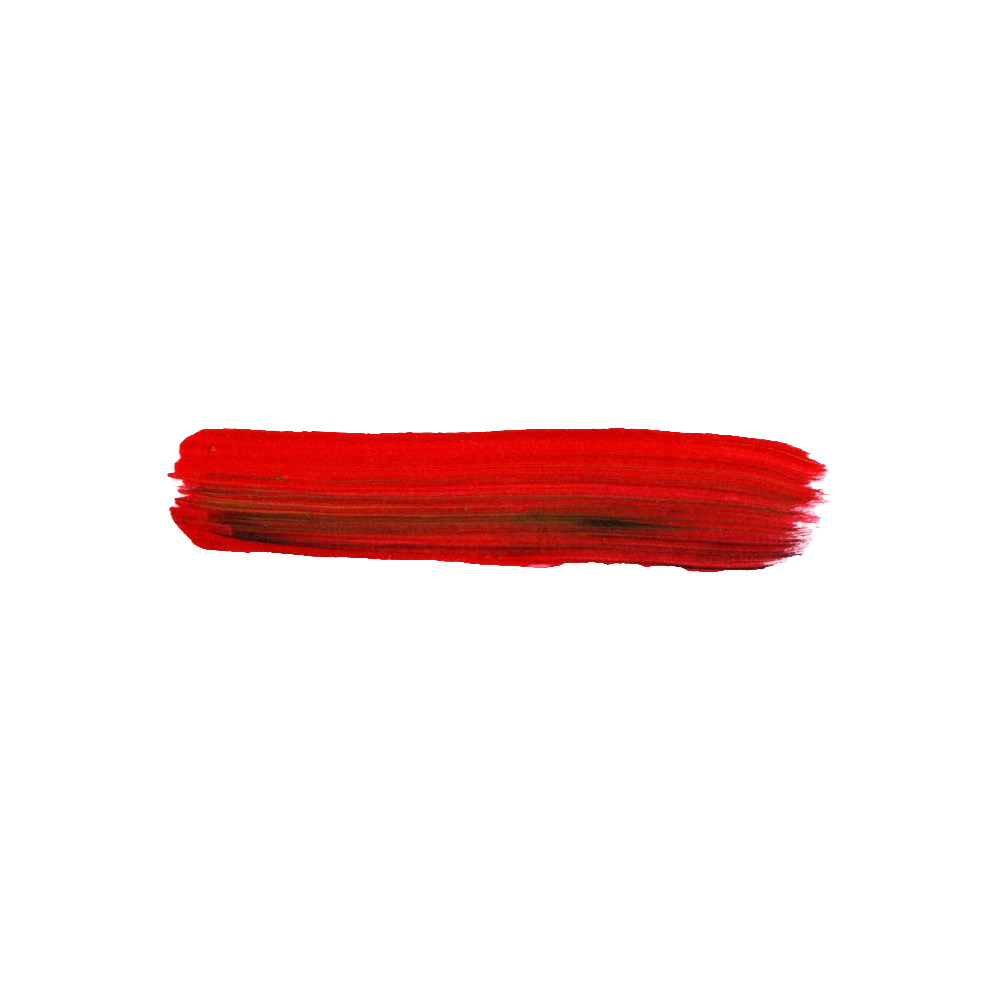
\includegraphics[width=.8\textwidth]{images/real_red_stroke}%
        \labfig{strokes:real}%
    }\qquad
    \subfloat[ArtRage]{%
        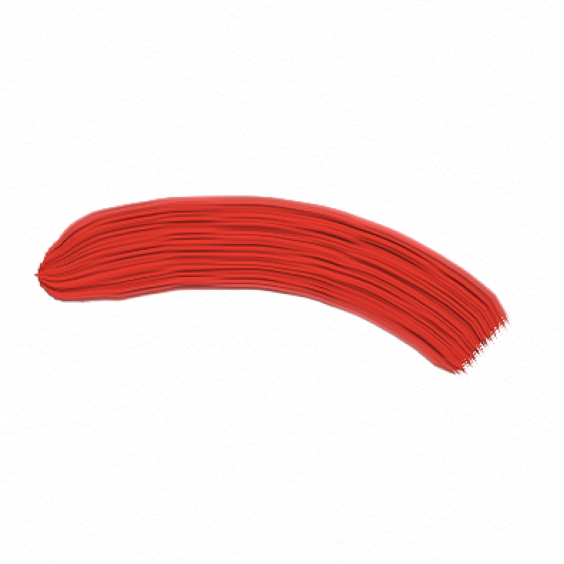
\includegraphics[width=.8\textwidth]{images/artrage_red_stroke}%
        \labfig{strokes:artrage}%
    }\qquad
    \subfloat[libmypaint]{%
        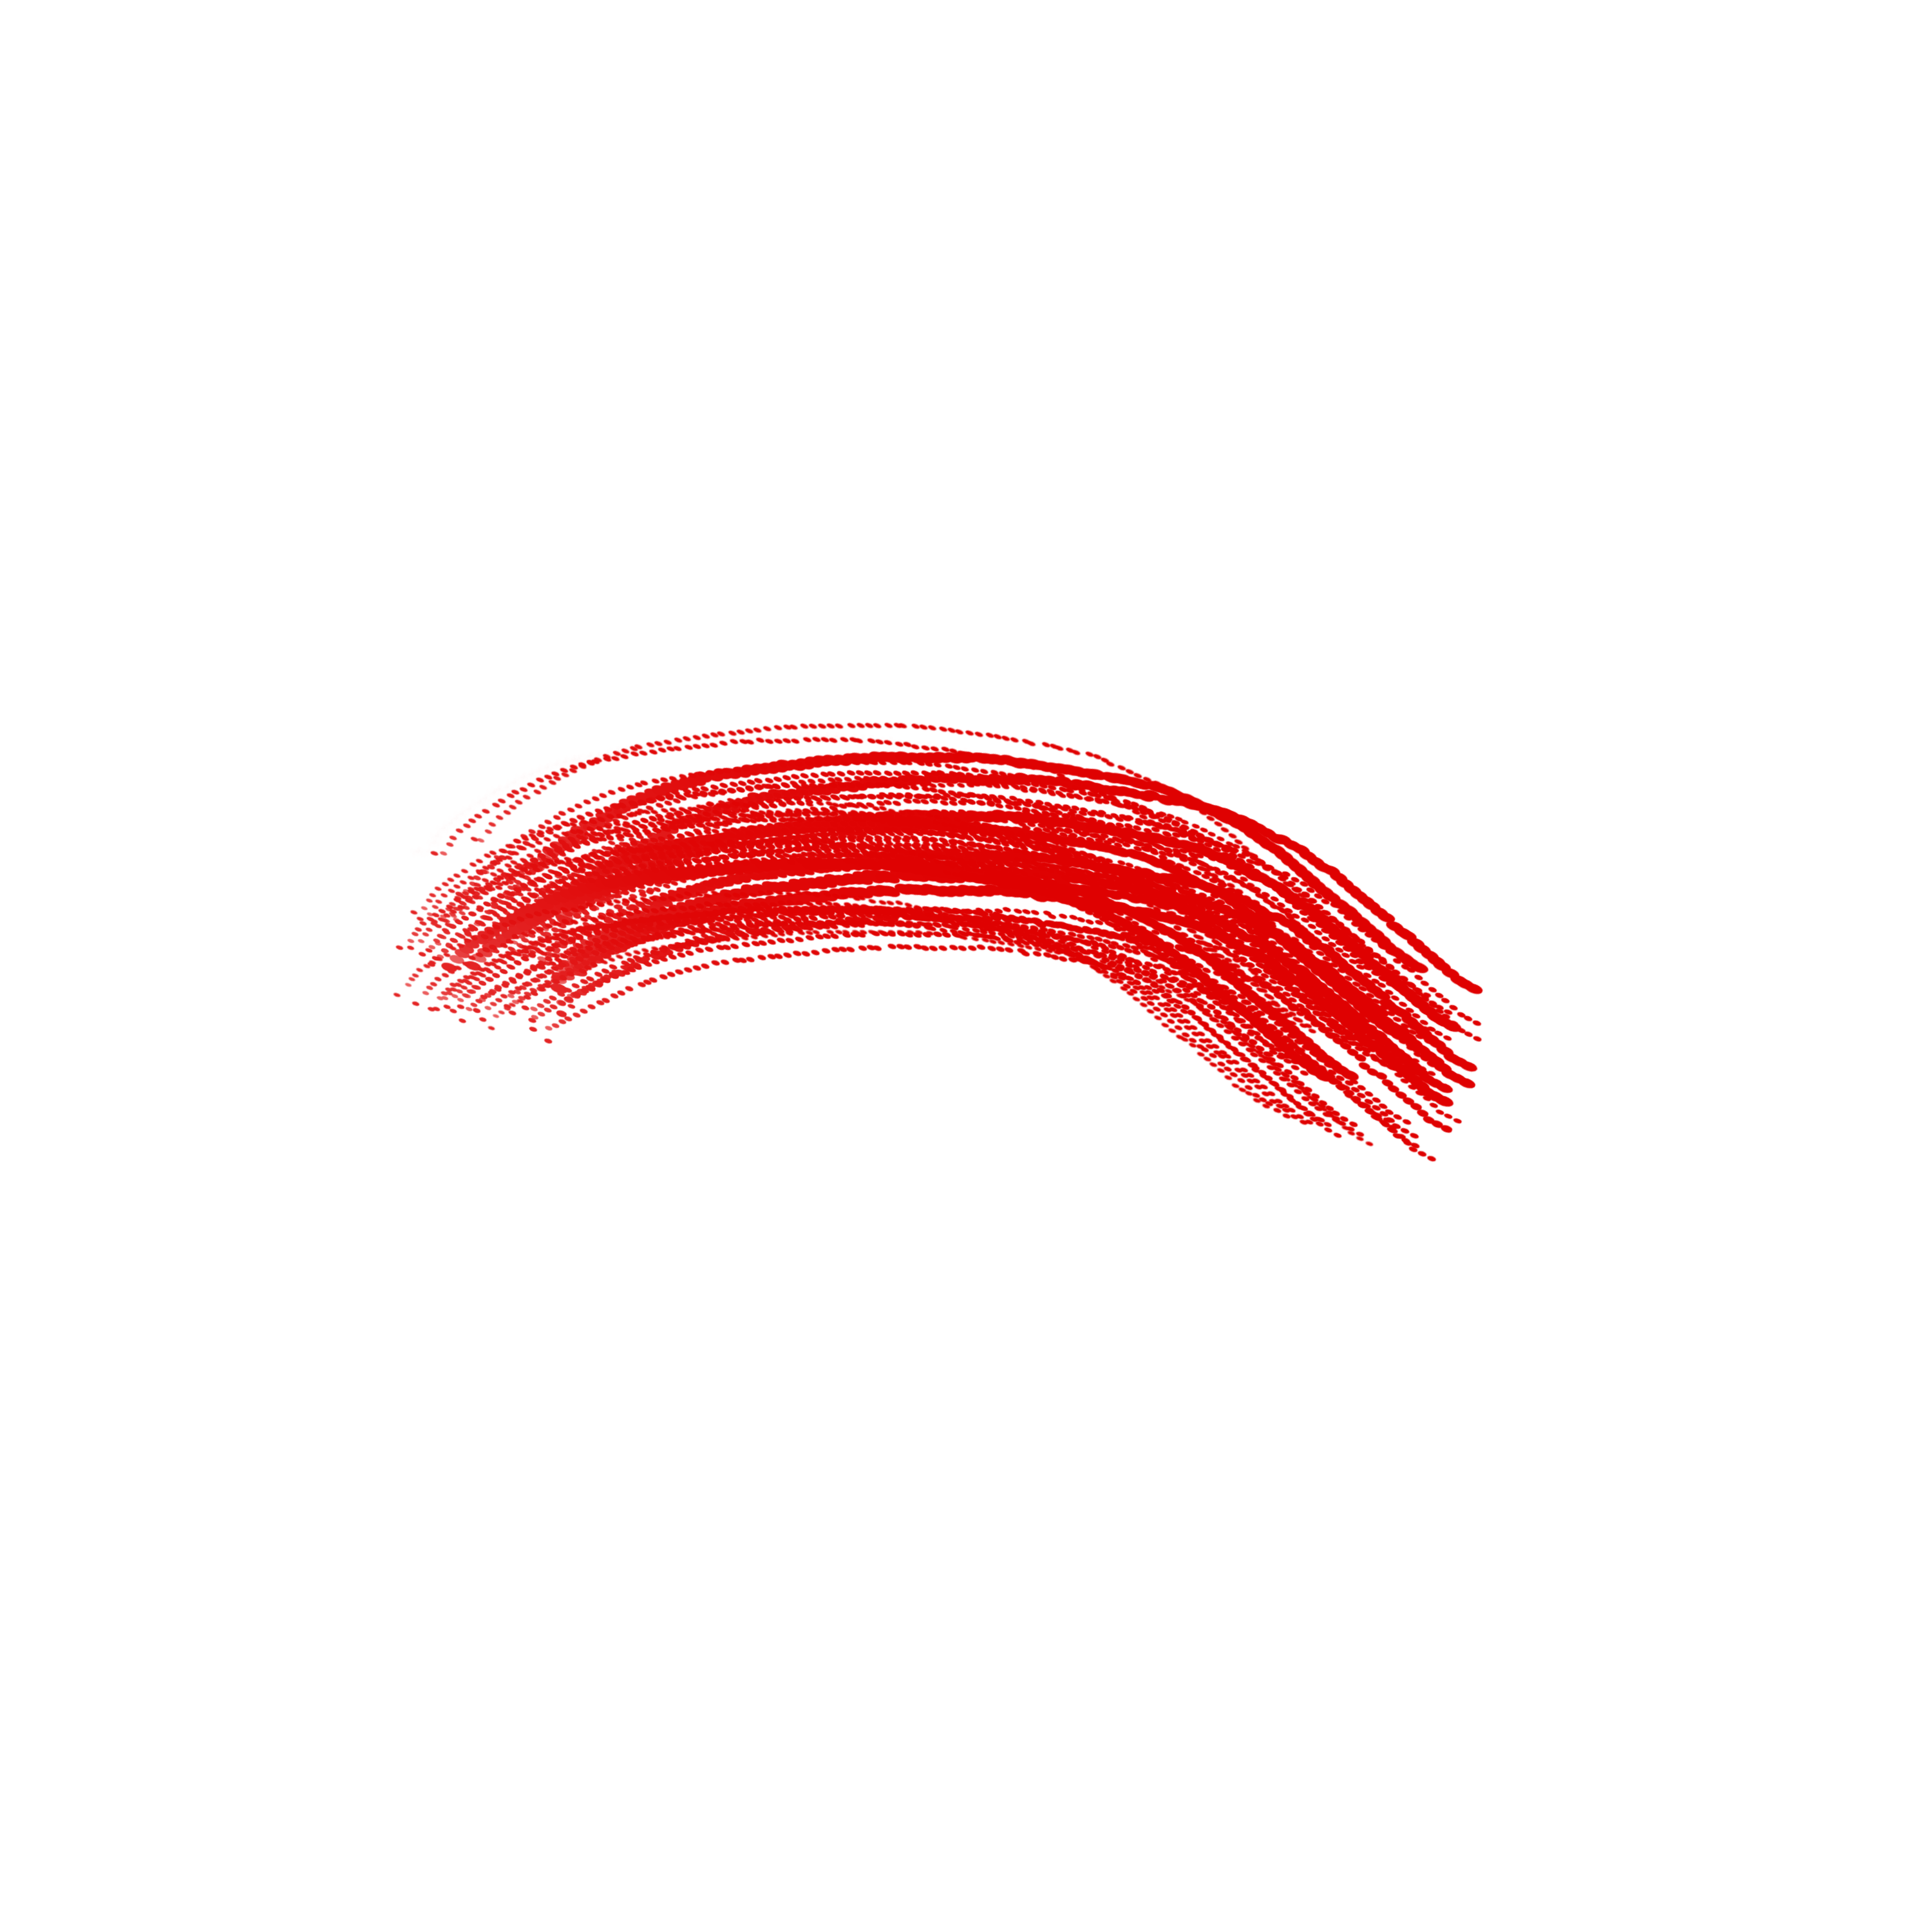
\includegraphics[width=.8\textwidth]{images/affinity_red_stroke}%
        \labfig{strokes:libmypaint}%
    }\qquad
    \subfloat[FluidPaint]{%
        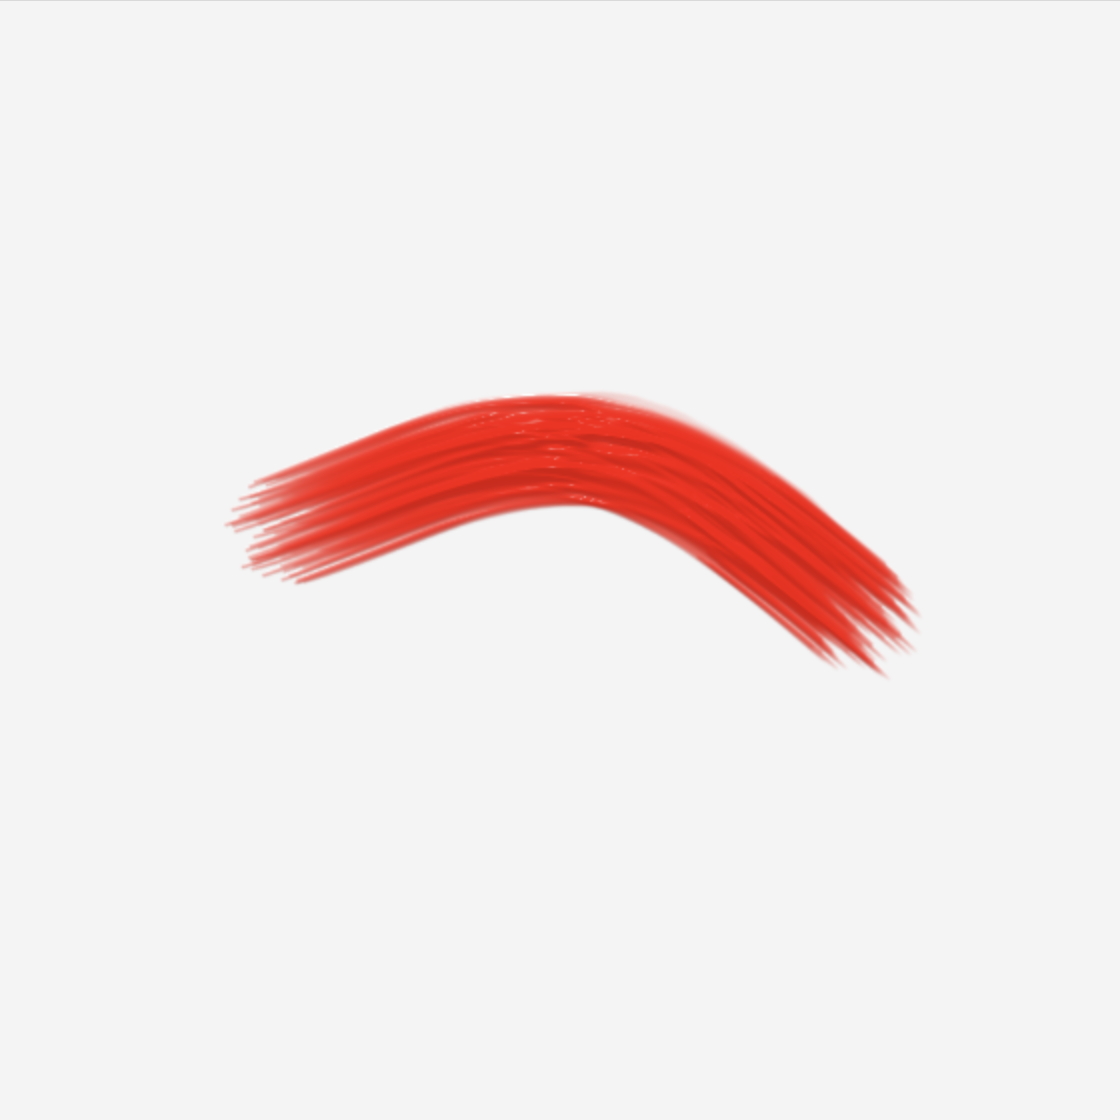
\includegraphics[width=.8\textwidth]{images/fluidpaint_red_stroke}%
        \labfig{strokes:fluidpaint}%
    }
    \caption[]{Comparison of similar brushstrokes in each data set}
    \labfig{strokes}
\end{marginfigure}

\subsubsection{Brushstroke Formalism}
The means of brushstroke production are now seized and what is left is to formulate the parameters that define a brushstrokes.
These parameters must quantify the following three properties of brushstrokes:
\begin{itemize}
    \item color
    \item thickness
    \item path
\end{itemize}









































The easiest of these three properties is quantifying the color.
Naturally, computer vision relies on the RGB format, which defines color as a set of three 8-Bit integer values between 0 and 255. 
As for path and thickness, these two properties depend on the given coordinate system.
FluidPaint represents the canvas as a 2D plane in the $[0, 1]$ range.
Thus, it makes sense to follow the same representation.

Thickness can be any value in $[0, 1]$  for each brushstroke, where 0 is an infinitely small brushstroke, and 1 is a brushstroke as wide as the canvas.
As both these edge cases do not make sense in this application, the range is constrained to $[.03, .2]$, which includes only brushstrokes that are visible and also do not cover the whole canvas.

Quantifying the path now is a little more tricky.
The fluid dynamics simulation that FluidPaint uses relies on internal time steps at which the equations are evaluated and subsequently rendered.
At the same time, each step allows only a linear motion of the brush handle between positions $a$ and $b$.
Subsequently, any curved paths must be split into linear/straight segments that together should resemble a curved line.
As more steps mean longer simulation times and fewer steps mean edgy movement, a value of 20 time-steps per stroke emerged as a good compromise \todo{this is actually different as the steps depend on the length of the path. Look this up}.
The same number of steps has been used in SPIRAL's implementation.

Another problem becomes how to express a curved path in numbers.
The most straightforward representation would be a sequence of points that make up any curved path.
Such an approach allows for the highest versatility, but at the same time introduces a noticeable amount of parameters as each point consists of 2 coordinates totaling to 40 values.
These values are also not independent of one another but should follow a reasonable path as otherwise, the resulting brushstroke would look somewhat like a random walk than an actual brushstroke.
Since works such as SPIRAL or 'Learning to Paint' face a quite similar obstacle, their solution should be applicable in this case as well.
Both used so-called 'Bezier curves' which parametrize curved paths by a limited set of numbers.
\begin{marginfigure}
    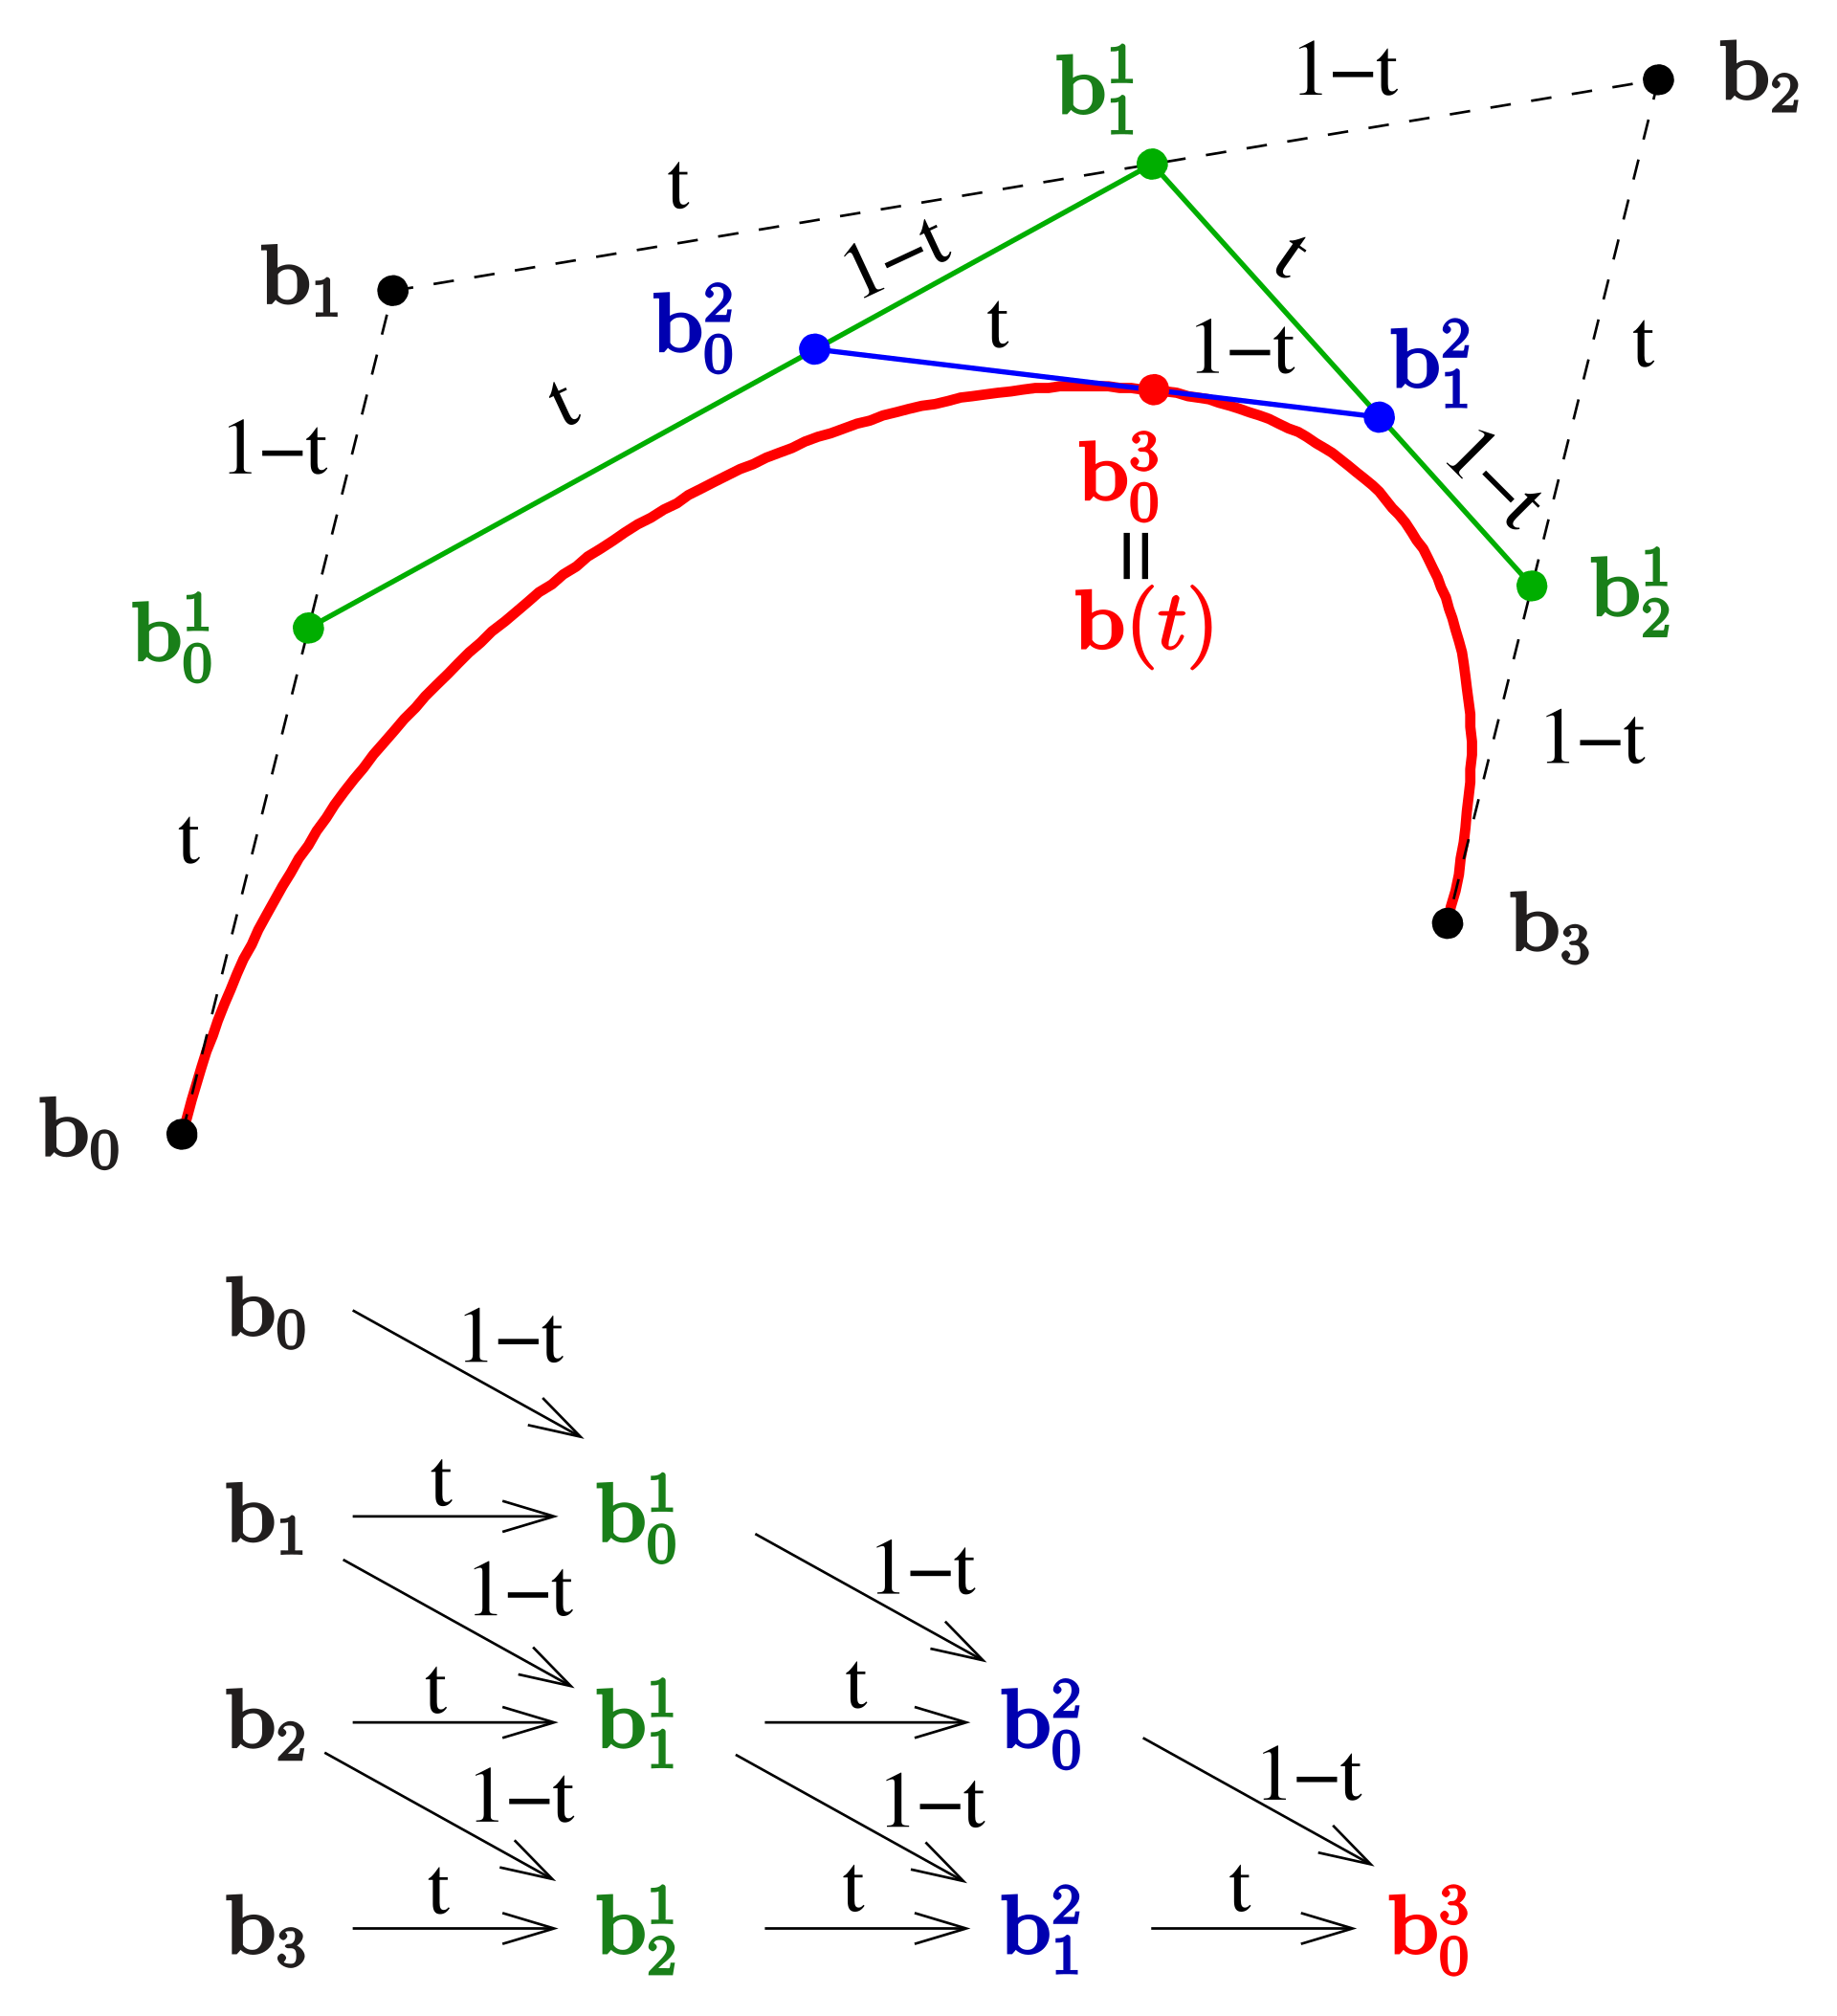
\includegraphics{bezier_sample}
    \caption[]{Sample of a 3rd degree Bezier curve, using the De-Casteljau-algorithm,
    \url{https:\/\/de.wikipedia.org\/wiki\/Bézierkurve\#\/media\/Datei:Bezier-cast-3.svg}}
    \labfig{genetic}
\end{marginfigure}

Bezier curves parametrize curved paths not as linear segments, but as analytical paths which can be used in computer models.
\todo{bezier curves margin note}
They can be of different orders, which allows them to follow more complicated paths.
In this case, the simplest form -- the first order Bezier curve-- is already sufficient.
It defines a curve through its start- and endpoint, as well as a control point.
The curve is then defined as the path of a point over the time interval $[0, T]$.
First, one connects the start- and endpoints with the control point to get two lines in return.
On these lines, lie two points that move linearly along their lines within a virtual time interval $[0, T]$.
Then these two points are connected in the same way as before by a third line.
Again, this line has a point moving along its path throughout $[0, T]$.
As the first two points that define the third line will move, the line's orientation will change as well, thus translating the linear movement of the point into a complex curved path.
The path that this point then takes in $[0, T]$ defines the Bezier curve.
A first-order Bezier curve will only bend into one direction or follow a straight path.
For higher orders, the displayed process can be applied iteratively and allows for more complex curves.
As brushstrokes usually follow a quite simple path and fewer parameters are preferred, Bezier curves of first-order are suitable as parametrization.

Ultimately, this gives ten values that are sufficient to parametrize brushstrokes with certain constraints:
\begin{itemize}
    \item Three 2D coordinates that define the Bezier curves (6 values).
    \item One thickness parameter.
    \item Three values in RGB space.
\end{itemize}


\subsubsection{Data Constraints}
\labsubsubsec{constraints}

Given the parameters listed in section \ref{sssec:formalism}, the data still needs further constraints to facilitate the generator's training even further.

Section \ref{sssec:fluidpaint} already hinted at the impracticality of online data generation.
A rough estimation by timing the rendering of 100.000 FluidPaint brushstrokes reveals that a dedicated CPU server is capable of generating 300 strokes per second.
\todo{experiment in appendix}
A neural network with batch size 32 is limited to $\approx 10$ iterations per second under these circumstances, which would mean a clear bottleneck.
Thus, it seems advisable to generate data beforehand with enough samples to cover the data space sufficiently.
It will allow for much faster access to data, as individual data samples are relatively small and can be stored in a binary data file such as HDF5.

Besides this constraint to the amount of data available, another set of constraints will be introduced to reduce the data space to 'valid' brushstrokes only.
'Valid' brushstrokes will be defined as brushstrokes that resemble real-world brushstrokes to a certain degree.
This primarily concerns two relations within a brushstroke:
\begin{itemize}
    \item Its width-to-length ratio.
    \item Its curvature.
\end{itemize}

The width-to-length ratio will be restricted to brushstrokes that are at least two times as long as they are wide.
\begin{equation}
\norm{\vec{s} - \vec{e}} \overset{!}{\leq}  2 \times (\text{brush size}) \labeq{bs}
\end{equation}
Due to the simulation background of FluidPaint shorter brushstrokes will show some artifacts due to the bristles' length in the simulation which depends on the width of the stroke.
Another reason for this is the intended use-case, which will focus on van Gogh paintings.
As van Gogh did not practice pointillism, most of his strokes have a length to them, which brings such a constraint in line with some characteristics of van Gogh's style.

The same argumentation applies to the curvature:
Most brushstrokes (especially those by van Gogh) have a certain 'flow' or 'smoothness' to them, which can be described by using strokes with large curvature radii and without any corners in the strokes' path.
Thus, the data set will also be restricted to strokes that follow these descriptions.
In order to achieve this with random sampling in mind, a multivariate Gaussian distribution is placed between start ($\vec{s}$) and end point ($\vec{e}$).
The two axes are rotated such that the short axis is in line with the vector
$\vec{a} = \vec{s} - \vec{e}$ while the other sits orthogonal.
Then both axes are scaled with $\norm{a}_2$ and also the handpicked values $\frac{1}{200}$ and $\frac{1}{25}$ for along $a$ and orthogonal to it, respectively.
Figure \ref{fig:datageneration} shows samples from this distribution for an exemplary brushstroke.
\begin{marginfigure}
    \resizebox{\textwidth}{!}{
        %% Creator: Matplotlib, PGF backend
%%
%% To include the figure in your LaTeX document, write
%%   \input{<filename>.pgf}
%%
%% Make sure the required packages are loaded in your preamble
%%   \usepackage{pgf}
%%
%% and, on pdftex
%%   \usepackage[utf8]{inputenc}\DeclareUnicodeCharacter{2212}{-}
%%
%% or, on luatex and xetex
%%   \usepackage{unicode-math}
%%
%% Figures using additional raster images can only be included by \input if
%% they are in the same directory as the main LaTeX file. For loading figures
%% from other directories you can use the `import` package
%%   \usepackage{import}
%%
%% and then include the figures with
%%   \import{<path to file>}{<filename>.pgf}
%%
%% Matplotlib used the following preamble
%%
\begingroup%
\makeatletter%
\begin{pgfpicture}%
\pgfpathrectangle{\pgfpointorigin}{\pgfqpoint{10.000000in}{10.000000in}}%
\pgfusepath{use as bounding box, clip}%
\begin{pgfscope}%
\pgfsetbuttcap%
\pgfsetmiterjoin%
\definecolor{currentfill}{rgb}{1.000000,1.000000,1.000000}%
\pgfsetfillcolor{currentfill}%
\pgfsetlinewidth{0.000000pt}%
\definecolor{currentstroke}{rgb}{1.000000,1.000000,1.000000}%
\pgfsetstrokecolor{currentstroke}%
\pgfsetdash{}{0pt}%
\pgfpathmoveto{\pgfqpoint{0.000000in}{0.000000in}}%
\pgfpathlineto{\pgfqpoint{10.000000in}{0.000000in}}%
\pgfpathlineto{\pgfqpoint{10.000000in}{10.000000in}}%
\pgfpathlineto{\pgfqpoint{0.000000in}{10.000000in}}%
\pgfpathclose%
\pgfusepath{fill}%
\end{pgfscope}%
\begin{pgfscope}%
\pgfsetbuttcap%
\pgfsetmiterjoin%
\definecolor{currentfill}{rgb}{1.000000,1.000000,1.000000}%
\pgfsetfillcolor{currentfill}%
\pgfsetlinewidth{0.000000pt}%
\definecolor{currentstroke}{rgb}{0.000000,0.000000,0.000000}%
\pgfsetstrokecolor{currentstroke}%
\pgfsetstrokeopacity{0.000000}%
\pgfsetdash{}{0pt}%
\pgfpathmoveto{\pgfqpoint{1.250000in}{1.100000in}}%
\pgfpathlineto{\pgfqpoint{9.000000in}{1.100000in}}%
\pgfpathlineto{\pgfqpoint{9.000000in}{8.800000in}}%
\pgfpathlineto{\pgfqpoint{1.250000in}{8.800000in}}%
\pgfpathclose%
\pgfusepath{fill}%
\end{pgfscope}%
\begin{pgfscope}%
\pgfpathrectangle{\pgfqpoint{1.250000in}{1.100000in}}{\pgfqpoint{7.750000in}{7.700000in}}%
\pgfusepath{clip}%
\pgfsetbuttcap%
\pgfsetroundjoin%
\definecolor{currentfill}{rgb}{0.121569,0.466667,0.705882}%
\pgfsetfillcolor{currentfill}%
\pgfsetlinewidth{1.003750pt}%
\definecolor{currentstroke}{rgb}{0.121569,0.466667,0.705882}%
\pgfsetstrokecolor{currentstroke}%
\pgfsetdash{}{0pt}%
\pgfsys@defobject{currentmarker}{\pgfqpoint{-0.041667in}{-0.041667in}}{\pgfqpoint{0.041667in}{0.041667in}}{%
\pgfpathmoveto{\pgfqpoint{0.000000in}{-0.041667in}}%
\pgfpathcurveto{\pgfqpoint{0.011050in}{-0.041667in}}{\pgfqpoint{0.021649in}{-0.037276in}}{\pgfqpoint{0.029463in}{-0.029463in}}%
\pgfpathcurveto{\pgfqpoint{0.037276in}{-0.021649in}}{\pgfqpoint{0.041667in}{-0.011050in}}{\pgfqpoint{0.041667in}{0.000000in}}%
\pgfpathcurveto{\pgfqpoint{0.041667in}{0.011050in}}{\pgfqpoint{0.037276in}{0.021649in}}{\pgfqpoint{0.029463in}{0.029463in}}%
\pgfpathcurveto{\pgfqpoint{0.021649in}{0.037276in}}{\pgfqpoint{0.011050in}{0.041667in}}{\pgfqpoint{0.000000in}{0.041667in}}%
\pgfpathcurveto{\pgfqpoint{-0.011050in}{0.041667in}}{\pgfqpoint{-0.021649in}{0.037276in}}{\pgfqpoint{-0.029463in}{0.029463in}}%
\pgfpathcurveto{\pgfqpoint{-0.037276in}{0.021649in}}{\pgfqpoint{-0.041667in}{0.011050in}}{\pgfqpoint{-0.041667in}{0.000000in}}%
\pgfpathcurveto{\pgfqpoint{-0.041667in}{-0.011050in}}{\pgfqpoint{-0.037276in}{-0.021649in}}{\pgfqpoint{-0.029463in}{-0.029463in}}%
\pgfpathcurveto{\pgfqpoint{-0.021649in}{-0.037276in}}{\pgfqpoint{-0.011050in}{-0.041667in}}{\pgfqpoint{0.000000in}{-0.041667in}}%
\pgfpathclose%
\pgfusepath{stroke,fill}%
}%
\begin{pgfscope}%
\pgfsys@transformshift{4.446296in}{4.944320in}%
\pgfsys@useobject{currentmarker}{}%
\end{pgfscope}%
\begin{pgfscope}%
\pgfsys@transformshift{4.648580in}{5.740066in}%
\pgfsys@useobject{currentmarker}{}%
\end{pgfscope}%
\begin{pgfscope}%
\pgfsys@transformshift{4.866971in}{5.235292in}%
\pgfsys@useobject{currentmarker}{}%
\end{pgfscope}%
\begin{pgfscope}%
\pgfsys@transformshift{4.976764in}{5.581239in}%
\pgfsys@useobject{currentmarker}{}%
\end{pgfscope}%
\begin{pgfscope}%
\pgfsys@transformshift{2.711341in}{2.763462in}%
\pgfsys@useobject{currentmarker}{}%
\end{pgfscope}%
\begin{pgfscope}%
\pgfsys@transformshift{4.062799in}{5.422729in}%
\pgfsys@useobject{currentmarker}{}%
\end{pgfscope}%
\begin{pgfscope}%
\pgfsys@transformshift{4.399868in}{7.045944in}%
\pgfsys@useobject{currentmarker}{}%
\end{pgfscope}%
\begin{pgfscope}%
\pgfsys@transformshift{4.455127in}{3.880766in}%
\pgfsys@useobject{currentmarker}{}%
\end{pgfscope}%
\begin{pgfscope}%
\pgfsys@transformshift{5.289763in}{6.313110in}%
\pgfsys@useobject{currentmarker}{}%
\end{pgfscope}%
\begin{pgfscope}%
\pgfsys@transformshift{5.974048in}{6.117658in}%
\pgfsys@useobject{currentmarker}{}%
\end{pgfscope}%
\begin{pgfscope}%
\pgfsys@transformshift{5.902568in}{5.653568in}%
\pgfsys@useobject{currentmarker}{}%
\end{pgfscope}%
\begin{pgfscope}%
\pgfsys@transformshift{5.167461in}{4.793771in}%
\pgfsys@useobject{currentmarker}{}%
\end{pgfscope}%
\begin{pgfscope}%
\pgfsys@transformshift{5.909388in}{6.533973in}%
\pgfsys@useobject{currentmarker}{}%
\end{pgfscope}%
\begin{pgfscope}%
\pgfsys@transformshift{5.093612in}{5.137085in}%
\pgfsys@useobject{currentmarker}{}%
\end{pgfscope}%
\begin{pgfscope}%
\pgfsys@transformshift{3.299058in}{2.085167in}%
\pgfsys@useobject{currentmarker}{}%
\end{pgfscope}%
\begin{pgfscope}%
\pgfsys@transformshift{4.956854in}{5.825046in}%
\pgfsys@useobject{currentmarker}{}%
\end{pgfscope}%
\begin{pgfscope}%
\pgfsys@transformshift{4.390762in}{4.618962in}%
\pgfsys@useobject{currentmarker}{}%
\end{pgfscope}%
\begin{pgfscope}%
\pgfsys@transformshift{5.649067in}{7.519862in}%
\pgfsys@useobject{currentmarker}{}%
\end{pgfscope}%
\begin{pgfscope}%
\pgfsys@transformshift{5.090611in}{6.156232in}%
\pgfsys@useobject{currentmarker}{}%
\end{pgfscope}%
\begin{pgfscope}%
\pgfsys@transformshift{3.990133in}{4.438412in}%
\pgfsys@useobject{currentmarker}{}%
\end{pgfscope}%
\begin{pgfscope}%
\pgfsys@transformshift{4.318809in}{5.055863in}%
\pgfsys@useobject{currentmarker}{}%
\end{pgfscope}%
\begin{pgfscope}%
\pgfsys@transformshift{4.339208in}{3.853755in}%
\pgfsys@useobject{currentmarker}{}%
\end{pgfscope}%
\begin{pgfscope}%
\pgfsys@transformshift{6.082365in}{6.539471in}%
\pgfsys@useobject{currentmarker}{}%
\end{pgfscope}%
\begin{pgfscope}%
\pgfsys@transformshift{5.234880in}{5.335681in}%
\pgfsys@useobject{currentmarker}{}%
\end{pgfscope}%
\begin{pgfscope}%
\pgfsys@transformshift{4.068883in}{3.677030in}%
\pgfsys@useobject{currentmarker}{}%
\end{pgfscope}%
\begin{pgfscope}%
\pgfsys@transformshift{3.905556in}{4.222566in}%
\pgfsys@useobject{currentmarker}{}%
\end{pgfscope}%
\begin{pgfscope}%
\pgfsys@transformshift{5.393184in}{7.540256in}%
\pgfsys@useobject{currentmarker}{}%
\end{pgfscope}%
\begin{pgfscope}%
\pgfsys@transformshift{5.545587in}{5.851532in}%
\pgfsys@useobject{currentmarker}{}%
\end{pgfscope}%
\begin{pgfscope}%
\pgfsys@transformshift{4.226134in}{5.368741in}%
\pgfsys@useobject{currentmarker}{}%
\end{pgfscope}%
\begin{pgfscope}%
\pgfsys@transformshift{5.905595in}{6.170528in}%
\pgfsys@useobject{currentmarker}{}%
\end{pgfscope}%
\begin{pgfscope}%
\pgfsys@transformshift{4.521417in}{4.070533in}%
\pgfsys@useobject{currentmarker}{}%
\end{pgfscope}%
\begin{pgfscope}%
\pgfsys@transformshift{5.025554in}{5.309027in}%
\pgfsys@useobject{currentmarker}{}%
\end{pgfscope}%
\begin{pgfscope}%
\pgfsys@transformshift{3.744836in}{4.453472in}%
\pgfsys@useobject{currentmarker}{}%
\end{pgfscope}%
\begin{pgfscope}%
\pgfsys@transformshift{5.233583in}{6.072771in}%
\pgfsys@useobject{currentmarker}{}%
\end{pgfscope}%
\begin{pgfscope}%
\pgfsys@transformshift{4.183227in}{5.943304in}%
\pgfsys@useobject{currentmarker}{}%
\end{pgfscope}%
\begin{pgfscope}%
\pgfsys@transformshift{3.936834in}{3.552480in}%
\pgfsys@useobject{currentmarker}{}%
\end{pgfscope}%
\begin{pgfscope}%
\pgfsys@transformshift{4.434789in}{5.417619in}%
\pgfsys@useobject{currentmarker}{}%
\end{pgfscope}%
\begin{pgfscope}%
\pgfsys@transformshift{5.631918in}{4.541621in}%
\pgfsys@useobject{currentmarker}{}%
\end{pgfscope}%
\begin{pgfscope}%
\pgfsys@transformshift{3.379850in}{2.518338in}%
\pgfsys@useobject{currentmarker}{}%
\end{pgfscope}%
\begin{pgfscope}%
\pgfsys@transformshift{4.640462in}{6.351390in}%
\pgfsys@useobject{currentmarker}{}%
\end{pgfscope}%
\begin{pgfscope}%
\pgfsys@transformshift{5.588589in}{6.191089in}%
\pgfsys@useobject{currentmarker}{}%
\end{pgfscope}%
\begin{pgfscope}%
\pgfsys@transformshift{4.806000in}{5.640478in}%
\pgfsys@useobject{currentmarker}{}%
\end{pgfscope}%
\begin{pgfscope}%
\pgfsys@transformshift{5.233215in}{6.565680in}%
\pgfsys@useobject{currentmarker}{}%
\end{pgfscope}%
\begin{pgfscope}%
\pgfsys@transformshift{5.414218in}{4.418051in}%
\pgfsys@useobject{currentmarker}{}%
\end{pgfscope}%
\begin{pgfscope}%
\pgfsys@transformshift{4.627407in}{5.446321in}%
\pgfsys@useobject{currentmarker}{}%
\end{pgfscope}%
\begin{pgfscope}%
\pgfsys@transformshift{5.863884in}{6.630180in}%
\pgfsys@useobject{currentmarker}{}%
\end{pgfscope}%
\begin{pgfscope}%
\pgfsys@transformshift{4.489137in}{3.438186in}%
\pgfsys@useobject{currentmarker}{}%
\end{pgfscope}%
\begin{pgfscope}%
\pgfsys@transformshift{4.934354in}{5.308510in}%
\pgfsys@useobject{currentmarker}{}%
\end{pgfscope}%
\begin{pgfscope}%
\pgfsys@transformshift{4.257096in}{3.073789in}%
\pgfsys@useobject{currentmarker}{}%
\end{pgfscope}%
\begin{pgfscope}%
\pgfsys@transformshift{4.283839in}{5.704227in}%
\pgfsys@useobject{currentmarker}{}%
\end{pgfscope}%
\begin{pgfscope}%
\pgfsys@transformshift{5.789807in}{5.885701in}%
\pgfsys@useobject{currentmarker}{}%
\end{pgfscope}%
\begin{pgfscope}%
\pgfsys@transformshift{4.897169in}{4.085618in}%
\pgfsys@useobject{currentmarker}{}%
\end{pgfscope}%
\begin{pgfscope}%
\pgfsys@transformshift{6.225840in}{5.494487in}%
\pgfsys@useobject{currentmarker}{}%
\end{pgfscope}%
\begin{pgfscope}%
\pgfsys@transformshift{4.346013in}{5.542624in}%
\pgfsys@useobject{currentmarker}{}%
\end{pgfscope}%
\begin{pgfscope}%
\pgfsys@transformshift{4.724132in}{6.166122in}%
\pgfsys@useobject{currentmarker}{}%
\end{pgfscope}%
\begin{pgfscope}%
\pgfsys@transformshift{5.705120in}{6.054509in}%
\pgfsys@useobject{currentmarker}{}%
\end{pgfscope}%
\begin{pgfscope}%
\pgfsys@transformshift{4.740475in}{3.944492in}%
\pgfsys@useobject{currentmarker}{}%
\end{pgfscope}%
\begin{pgfscope}%
\pgfsys@transformshift{4.618355in}{4.869041in}%
\pgfsys@useobject{currentmarker}{}%
\end{pgfscope}%
\begin{pgfscope}%
\pgfsys@transformshift{3.215908in}{3.752179in}%
\pgfsys@useobject{currentmarker}{}%
\end{pgfscope}%
\begin{pgfscope}%
\pgfsys@transformshift{5.771356in}{4.867109in}%
\pgfsys@useobject{currentmarker}{}%
\end{pgfscope}%
\begin{pgfscope}%
\pgfsys@transformshift{4.826082in}{4.187374in}%
\pgfsys@useobject{currentmarker}{}%
\end{pgfscope}%
\begin{pgfscope}%
\pgfsys@transformshift{4.486963in}{4.486378in}%
\pgfsys@useobject{currentmarker}{}%
\end{pgfscope}%
\begin{pgfscope}%
\pgfsys@transformshift{4.863197in}{4.596623in}%
\pgfsys@useobject{currentmarker}{}%
\end{pgfscope}%
\begin{pgfscope}%
\pgfsys@transformshift{3.578844in}{3.242194in}%
\pgfsys@useobject{currentmarker}{}%
\end{pgfscope}%
\begin{pgfscope}%
\pgfsys@transformshift{4.244939in}{5.410042in}%
\pgfsys@useobject{currentmarker}{}%
\end{pgfscope}%
\begin{pgfscope}%
\pgfsys@transformshift{3.988812in}{4.577346in}%
\pgfsys@useobject{currentmarker}{}%
\end{pgfscope}%
\begin{pgfscope}%
\pgfsys@transformshift{4.402675in}{4.151624in}%
\pgfsys@useobject{currentmarker}{}%
\end{pgfscope}%
\begin{pgfscope}%
\pgfsys@transformshift{5.338998in}{5.300106in}%
\pgfsys@useobject{currentmarker}{}%
\end{pgfscope}%
\begin{pgfscope}%
\pgfsys@transformshift{6.540993in}{6.996707in}%
\pgfsys@useobject{currentmarker}{}%
\end{pgfscope}%
\begin{pgfscope}%
\pgfsys@transformshift{4.476051in}{5.368132in}%
\pgfsys@useobject{currentmarker}{}%
\end{pgfscope}%
\begin{pgfscope}%
\pgfsys@transformshift{3.870034in}{4.570308in}%
\pgfsys@useobject{currentmarker}{}%
\end{pgfscope}%
\begin{pgfscope}%
\pgfsys@transformshift{3.884930in}{4.094946in}%
\pgfsys@useobject{currentmarker}{}%
\end{pgfscope}%
\begin{pgfscope}%
\pgfsys@transformshift{5.658652in}{5.702464in}%
\pgfsys@useobject{currentmarker}{}%
\end{pgfscope}%
\begin{pgfscope}%
\pgfsys@transformshift{5.528402in}{5.895155in}%
\pgfsys@useobject{currentmarker}{}%
\end{pgfscope}%
\begin{pgfscope}%
\pgfsys@transformshift{4.877423in}{5.204343in}%
\pgfsys@useobject{currentmarker}{}%
\end{pgfscope}%
\begin{pgfscope}%
\pgfsys@transformshift{4.271464in}{5.775369in}%
\pgfsys@useobject{currentmarker}{}%
\end{pgfscope}%
\begin{pgfscope}%
\pgfsys@transformshift{4.576727in}{4.880689in}%
\pgfsys@useobject{currentmarker}{}%
\end{pgfscope}%
\begin{pgfscope}%
\pgfsys@transformshift{5.219880in}{6.732183in}%
\pgfsys@useobject{currentmarker}{}%
\end{pgfscope}%
\begin{pgfscope}%
\pgfsys@transformshift{5.150752in}{4.617526in}%
\pgfsys@useobject{currentmarker}{}%
\end{pgfscope}%
\begin{pgfscope}%
\pgfsys@transformshift{3.510915in}{4.878002in}%
\pgfsys@useobject{currentmarker}{}%
\end{pgfscope}%
\begin{pgfscope}%
\pgfsys@transformshift{3.842448in}{3.183670in}%
\pgfsys@useobject{currentmarker}{}%
\end{pgfscope}%
\begin{pgfscope}%
\pgfsys@transformshift{4.288504in}{2.451504in}%
\pgfsys@useobject{currentmarker}{}%
\end{pgfscope}%
\begin{pgfscope}%
\pgfsys@transformshift{5.029615in}{5.975821in}%
\pgfsys@useobject{currentmarker}{}%
\end{pgfscope}%
\begin{pgfscope}%
\pgfsys@transformshift{5.299296in}{6.409234in}%
\pgfsys@useobject{currentmarker}{}%
\end{pgfscope}%
\begin{pgfscope}%
\pgfsys@transformshift{5.029067in}{5.513894in}%
\pgfsys@useobject{currentmarker}{}%
\end{pgfscope}%
\begin{pgfscope}%
\pgfsys@transformshift{5.017564in}{5.852829in}%
\pgfsys@useobject{currentmarker}{}%
\end{pgfscope}%
\begin{pgfscope}%
\pgfsys@transformshift{4.159967in}{4.124760in}%
\pgfsys@useobject{currentmarker}{}%
\end{pgfscope}%
\begin{pgfscope}%
\pgfsys@transformshift{4.396211in}{4.944367in}%
\pgfsys@useobject{currentmarker}{}%
\end{pgfscope}%
\begin{pgfscope}%
\pgfsys@transformshift{5.303507in}{5.645807in}%
\pgfsys@useobject{currentmarker}{}%
\end{pgfscope}%
\begin{pgfscope}%
\pgfsys@transformshift{3.913543in}{4.589413in}%
\pgfsys@useobject{currentmarker}{}%
\end{pgfscope}%
\begin{pgfscope}%
\pgfsys@transformshift{4.022979in}{4.437472in}%
\pgfsys@useobject{currentmarker}{}%
\end{pgfscope}%
\begin{pgfscope}%
\pgfsys@transformshift{4.015933in}{3.949540in}%
\pgfsys@useobject{currentmarker}{}%
\end{pgfscope}%
\begin{pgfscope}%
\pgfsys@transformshift{4.616392in}{4.329131in}%
\pgfsys@useobject{currentmarker}{}%
\end{pgfscope}%
\begin{pgfscope}%
\pgfsys@transformshift{4.608554in}{4.269079in}%
\pgfsys@useobject{currentmarker}{}%
\end{pgfscope}%
\begin{pgfscope}%
\pgfsys@transformshift{4.342717in}{3.339463in}%
\pgfsys@useobject{currentmarker}{}%
\end{pgfscope}%
\begin{pgfscope}%
\pgfsys@transformshift{6.365832in}{7.316184in}%
\pgfsys@useobject{currentmarker}{}%
\end{pgfscope}%
\begin{pgfscope}%
\pgfsys@transformshift{4.482550in}{5.620129in}%
\pgfsys@useobject{currentmarker}{}%
\end{pgfscope}%
\begin{pgfscope}%
\pgfsys@transformshift{5.267756in}{5.180839in}%
\pgfsys@useobject{currentmarker}{}%
\end{pgfscope}%
\begin{pgfscope}%
\pgfsys@transformshift{7.089923in}{6.674228in}%
\pgfsys@useobject{currentmarker}{}%
\end{pgfscope}%
\begin{pgfscope}%
\pgfsys@transformshift{6.900530in}{6.801608in}%
\pgfsys@useobject{currentmarker}{}%
\end{pgfscope}%
\begin{pgfscope}%
\pgfsys@transformshift{5.347021in}{4.149752in}%
\pgfsys@useobject{currentmarker}{}%
\end{pgfscope}%
\begin{pgfscope}%
\pgfsys@transformshift{4.843429in}{4.236180in}%
\pgfsys@useobject{currentmarker}{}%
\end{pgfscope}%
\begin{pgfscope}%
\pgfsys@transformshift{4.923480in}{6.105906in}%
\pgfsys@useobject{currentmarker}{}%
\end{pgfscope}%
\begin{pgfscope}%
\pgfsys@transformshift{4.152221in}{4.038332in}%
\pgfsys@useobject{currentmarker}{}%
\end{pgfscope}%
\begin{pgfscope}%
\pgfsys@transformshift{5.420370in}{5.351259in}%
\pgfsys@useobject{currentmarker}{}%
\end{pgfscope}%
\begin{pgfscope}%
\pgfsys@transformshift{5.373985in}{5.786243in}%
\pgfsys@useobject{currentmarker}{}%
\end{pgfscope}%
\begin{pgfscope}%
\pgfsys@transformshift{4.486549in}{4.054694in}%
\pgfsys@useobject{currentmarker}{}%
\end{pgfscope}%
\begin{pgfscope}%
\pgfsys@transformshift{5.176141in}{5.904152in}%
\pgfsys@useobject{currentmarker}{}%
\end{pgfscope}%
\begin{pgfscope}%
\pgfsys@transformshift{5.220442in}{4.391660in}%
\pgfsys@useobject{currentmarker}{}%
\end{pgfscope}%
\begin{pgfscope}%
\pgfsys@transformshift{5.162986in}{4.797005in}%
\pgfsys@useobject{currentmarker}{}%
\end{pgfscope}%
\begin{pgfscope}%
\pgfsys@transformshift{4.487208in}{4.006776in}%
\pgfsys@useobject{currentmarker}{}%
\end{pgfscope}%
\begin{pgfscope}%
\pgfsys@transformshift{4.453460in}{5.438436in}%
\pgfsys@useobject{currentmarker}{}%
\end{pgfscope}%
\begin{pgfscope}%
\pgfsys@transformshift{5.333393in}{4.892651in}%
\pgfsys@useobject{currentmarker}{}%
\end{pgfscope}%
\begin{pgfscope}%
\pgfsys@transformshift{5.131587in}{5.753069in}%
\pgfsys@useobject{currentmarker}{}%
\end{pgfscope}%
\begin{pgfscope}%
\pgfsys@transformshift{4.067118in}{4.207749in}%
\pgfsys@useobject{currentmarker}{}%
\end{pgfscope}%
\begin{pgfscope}%
\pgfsys@transformshift{5.139581in}{7.336066in}%
\pgfsys@useobject{currentmarker}{}%
\end{pgfscope}%
\begin{pgfscope}%
\pgfsys@transformshift{4.256863in}{4.581942in}%
\pgfsys@useobject{currentmarker}{}%
\end{pgfscope}%
\begin{pgfscope}%
\pgfsys@transformshift{5.010763in}{5.381262in}%
\pgfsys@useobject{currentmarker}{}%
\end{pgfscope}%
\begin{pgfscope}%
\pgfsys@transformshift{4.694127in}{5.546835in}%
\pgfsys@useobject{currentmarker}{}%
\end{pgfscope}%
\begin{pgfscope}%
\pgfsys@transformshift{4.083350in}{3.708123in}%
\pgfsys@useobject{currentmarker}{}%
\end{pgfscope}%
\begin{pgfscope}%
\pgfsys@transformshift{4.933473in}{6.025027in}%
\pgfsys@useobject{currentmarker}{}%
\end{pgfscope}%
\begin{pgfscope}%
\pgfsys@transformshift{4.986989in}{6.264224in}%
\pgfsys@useobject{currentmarker}{}%
\end{pgfscope}%
\begin{pgfscope}%
\pgfsys@transformshift{4.574033in}{3.930627in}%
\pgfsys@useobject{currentmarker}{}%
\end{pgfscope}%
\begin{pgfscope}%
\pgfsys@transformshift{4.314617in}{4.352286in}%
\pgfsys@useobject{currentmarker}{}%
\end{pgfscope}%
\begin{pgfscope}%
\pgfsys@transformshift{4.452060in}{4.762707in}%
\pgfsys@useobject{currentmarker}{}%
\end{pgfscope}%
\begin{pgfscope}%
\pgfsys@transformshift{2.897741in}{1.940296in}%
\pgfsys@useobject{currentmarker}{}%
\end{pgfscope}%
\begin{pgfscope}%
\pgfsys@transformshift{5.969306in}{6.241054in}%
\pgfsys@useobject{currentmarker}{}%
\end{pgfscope}%
\begin{pgfscope}%
\pgfsys@transformshift{4.110203in}{4.311365in}%
\pgfsys@useobject{currentmarker}{}%
\end{pgfscope}%
\begin{pgfscope}%
\pgfsys@transformshift{5.590385in}{5.346903in}%
\pgfsys@useobject{currentmarker}{}%
\end{pgfscope}%
\begin{pgfscope}%
\pgfsys@transformshift{5.023482in}{3.810667in}%
\pgfsys@useobject{currentmarker}{}%
\end{pgfscope}%
\begin{pgfscope}%
\pgfsys@transformshift{4.736659in}{5.618624in}%
\pgfsys@useobject{currentmarker}{}%
\end{pgfscope}%
\begin{pgfscope}%
\pgfsys@transformshift{6.211443in}{6.371800in}%
\pgfsys@useobject{currentmarker}{}%
\end{pgfscope}%
\begin{pgfscope}%
\pgfsys@transformshift{3.893491in}{3.858327in}%
\pgfsys@useobject{currentmarker}{}%
\end{pgfscope}%
\begin{pgfscope}%
\pgfsys@transformshift{3.835989in}{3.430939in}%
\pgfsys@useobject{currentmarker}{}%
\end{pgfscope}%
\begin{pgfscope}%
\pgfsys@transformshift{4.373373in}{6.096262in}%
\pgfsys@useobject{currentmarker}{}%
\end{pgfscope}%
\begin{pgfscope}%
\pgfsys@transformshift{5.806748in}{6.667064in}%
\pgfsys@useobject{currentmarker}{}%
\end{pgfscope}%
\begin{pgfscope}%
\pgfsys@transformshift{5.132971in}{4.953034in}%
\pgfsys@useobject{currentmarker}{}%
\end{pgfscope}%
\begin{pgfscope}%
\pgfsys@transformshift{5.442190in}{7.593894in}%
\pgfsys@useobject{currentmarker}{}%
\end{pgfscope}%
\begin{pgfscope}%
\pgfsys@transformshift{5.132319in}{4.281671in}%
\pgfsys@useobject{currentmarker}{}%
\end{pgfscope}%
\begin{pgfscope}%
\pgfsys@transformshift{3.806985in}{3.662878in}%
\pgfsys@useobject{currentmarker}{}%
\end{pgfscope}%
\begin{pgfscope}%
\pgfsys@transformshift{5.271534in}{5.893118in}%
\pgfsys@useobject{currentmarker}{}%
\end{pgfscope}%
\begin{pgfscope}%
\pgfsys@transformshift{5.664543in}{5.730086in}%
\pgfsys@useobject{currentmarker}{}%
\end{pgfscope}%
\begin{pgfscope}%
\pgfsys@transformshift{4.699306in}{3.240430in}%
\pgfsys@useobject{currentmarker}{}%
\end{pgfscope}%
\begin{pgfscope}%
\pgfsys@transformshift{5.218206in}{5.216500in}%
\pgfsys@useobject{currentmarker}{}%
\end{pgfscope}%
\begin{pgfscope}%
\pgfsys@transformshift{4.001939in}{4.378296in}%
\pgfsys@useobject{currentmarker}{}%
\end{pgfscope}%
\begin{pgfscope}%
\pgfsys@transformshift{5.075482in}{7.257422in}%
\pgfsys@useobject{currentmarker}{}%
\end{pgfscope}%
\begin{pgfscope}%
\pgfsys@transformshift{3.905182in}{3.267347in}%
\pgfsys@useobject{currentmarker}{}%
\end{pgfscope}%
\begin{pgfscope}%
\pgfsys@transformshift{4.712840in}{4.769005in}%
\pgfsys@useobject{currentmarker}{}%
\end{pgfscope}%
\begin{pgfscope}%
\pgfsys@transformshift{5.331883in}{6.394067in}%
\pgfsys@useobject{currentmarker}{}%
\end{pgfscope}%
\begin{pgfscope}%
\pgfsys@transformshift{4.670613in}{5.893420in}%
\pgfsys@useobject{currentmarker}{}%
\end{pgfscope}%
\begin{pgfscope}%
\pgfsys@transformshift{6.362052in}{4.748853in}%
\pgfsys@useobject{currentmarker}{}%
\end{pgfscope}%
\begin{pgfscope}%
\pgfsys@transformshift{4.944560in}{5.080341in}%
\pgfsys@useobject{currentmarker}{}%
\end{pgfscope}%
\begin{pgfscope}%
\pgfsys@transformshift{5.028977in}{3.686125in}%
\pgfsys@useobject{currentmarker}{}%
\end{pgfscope}%
\begin{pgfscope}%
\pgfsys@transformshift{3.544096in}{3.569707in}%
\pgfsys@useobject{currentmarker}{}%
\end{pgfscope}%
\begin{pgfscope}%
\pgfsys@transformshift{5.061440in}{3.305183in}%
\pgfsys@useobject{currentmarker}{}%
\end{pgfscope}%
\begin{pgfscope}%
\pgfsys@transformshift{4.039711in}{4.244263in}%
\pgfsys@useobject{currentmarker}{}%
\end{pgfscope}%
\begin{pgfscope}%
\pgfsys@transformshift{4.088029in}{3.031579in}%
\pgfsys@useobject{currentmarker}{}%
\end{pgfscope}%
\begin{pgfscope}%
\pgfsys@transformshift{3.872653in}{4.071065in}%
\pgfsys@useobject{currentmarker}{}%
\end{pgfscope}%
\begin{pgfscope}%
\pgfsys@transformshift{4.258163in}{4.184216in}%
\pgfsys@useobject{currentmarker}{}%
\end{pgfscope}%
\begin{pgfscope}%
\pgfsys@transformshift{4.570680in}{4.347292in}%
\pgfsys@useobject{currentmarker}{}%
\end{pgfscope}%
\begin{pgfscope}%
\pgfsys@transformshift{4.146698in}{3.546198in}%
\pgfsys@useobject{currentmarker}{}%
\end{pgfscope}%
\begin{pgfscope}%
\pgfsys@transformshift{4.815419in}{4.662608in}%
\pgfsys@useobject{currentmarker}{}%
\end{pgfscope}%
\begin{pgfscope}%
\pgfsys@transformshift{4.916886in}{4.480085in}%
\pgfsys@useobject{currentmarker}{}%
\end{pgfscope}%
\begin{pgfscope}%
\pgfsys@transformshift{4.847661in}{4.151621in}%
\pgfsys@useobject{currentmarker}{}%
\end{pgfscope}%
\begin{pgfscope}%
\pgfsys@transformshift{6.350379in}{6.202826in}%
\pgfsys@useobject{currentmarker}{}%
\end{pgfscope}%
\begin{pgfscope}%
\pgfsys@transformshift{6.163504in}{5.877704in}%
\pgfsys@useobject{currentmarker}{}%
\end{pgfscope}%
\begin{pgfscope}%
\pgfsys@transformshift{4.510075in}{5.040138in}%
\pgfsys@useobject{currentmarker}{}%
\end{pgfscope}%
\begin{pgfscope}%
\pgfsys@transformshift{3.412616in}{3.111343in}%
\pgfsys@useobject{currentmarker}{}%
\end{pgfscope}%
\begin{pgfscope}%
\pgfsys@transformshift{5.027216in}{5.933169in}%
\pgfsys@useobject{currentmarker}{}%
\end{pgfscope}%
\begin{pgfscope}%
\pgfsys@transformshift{4.785833in}{5.291150in}%
\pgfsys@useobject{currentmarker}{}%
\end{pgfscope}%
\begin{pgfscope}%
\pgfsys@transformshift{5.013590in}{4.839803in}%
\pgfsys@useobject{currentmarker}{}%
\end{pgfscope}%
\begin{pgfscope}%
\pgfsys@transformshift{5.002986in}{5.084315in}%
\pgfsys@useobject{currentmarker}{}%
\end{pgfscope}%
\begin{pgfscope}%
\pgfsys@transformshift{3.327896in}{3.159217in}%
\pgfsys@useobject{currentmarker}{}%
\end{pgfscope}%
\begin{pgfscope}%
\pgfsys@transformshift{4.963930in}{6.142335in}%
\pgfsys@useobject{currentmarker}{}%
\end{pgfscope}%
\begin{pgfscope}%
\pgfsys@transformshift{5.512083in}{4.208100in}%
\pgfsys@useobject{currentmarker}{}%
\end{pgfscope}%
\begin{pgfscope}%
\pgfsys@transformshift{4.270860in}{4.810241in}%
\pgfsys@useobject{currentmarker}{}%
\end{pgfscope}%
\begin{pgfscope}%
\pgfsys@transformshift{5.803983in}{6.556681in}%
\pgfsys@useobject{currentmarker}{}%
\end{pgfscope}%
\begin{pgfscope}%
\pgfsys@transformshift{3.394651in}{2.025754in}%
\pgfsys@useobject{currentmarker}{}%
\end{pgfscope}%
\begin{pgfscope}%
\pgfsys@transformshift{3.962581in}{2.750503in}%
\pgfsys@useobject{currentmarker}{}%
\end{pgfscope}%
\begin{pgfscope}%
\pgfsys@transformshift{3.687380in}{4.773652in}%
\pgfsys@useobject{currentmarker}{}%
\end{pgfscope}%
\begin{pgfscope}%
\pgfsys@transformshift{4.745031in}{5.031605in}%
\pgfsys@useobject{currentmarker}{}%
\end{pgfscope}%
\begin{pgfscope}%
\pgfsys@transformshift{5.149655in}{5.083020in}%
\pgfsys@useobject{currentmarker}{}%
\end{pgfscope}%
\begin{pgfscope}%
\pgfsys@transformshift{3.881874in}{3.771011in}%
\pgfsys@useobject{currentmarker}{}%
\end{pgfscope}%
\begin{pgfscope}%
\pgfsys@transformshift{3.816169in}{2.568815in}%
\pgfsys@useobject{currentmarker}{}%
\end{pgfscope}%
\begin{pgfscope}%
\pgfsys@transformshift{5.438922in}{5.680825in}%
\pgfsys@useobject{currentmarker}{}%
\end{pgfscope}%
\begin{pgfscope}%
\pgfsys@transformshift{4.272123in}{3.954298in}%
\pgfsys@useobject{currentmarker}{}%
\end{pgfscope}%
\begin{pgfscope}%
\pgfsys@transformshift{3.528761in}{4.820673in}%
\pgfsys@useobject{currentmarker}{}%
\end{pgfscope}%
\begin{pgfscope}%
\pgfsys@transformshift{3.091144in}{4.207708in}%
\pgfsys@useobject{currentmarker}{}%
\end{pgfscope}%
\begin{pgfscope}%
\pgfsys@transformshift{4.305026in}{4.811989in}%
\pgfsys@useobject{currentmarker}{}%
\end{pgfscope}%
\begin{pgfscope}%
\pgfsys@transformshift{5.927057in}{7.174784in}%
\pgfsys@useobject{currentmarker}{}%
\end{pgfscope}%
\begin{pgfscope}%
\pgfsys@transformshift{3.678622in}{2.879834in}%
\pgfsys@useobject{currentmarker}{}%
\end{pgfscope}%
\begin{pgfscope}%
\pgfsys@transformshift{4.368951in}{5.348193in}%
\pgfsys@useobject{currentmarker}{}%
\end{pgfscope}%
\begin{pgfscope}%
\pgfsys@transformshift{3.746639in}{3.428570in}%
\pgfsys@useobject{currentmarker}{}%
\end{pgfscope}%
\begin{pgfscope}%
\pgfsys@transformshift{5.194798in}{5.862567in}%
\pgfsys@useobject{currentmarker}{}%
\end{pgfscope}%
\begin{pgfscope}%
\pgfsys@transformshift{4.502899in}{3.972050in}%
\pgfsys@useobject{currentmarker}{}%
\end{pgfscope}%
\begin{pgfscope}%
\pgfsys@transformshift{4.744822in}{4.035653in}%
\pgfsys@useobject{currentmarker}{}%
\end{pgfscope}%
\begin{pgfscope}%
\pgfsys@transformshift{4.957317in}{6.166517in}%
\pgfsys@useobject{currentmarker}{}%
\end{pgfscope}%
\begin{pgfscope}%
\pgfsys@transformshift{5.158304in}{5.279345in}%
\pgfsys@useobject{currentmarker}{}%
\end{pgfscope}%
\begin{pgfscope}%
\pgfsys@transformshift{6.003779in}{7.610712in}%
\pgfsys@useobject{currentmarker}{}%
\end{pgfscope}%
\begin{pgfscope}%
\pgfsys@transformshift{5.233275in}{5.693904in}%
\pgfsys@useobject{currentmarker}{}%
\end{pgfscope}%
\begin{pgfscope}%
\pgfsys@transformshift{4.658573in}{5.033388in}%
\pgfsys@useobject{currentmarker}{}%
\end{pgfscope}%
\begin{pgfscope}%
\pgfsys@transformshift{4.981417in}{4.361283in}%
\pgfsys@useobject{currentmarker}{}%
\end{pgfscope}%
\begin{pgfscope}%
\pgfsys@transformshift{3.101409in}{1.806617in}%
\pgfsys@useobject{currentmarker}{}%
\end{pgfscope}%
\begin{pgfscope}%
\pgfsys@transformshift{2.922230in}{2.071221in}%
\pgfsys@useobject{currentmarker}{}%
\end{pgfscope}%
\begin{pgfscope}%
\pgfsys@transformshift{5.657719in}{6.151446in}%
\pgfsys@useobject{currentmarker}{}%
\end{pgfscope}%
\begin{pgfscope}%
\pgfsys@transformshift{4.842201in}{4.708034in}%
\pgfsys@useobject{currentmarker}{}%
\end{pgfscope}%
\begin{pgfscope}%
\pgfsys@transformshift{6.450353in}{5.812175in}%
\pgfsys@useobject{currentmarker}{}%
\end{pgfscope}%
\begin{pgfscope}%
\pgfsys@transformshift{4.285503in}{4.957294in}%
\pgfsys@useobject{currentmarker}{}%
\end{pgfscope}%
\begin{pgfscope}%
\pgfsys@transformshift{4.574604in}{3.995151in}%
\pgfsys@useobject{currentmarker}{}%
\end{pgfscope}%
\begin{pgfscope}%
\pgfsys@transformshift{2.889003in}{4.527922in}%
\pgfsys@useobject{currentmarker}{}%
\end{pgfscope}%
\begin{pgfscope}%
\pgfsys@transformshift{3.445087in}{2.897387in}%
\pgfsys@useobject{currentmarker}{}%
\end{pgfscope}%
\begin{pgfscope}%
\pgfsys@transformshift{4.019042in}{5.066427in}%
\pgfsys@useobject{currentmarker}{}%
\end{pgfscope}%
\begin{pgfscope}%
\pgfsys@transformshift{4.204834in}{4.333959in}%
\pgfsys@useobject{currentmarker}{}%
\end{pgfscope}%
\begin{pgfscope}%
\pgfsys@transformshift{4.556173in}{5.140995in}%
\pgfsys@useobject{currentmarker}{}%
\end{pgfscope}%
\begin{pgfscope}%
\pgfsys@transformshift{4.875044in}{4.716724in}%
\pgfsys@useobject{currentmarker}{}%
\end{pgfscope}%
\begin{pgfscope}%
\pgfsys@transformshift{5.203269in}{6.424920in}%
\pgfsys@useobject{currentmarker}{}%
\end{pgfscope}%
\begin{pgfscope}%
\pgfsys@transformshift{4.464663in}{4.258604in}%
\pgfsys@useobject{currentmarker}{}%
\end{pgfscope}%
\begin{pgfscope}%
\pgfsys@transformshift{5.585211in}{5.895991in}%
\pgfsys@useobject{currentmarker}{}%
\end{pgfscope}%
\begin{pgfscope}%
\pgfsys@transformshift{4.019562in}{3.314549in}%
\pgfsys@useobject{currentmarker}{}%
\end{pgfscope}%
\begin{pgfscope}%
\pgfsys@transformshift{5.325267in}{5.705371in}%
\pgfsys@useobject{currentmarker}{}%
\end{pgfscope}%
\begin{pgfscope}%
\pgfsys@transformshift{5.095736in}{6.125756in}%
\pgfsys@useobject{currentmarker}{}%
\end{pgfscope}%
\begin{pgfscope}%
\pgfsys@transformshift{5.547271in}{5.587980in}%
\pgfsys@useobject{currentmarker}{}%
\end{pgfscope}%
\begin{pgfscope}%
\pgfsys@transformshift{4.757822in}{5.613244in}%
\pgfsys@useobject{currentmarker}{}%
\end{pgfscope}%
\begin{pgfscope}%
\pgfsys@transformshift{4.009633in}{4.437359in}%
\pgfsys@useobject{currentmarker}{}%
\end{pgfscope}%
\begin{pgfscope}%
\pgfsys@transformshift{4.044250in}{3.995670in}%
\pgfsys@useobject{currentmarker}{}%
\end{pgfscope}%
\begin{pgfscope}%
\pgfsys@transformshift{3.257980in}{4.052486in}%
\pgfsys@useobject{currentmarker}{}%
\end{pgfscope}%
\begin{pgfscope}%
\pgfsys@transformshift{3.531792in}{2.287684in}%
\pgfsys@useobject{currentmarker}{}%
\end{pgfscope}%
\begin{pgfscope}%
\pgfsys@transformshift{5.871448in}{6.707233in}%
\pgfsys@useobject{currentmarker}{}%
\end{pgfscope}%
\begin{pgfscope}%
\pgfsys@transformshift{5.619181in}{6.962233in}%
\pgfsys@useobject{currentmarker}{}%
\end{pgfscope}%
\begin{pgfscope}%
\pgfsys@transformshift{4.293983in}{3.619322in}%
\pgfsys@useobject{currentmarker}{}%
\end{pgfscope}%
\begin{pgfscope}%
\pgfsys@transformshift{4.131049in}{4.111344in}%
\pgfsys@useobject{currentmarker}{}%
\end{pgfscope}%
\begin{pgfscope}%
\pgfsys@transformshift{5.133032in}{6.583519in}%
\pgfsys@useobject{currentmarker}{}%
\end{pgfscope}%
\begin{pgfscope}%
\pgfsys@transformshift{4.654224in}{5.934489in}%
\pgfsys@useobject{currentmarker}{}%
\end{pgfscope}%
\begin{pgfscope}%
\pgfsys@transformshift{4.628217in}{5.822779in}%
\pgfsys@useobject{currentmarker}{}%
\end{pgfscope}%
\begin{pgfscope}%
\pgfsys@transformshift{5.578591in}{7.384237in}%
\pgfsys@useobject{currentmarker}{}%
\end{pgfscope}%
\begin{pgfscope}%
\pgfsys@transformshift{5.187959in}{3.593779in}%
\pgfsys@useobject{currentmarker}{}%
\end{pgfscope}%
\begin{pgfscope}%
\pgfsys@transformshift{4.651940in}{4.994651in}%
\pgfsys@useobject{currentmarker}{}%
\end{pgfscope}%
\begin{pgfscope}%
\pgfsys@transformshift{2.965036in}{4.078725in}%
\pgfsys@useobject{currentmarker}{}%
\end{pgfscope}%
\begin{pgfscope}%
\pgfsys@transformshift{4.440064in}{3.187436in}%
\pgfsys@useobject{currentmarker}{}%
\end{pgfscope}%
\begin{pgfscope}%
\pgfsys@transformshift{5.944324in}{6.379913in}%
\pgfsys@useobject{currentmarker}{}%
\end{pgfscope}%
\begin{pgfscope}%
\pgfsys@transformshift{4.696706in}{5.550835in}%
\pgfsys@useobject{currentmarker}{}%
\end{pgfscope}%
\begin{pgfscope}%
\pgfsys@transformshift{5.648937in}{6.101063in}%
\pgfsys@useobject{currentmarker}{}%
\end{pgfscope}%
\begin{pgfscope}%
\pgfsys@transformshift{4.179921in}{3.682505in}%
\pgfsys@useobject{currentmarker}{}%
\end{pgfscope}%
\begin{pgfscope}%
\pgfsys@transformshift{4.003562in}{4.790951in}%
\pgfsys@useobject{currentmarker}{}%
\end{pgfscope}%
\begin{pgfscope}%
\pgfsys@transformshift{5.215186in}{5.170309in}%
\pgfsys@useobject{currentmarker}{}%
\end{pgfscope}%
\begin{pgfscope}%
\pgfsys@transformshift{3.739776in}{3.928970in}%
\pgfsys@useobject{currentmarker}{}%
\end{pgfscope}%
\begin{pgfscope}%
\pgfsys@transformshift{5.016307in}{5.627885in}%
\pgfsys@useobject{currentmarker}{}%
\end{pgfscope}%
\begin{pgfscope}%
\pgfsys@transformshift{5.213002in}{5.870374in}%
\pgfsys@useobject{currentmarker}{}%
\end{pgfscope}%
\begin{pgfscope}%
\pgfsys@transformshift{5.000797in}{5.403801in}%
\pgfsys@useobject{currentmarker}{}%
\end{pgfscope}%
\begin{pgfscope}%
\pgfsys@transformshift{4.187102in}{4.528620in}%
\pgfsys@useobject{currentmarker}{}%
\end{pgfscope}%
\begin{pgfscope}%
\pgfsys@transformshift{4.401495in}{5.972581in}%
\pgfsys@useobject{currentmarker}{}%
\end{pgfscope}%
\begin{pgfscope}%
\pgfsys@transformshift{3.964611in}{3.813126in}%
\pgfsys@useobject{currentmarker}{}%
\end{pgfscope}%
\begin{pgfscope}%
\pgfsys@transformshift{5.505682in}{5.918751in}%
\pgfsys@useobject{currentmarker}{}%
\end{pgfscope}%
\begin{pgfscope}%
\pgfsys@transformshift{5.223334in}{4.690303in}%
\pgfsys@useobject{currentmarker}{}%
\end{pgfscope}%
\begin{pgfscope}%
\pgfsys@transformshift{6.048628in}{6.367913in}%
\pgfsys@useobject{currentmarker}{}%
\end{pgfscope}%
\begin{pgfscope}%
\pgfsys@transformshift{4.594698in}{6.372206in}%
\pgfsys@useobject{currentmarker}{}%
\end{pgfscope}%
\begin{pgfscope}%
\pgfsys@transformshift{5.596738in}{7.318447in}%
\pgfsys@useobject{currentmarker}{}%
\end{pgfscope}%
\begin{pgfscope}%
\pgfsys@transformshift{3.193942in}{2.200009in}%
\pgfsys@useobject{currentmarker}{}%
\end{pgfscope}%
\begin{pgfscope}%
\pgfsys@transformshift{6.622277in}{6.977947in}%
\pgfsys@useobject{currentmarker}{}%
\end{pgfscope}%
\begin{pgfscope}%
\pgfsys@transformshift{5.027580in}{5.995075in}%
\pgfsys@useobject{currentmarker}{}%
\end{pgfscope}%
\begin{pgfscope}%
\pgfsys@transformshift{5.415986in}{6.527776in}%
\pgfsys@useobject{currentmarker}{}%
\end{pgfscope}%
\begin{pgfscope}%
\pgfsys@transformshift{2.961387in}{1.596928in}%
\pgfsys@useobject{currentmarker}{}%
\end{pgfscope}%
\begin{pgfscope}%
\pgfsys@transformshift{3.835348in}{3.601639in}%
\pgfsys@useobject{currentmarker}{}%
\end{pgfscope}%
\begin{pgfscope}%
\pgfsys@transformshift{5.132095in}{5.180296in}%
\pgfsys@useobject{currentmarker}{}%
\end{pgfscope}%
\begin{pgfscope}%
\pgfsys@transformshift{3.678036in}{3.353725in}%
\pgfsys@useobject{currentmarker}{}%
\end{pgfscope}%
\begin{pgfscope}%
\pgfsys@transformshift{4.692616in}{3.993683in}%
\pgfsys@useobject{currentmarker}{}%
\end{pgfscope}%
\begin{pgfscope}%
\pgfsys@transformshift{5.052961in}{6.429970in}%
\pgfsys@useobject{currentmarker}{}%
\end{pgfscope}%
\begin{pgfscope}%
\pgfsys@transformshift{5.000720in}{4.190489in}%
\pgfsys@useobject{currentmarker}{}%
\end{pgfscope}%
\begin{pgfscope}%
\pgfsys@transformshift{5.169816in}{6.192765in}%
\pgfsys@useobject{currentmarker}{}%
\end{pgfscope}%
\begin{pgfscope}%
\pgfsys@transformshift{5.041340in}{5.263757in}%
\pgfsys@useobject{currentmarker}{}%
\end{pgfscope}%
\begin{pgfscope}%
\pgfsys@transformshift{6.638113in}{7.993351in}%
\pgfsys@useobject{currentmarker}{}%
\end{pgfscope}%
\begin{pgfscope}%
\pgfsys@transformshift{4.233974in}{3.361365in}%
\pgfsys@useobject{currentmarker}{}%
\end{pgfscope}%
\begin{pgfscope}%
\pgfsys@transformshift{4.090534in}{3.654490in}%
\pgfsys@useobject{currentmarker}{}%
\end{pgfscope}%
\begin{pgfscope}%
\pgfsys@transformshift{4.004021in}{3.782420in}%
\pgfsys@useobject{currentmarker}{}%
\end{pgfscope}%
\begin{pgfscope}%
\pgfsys@transformshift{4.896661in}{3.854602in}%
\pgfsys@useobject{currentmarker}{}%
\end{pgfscope}%
\begin{pgfscope}%
\pgfsys@transformshift{6.794768in}{6.376783in}%
\pgfsys@useobject{currentmarker}{}%
\end{pgfscope}%
\begin{pgfscope}%
\pgfsys@transformshift{4.218596in}{4.642423in}%
\pgfsys@useobject{currentmarker}{}%
\end{pgfscope}%
\begin{pgfscope}%
\pgfsys@transformshift{5.275008in}{6.042996in}%
\pgfsys@useobject{currentmarker}{}%
\end{pgfscope}%
\begin{pgfscope}%
\pgfsys@transformshift{3.872910in}{5.339967in}%
\pgfsys@useobject{currentmarker}{}%
\end{pgfscope}%
\begin{pgfscope}%
\pgfsys@transformshift{5.665920in}{5.396961in}%
\pgfsys@useobject{currentmarker}{}%
\end{pgfscope}%
\begin{pgfscope}%
\pgfsys@transformshift{5.755704in}{6.659853in}%
\pgfsys@useobject{currentmarker}{}%
\end{pgfscope}%
\begin{pgfscope}%
\pgfsys@transformshift{5.313015in}{6.051404in}%
\pgfsys@useobject{currentmarker}{}%
\end{pgfscope}%
\begin{pgfscope}%
\pgfsys@transformshift{5.977293in}{6.098622in}%
\pgfsys@useobject{currentmarker}{}%
\end{pgfscope}%
\begin{pgfscope}%
\pgfsys@transformshift{4.089098in}{3.812376in}%
\pgfsys@useobject{currentmarker}{}%
\end{pgfscope}%
\begin{pgfscope}%
\pgfsys@transformshift{5.254278in}{5.506154in}%
\pgfsys@useobject{currentmarker}{}%
\end{pgfscope}%
\begin{pgfscope}%
\pgfsys@transformshift{3.817525in}{5.531924in}%
\pgfsys@useobject{currentmarker}{}%
\end{pgfscope}%
\begin{pgfscope}%
\pgfsys@transformshift{5.037252in}{5.370406in}%
\pgfsys@useobject{currentmarker}{}%
\end{pgfscope}%
\begin{pgfscope}%
\pgfsys@transformshift{4.980945in}{5.154270in}%
\pgfsys@useobject{currentmarker}{}%
\end{pgfscope}%
\begin{pgfscope}%
\pgfsys@transformshift{3.915176in}{5.627597in}%
\pgfsys@useobject{currentmarker}{}%
\end{pgfscope}%
\begin{pgfscope}%
\pgfsys@transformshift{5.171441in}{6.117642in}%
\pgfsys@useobject{currentmarker}{}%
\end{pgfscope}%
\begin{pgfscope}%
\pgfsys@transformshift{5.184548in}{4.483909in}%
\pgfsys@useobject{currentmarker}{}%
\end{pgfscope}%
\begin{pgfscope}%
\pgfsys@transformshift{3.576588in}{2.800840in}%
\pgfsys@useobject{currentmarker}{}%
\end{pgfscope}%
\begin{pgfscope}%
\pgfsys@transformshift{6.400759in}{8.165975in}%
\pgfsys@useobject{currentmarker}{}%
\end{pgfscope}%
\begin{pgfscope}%
\pgfsys@transformshift{4.104253in}{6.517957in}%
\pgfsys@useobject{currentmarker}{}%
\end{pgfscope}%
\begin{pgfscope}%
\pgfsys@transformshift{4.215834in}{3.119102in}%
\pgfsys@useobject{currentmarker}{}%
\end{pgfscope}%
\begin{pgfscope}%
\pgfsys@transformshift{4.755242in}{5.915306in}%
\pgfsys@useobject{currentmarker}{}%
\end{pgfscope}%
\begin{pgfscope}%
\pgfsys@transformshift{4.882679in}{6.536424in}%
\pgfsys@useobject{currentmarker}{}%
\end{pgfscope}%
\begin{pgfscope}%
\pgfsys@transformshift{4.440480in}{3.427007in}%
\pgfsys@useobject{currentmarker}{}%
\end{pgfscope}%
\begin{pgfscope}%
\pgfsys@transformshift{5.384743in}{6.216544in}%
\pgfsys@useobject{currentmarker}{}%
\end{pgfscope}%
\begin{pgfscope}%
\pgfsys@transformshift{5.646564in}{6.804871in}%
\pgfsys@useobject{currentmarker}{}%
\end{pgfscope}%
\begin{pgfscope}%
\pgfsys@transformshift{4.913772in}{5.223364in}%
\pgfsys@useobject{currentmarker}{}%
\end{pgfscope}%
\begin{pgfscope}%
\pgfsys@transformshift{3.761990in}{2.362428in}%
\pgfsys@useobject{currentmarker}{}%
\end{pgfscope}%
\begin{pgfscope}%
\pgfsys@transformshift{5.766516in}{6.337727in}%
\pgfsys@useobject{currentmarker}{}%
\end{pgfscope}%
\begin{pgfscope}%
\pgfsys@transformshift{2.439568in}{1.608747in}%
\pgfsys@useobject{currentmarker}{}%
\end{pgfscope}%
\begin{pgfscope}%
\pgfsys@transformshift{3.529131in}{3.889998in}%
\pgfsys@useobject{currentmarker}{}%
\end{pgfscope}%
\begin{pgfscope}%
\pgfsys@transformshift{5.435501in}{5.115600in}%
\pgfsys@useobject{currentmarker}{}%
\end{pgfscope}%
\begin{pgfscope}%
\pgfsys@transformshift{3.644002in}{4.866659in}%
\pgfsys@useobject{currentmarker}{}%
\end{pgfscope}%
\begin{pgfscope}%
\pgfsys@transformshift{5.298816in}{6.326290in}%
\pgfsys@useobject{currentmarker}{}%
\end{pgfscope}%
\begin{pgfscope}%
\pgfsys@transformshift{5.127957in}{6.011563in}%
\pgfsys@useobject{currentmarker}{}%
\end{pgfscope}%
\begin{pgfscope}%
\pgfsys@transformshift{4.702773in}{5.421089in}%
\pgfsys@useobject{currentmarker}{}%
\end{pgfscope}%
\begin{pgfscope}%
\pgfsys@transformshift{4.280611in}{5.990732in}%
\pgfsys@useobject{currentmarker}{}%
\end{pgfscope}%
\begin{pgfscope}%
\pgfsys@transformshift{4.804344in}{4.277933in}%
\pgfsys@useobject{currentmarker}{}%
\end{pgfscope}%
\begin{pgfscope}%
\pgfsys@transformshift{7.345306in}{8.035443in}%
\pgfsys@useobject{currentmarker}{}%
\end{pgfscope}%
\begin{pgfscope}%
\pgfsys@transformshift{5.711137in}{7.365939in}%
\pgfsys@useobject{currentmarker}{}%
\end{pgfscope}%
\begin{pgfscope}%
\pgfsys@transformshift{4.159435in}{4.502334in}%
\pgfsys@useobject{currentmarker}{}%
\end{pgfscope}%
\begin{pgfscope}%
\pgfsys@transformshift{6.684431in}{7.108732in}%
\pgfsys@useobject{currentmarker}{}%
\end{pgfscope}%
\begin{pgfscope}%
\pgfsys@transformshift{4.497318in}{4.843881in}%
\pgfsys@useobject{currentmarker}{}%
\end{pgfscope}%
\begin{pgfscope}%
\pgfsys@transformshift{4.062921in}{3.892923in}%
\pgfsys@useobject{currentmarker}{}%
\end{pgfscope}%
\begin{pgfscope}%
\pgfsys@transformshift{4.011804in}{4.416764in}%
\pgfsys@useobject{currentmarker}{}%
\end{pgfscope}%
\begin{pgfscope}%
\pgfsys@transformshift{4.453704in}{5.356670in}%
\pgfsys@useobject{currentmarker}{}%
\end{pgfscope}%
\begin{pgfscope}%
\pgfsys@transformshift{4.245838in}{5.088234in}%
\pgfsys@useobject{currentmarker}{}%
\end{pgfscope}%
\begin{pgfscope}%
\pgfsys@transformshift{4.013820in}{1.726615in}%
\pgfsys@useobject{currentmarker}{}%
\end{pgfscope}%
\begin{pgfscope}%
\pgfsys@transformshift{4.881912in}{4.593660in}%
\pgfsys@useobject{currentmarker}{}%
\end{pgfscope}%
\begin{pgfscope}%
\pgfsys@transformshift{4.741640in}{6.012589in}%
\pgfsys@useobject{currentmarker}{}%
\end{pgfscope}%
\begin{pgfscope}%
\pgfsys@transformshift{5.458850in}{6.073339in}%
\pgfsys@useobject{currentmarker}{}%
\end{pgfscope}%
\begin{pgfscope}%
\pgfsys@transformshift{4.318590in}{3.491875in}%
\pgfsys@useobject{currentmarker}{}%
\end{pgfscope}%
\begin{pgfscope}%
\pgfsys@transformshift{6.308002in}{7.870715in}%
\pgfsys@useobject{currentmarker}{}%
\end{pgfscope}%
\begin{pgfscope}%
\pgfsys@transformshift{6.371846in}{5.438596in}%
\pgfsys@useobject{currentmarker}{}%
\end{pgfscope}%
\begin{pgfscope}%
\pgfsys@transformshift{4.676225in}{3.705485in}%
\pgfsys@useobject{currentmarker}{}%
\end{pgfscope}%
\begin{pgfscope}%
\pgfsys@transformshift{5.494968in}{4.940690in}%
\pgfsys@useobject{currentmarker}{}%
\end{pgfscope}%
\begin{pgfscope}%
\pgfsys@transformshift{4.477543in}{4.139262in}%
\pgfsys@useobject{currentmarker}{}%
\end{pgfscope}%
\begin{pgfscope}%
\pgfsys@transformshift{4.887373in}{4.994883in}%
\pgfsys@useobject{currentmarker}{}%
\end{pgfscope}%
\begin{pgfscope}%
\pgfsys@transformshift{4.993676in}{6.295299in}%
\pgfsys@useobject{currentmarker}{}%
\end{pgfscope}%
\begin{pgfscope}%
\pgfsys@transformshift{4.709366in}{4.808783in}%
\pgfsys@useobject{currentmarker}{}%
\end{pgfscope}%
\begin{pgfscope}%
\pgfsys@transformshift{5.128240in}{4.795149in}%
\pgfsys@useobject{currentmarker}{}%
\end{pgfscope}%
\begin{pgfscope}%
\pgfsys@transformshift{3.913780in}{5.523318in}%
\pgfsys@useobject{currentmarker}{}%
\end{pgfscope}%
\begin{pgfscope}%
\pgfsys@transformshift{3.095568in}{3.339549in}%
\pgfsys@useobject{currentmarker}{}%
\end{pgfscope}%
\begin{pgfscope}%
\pgfsys@transformshift{4.372575in}{4.604406in}%
\pgfsys@useobject{currentmarker}{}%
\end{pgfscope}%
\begin{pgfscope}%
\pgfsys@transformshift{6.201934in}{5.728916in}%
\pgfsys@useobject{currentmarker}{}%
\end{pgfscope}%
\begin{pgfscope}%
\pgfsys@transformshift{4.686520in}{3.686095in}%
\pgfsys@useobject{currentmarker}{}%
\end{pgfscope}%
\begin{pgfscope}%
\pgfsys@transformshift{4.964468in}{4.769298in}%
\pgfsys@useobject{currentmarker}{}%
\end{pgfscope}%
\begin{pgfscope}%
\pgfsys@transformshift{3.098263in}{3.743214in}%
\pgfsys@useobject{currentmarker}{}%
\end{pgfscope}%
\begin{pgfscope}%
\pgfsys@transformshift{4.085683in}{4.077494in}%
\pgfsys@useobject{currentmarker}{}%
\end{pgfscope}%
\begin{pgfscope}%
\pgfsys@transformshift{5.202425in}{3.241584in}%
\pgfsys@useobject{currentmarker}{}%
\end{pgfscope}%
\begin{pgfscope}%
\pgfsys@transformshift{3.702873in}{3.942381in}%
\pgfsys@useobject{currentmarker}{}%
\end{pgfscope}%
\begin{pgfscope}%
\pgfsys@transformshift{4.707112in}{5.336046in}%
\pgfsys@useobject{currentmarker}{}%
\end{pgfscope}%
\begin{pgfscope}%
\pgfsys@transformshift{4.554269in}{5.601452in}%
\pgfsys@useobject{currentmarker}{}%
\end{pgfscope}%
\begin{pgfscope}%
\pgfsys@transformshift{6.760745in}{6.853515in}%
\pgfsys@useobject{currentmarker}{}%
\end{pgfscope}%
\begin{pgfscope}%
\pgfsys@transformshift{5.211291in}{5.493852in}%
\pgfsys@useobject{currentmarker}{}%
\end{pgfscope}%
\begin{pgfscope}%
\pgfsys@transformshift{6.374924in}{6.992822in}%
\pgfsys@useobject{currentmarker}{}%
\end{pgfscope}%
\begin{pgfscope}%
\pgfsys@transformshift{4.268510in}{4.422308in}%
\pgfsys@useobject{currentmarker}{}%
\end{pgfscope}%
\begin{pgfscope}%
\pgfsys@transformshift{5.041707in}{5.510989in}%
\pgfsys@useobject{currentmarker}{}%
\end{pgfscope}%
\begin{pgfscope}%
\pgfsys@transformshift{4.826407in}{5.281196in}%
\pgfsys@useobject{currentmarker}{}%
\end{pgfscope}%
\begin{pgfscope}%
\pgfsys@transformshift{4.920119in}{4.445424in}%
\pgfsys@useobject{currentmarker}{}%
\end{pgfscope}%
\begin{pgfscope}%
\pgfsys@transformshift{5.231067in}{5.358550in}%
\pgfsys@useobject{currentmarker}{}%
\end{pgfscope}%
\begin{pgfscope}%
\pgfsys@transformshift{6.305393in}{7.348200in}%
\pgfsys@useobject{currentmarker}{}%
\end{pgfscope}%
\begin{pgfscope}%
\pgfsys@transformshift{4.525352in}{3.879206in}%
\pgfsys@useobject{currentmarker}{}%
\end{pgfscope}%
\begin{pgfscope}%
\pgfsys@transformshift{4.511009in}{5.847260in}%
\pgfsys@useobject{currentmarker}{}%
\end{pgfscope}%
\begin{pgfscope}%
\pgfsys@transformshift{4.389664in}{4.840422in}%
\pgfsys@useobject{currentmarker}{}%
\end{pgfscope}%
\begin{pgfscope}%
\pgfsys@transformshift{4.399575in}{3.568920in}%
\pgfsys@useobject{currentmarker}{}%
\end{pgfscope}%
\begin{pgfscope}%
\pgfsys@transformshift{2.718081in}{2.127036in}%
\pgfsys@useobject{currentmarker}{}%
\end{pgfscope}%
\begin{pgfscope}%
\pgfsys@transformshift{5.270170in}{4.239440in}%
\pgfsys@useobject{currentmarker}{}%
\end{pgfscope}%
\begin{pgfscope}%
\pgfsys@transformshift{4.058405in}{4.619250in}%
\pgfsys@useobject{currentmarker}{}%
\end{pgfscope}%
\begin{pgfscope}%
\pgfsys@transformshift{4.802482in}{6.193845in}%
\pgfsys@useobject{currentmarker}{}%
\end{pgfscope}%
\begin{pgfscope}%
\pgfsys@transformshift{5.456410in}{6.014611in}%
\pgfsys@useobject{currentmarker}{}%
\end{pgfscope}%
\begin{pgfscope}%
\pgfsys@transformshift{4.892153in}{5.198766in}%
\pgfsys@useobject{currentmarker}{}%
\end{pgfscope}%
\begin{pgfscope}%
\pgfsys@transformshift{4.204263in}{3.698551in}%
\pgfsys@useobject{currentmarker}{}%
\end{pgfscope}%
\begin{pgfscope}%
\pgfsys@transformshift{3.887233in}{3.804614in}%
\pgfsys@useobject{currentmarker}{}%
\end{pgfscope}%
\begin{pgfscope}%
\pgfsys@transformshift{4.646155in}{3.782459in}%
\pgfsys@useobject{currentmarker}{}%
\end{pgfscope}%
\begin{pgfscope}%
\pgfsys@transformshift{4.472430in}{4.583066in}%
\pgfsys@useobject{currentmarker}{}%
\end{pgfscope}%
\begin{pgfscope}%
\pgfsys@transformshift{5.204612in}{4.568679in}%
\pgfsys@useobject{currentmarker}{}%
\end{pgfscope}%
\begin{pgfscope}%
\pgfsys@transformshift{4.189179in}{4.217551in}%
\pgfsys@useobject{currentmarker}{}%
\end{pgfscope}%
\begin{pgfscope}%
\pgfsys@transformshift{4.618497in}{4.998671in}%
\pgfsys@useobject{currentmarker}{}%
\end{pgfscope}%
\begin{pgfscope}%
\pgfsys@transformshift{5.763482in}{5.439289in}%
\pgfsys@useobject{currentmarker}{}%
\end{pgfscope}%
\begin{pgfscope}%
\pgfsys@transformshift{5.461368in}{6.356718in}%
\pgfsys@useobject{currentmarker}{}%
\end{pgfscope}%
\begin{pgfscope}%
\pgfsys@transformshift{4.550460in}{5.106184in}%
\pgfsys@useobject{currentmarker}{}%
\end{pgfscope}%
\begin{pgfscope}%
\pgfsys@transformshift{5.078615in}{6.851721in}%
\pgfsys@useobject{currentmarker}{}%
\end{pgfscope}%
\begin{pgfscope}%
\pgfsys@transformshift{5.554182in}{5.293949in}%
\pgfsys@useobject{currentmarker}{}%
\end{pgfscope}%
\begin{pgfscope}%
\pgfsys@transformshift{6.080572in}{6.212473in}%
\pgfsys@useobject{currentmarker}{}%
\end{pgfscope}%
\begin{pgfscope}%
\pgfsys@transformshift{4.036044in}{4.243417in}%
\pgfsys@useobject{currentmarker}{}%
\end{pgfscope}%
\begin{pgfscope}%
\pgfsys@transformshift{4.631318in}{5.539322in}%
\pgfsys@useobject{currentmarker}{}%
\end{pgfscope}%
\begin{pgfscope}%
\pgfsys@transformshift{3.574644in}{2.762602in}%
\pgfsys@useobject{currentmarker}{}%
\end{pgfscope}%
\begin{pgfscope}%
\pgfsys@transformshift{5.304030in}{5.437361in}%
\pgfsys@useobject{currentmarker}{}%
\end{pgfscope}%
\begin{pgfscope}%
\pgfsys@transformshift{3.418471in}{4.208872in}%
\pgfsys@useobject{currentmarker}{}%
\end{pgfscope}%
\begin{pgfscope}%
\pgfsys@transformshift{4.174112in}{3.953895in}%
\pgfsys@useobject{currentmarker}{}%
\end{pgfscope}%
\begin{pgfscope}%
\pgfsys@transformshift{3.180118in}{3.929985in}%
\pgfsys@useobject{currentmarker}{}%
\end{pgfscope}%
\begin{pgfscope}%
\pgfsys@transformshift{5.009056in}{5.827160in}%
\pgfsys@useobject{currentmarker}{}%
\end{pgfscope}%
\begin{pgfscope}%
\pgfsys@transformshift{3.436181in}{3.259821in}%
\pgfsys@useobject{currentmarker}{}%
\end{pgfscope}%
\begin{pgfscope}%
\pgfsys@transformshift{4.329418in}{4.162371in}%
\pgfsys@useobject{currentmarker}{}%
\end{pgfscope}%
\begin{pgfscope}%
\pgfsys@transformshift{4.252487in}{5.515376in}%
\pgfsys@useobject{currentmarker}{}%
\end{pgfscope}%
\begin{pgfscope}%
\pgfsys@transformshift{4.476179in}{3.040733in}%
\pgfsys@useobject{currentmarker}{}%
\end{pgfscope}%
\begin{pgfscope}%
\pgfsys@transformshift{5.161758in}{6.619101in}%
\pgfsys@useobject{currentmarker}{}%
\end{pgfscope}%
\begin{pgfscope}%
\pgfsys@transformshift{5.448766in}{5.163938in}%
\pgfsys@useobject{currentmarker}{}%
\end{pgfscope}%
\begin{pgfscope}%
\pgfsys@transformshift{2.847041in}{3.108726in}%
\pgfsys@useobject{currentmarker}{}%
\end{pgfscope}%
\begin{pgfscope}%
\pgfsys@transformshift{4.742313in}{5.471180in}%
\pgfsys@useobject{currentmarker}{}%
\end{pgfscope}%
\begin{pgfscope}%
\pgfsys@transformshift{4.690311in}{4.292468in}%
\pgfsys@useobject{currentmarker}{}%
\end{pgfscope}%
\begin{pgfscope}%
\pgfsys@transformshift{6.313050in}{5.855784in}%
\pgfsys@useobject{currentmarker}{}%
\end{pgfscope}%
\begin{pgfscope}%
\pgfsys@transformshift{4.969607in}{6.133871in}%
\pgfsys@useobject{currentmarker}{}%
\end{pgfscope}%
\begin{pgfscope}%
\pgfsys@transformshift{5.807396in}{6.022924in}%
\pgfsys@useobject{currentmarker}{}%
\end{pgfscope}%
\begin{pgfscope}%
\pgfsys@transformshift{4.731205in}{4.444838in}%
\pgfsys@useobject{currentmarker}{}%
\end{pgfscope}%
\begin{pgfscope}%
\pgfsys@transformshift{4.273758in}{5.137420in}%
\pgfsys@useobject{currentmarker}{}%
\end{pgfscope}%
\begin{pgfscope}%
\pgfsys@transformshift{4.987056in}{5.217248in}%
\pgfsys@useobject{currentmarker}{}%
\end{pgfscope}%
\begin{pgfscope}%
\pgfsys@transformshift{4.729657in}{3.843201in}%
\pgfsys@useobject{currentmarker}{}%
\end{pgfscope}%
\begin{pgfscope}%
\pgfsys@transformshift{6.632789in}{6.765374in}%
\pgfsys@useobject{currentmarker}{}%
\end{pgfscope}%
\begin{pgfscope}%
\pgfsys@transformshift{5.061820in}{5.772081in}%
\pgfsys@useobject{currentmarker}{}%
\end{pgfscope}%
\begin{pgfscope}%
\pgfsys@transformshift{4.395084in}{3.537263in}%
\pgfsys@useobject{currentmarker}{}%
\end{pgfscope}%
\begin{pgfscope}%
\pgfsys@transformshift{4.605027in}{4.629256in}%
\pgfsys@useobject{currentmarker}{}%
\end{pgfscope}%
\begin{pgfscope}%
\pgfsys@transformshift{3.481652in}{2.622608in}%
\pgfsys@useobject{currentmarker}{}%
\end{pgfscope}%
\begin{pgfscope}%
\pgfsys@transformshift{5.166403in}{5.741897in}%
\pgfsys@useobject{currentmarker}{}%
\end{pgfscope}%
\begin{pgfscope}%
\pgfsys@transformshift{5.813628in}{6.083339in}%
\pgfsys@useobject{currentmarker}{}%
\end{pgfscope}%
\begin{pgfscope}%
\pgfsys@transformshift{4.043401in}{3.662455in}%
\pgfsys@useobject{currentmarker}{}%
\end{pgfscope}%
\begin{pgfscope}%
\pgfsys@transformshift{4.255918in}{3.902239in}%
\pgfsys@useobject{currentmarker}{}%
\end{pgfscope}%
\begin{pgfscope}%
\pgfsys@transformshift{7.107761in}{7.647213in}%
\pgfsys@useobject{currentmarker}{}%
\end{pgfscope}%
\begin{pgfscope}%
\pgfsys@transformshift{4.792363in}{5.411692in}%
\pgfsys@useobject{currentmarker}{}%
\end{pgfscope}%
\begin{pgfscope}%
\pgfsys@transformshift{4.486998in}{4.217149in}%
\pgfsys@useobject{currentmarker}{}%
\end{pgfscope}%
\begin{pgfscope}%
\pgfsys@transformshift{3.405386in}{4.240368in}%
\pgfsys@useobject{currentmarker}{}%
\end{pgfscope}%
\begin{pgfscope}%
\pgfsys@transformshift{2.912924in}{3.211955in}%
\pgfsys@useobject{currentmarker}{}%
\end{pgfscope}%
\begin{pgfscope}%
\pgfsys@transformshift{4.217190in}{4.124090in}%
\pgfsys@useobject{currentmarker}{}%
\end{pgfscope}%
\begin{pgfscope}%
\pgfsys@transformshift{4.295565in}{4.232786in}%
\pgfsys@useobject{currentmarker}{}%
\end{pgfscope}%
\begin{pgfscope}%
\pgfsys@transformshift{5.169217in}{6.080839in}%
\pgfsys@useobject{currentmarker}{}%
\end{pgfscope}%
\begin{pgfscope}%
\pgfsys@transformshift{4.953441in}{5.126943in}%
\pgfsys@useobject{currentmarker}{}%
\end{pgfscope}%
\begin{pgfscope}%
\pgfsys@transformshift{5.107316in}{4.644108in}%
\pgfsys@useobject{currentmarker}{}%
\end{pgfscope}%
\begin{pgfscope}%
\pgfsys@transformshift{3.825443in}{5.585410in}%
\pgfsys@useobject{currentmarker}{}%
\end{pgfscope}%
\begin{pgfscope}%
\pgfsys@transformshift{6.014881in}{6.245099in}%
\pgfsys@useobject{currentmarker}{}%
\end{pgfscope}%
\begin{pgfscope}%
\pgfsys@transformshift{5.148150in}{4.487084in}%
\pgfsys@useobject{currentmarker}{}%
\end{pgfscope}%
\begin{pgfscope}%
\pgfsys@transformshift{4.097925in}{3.466506in}%
\pgfsys@useobject{currentmarker}{}%
\end{pgfscope}%
\begin{pgfscope}%
\pgfsys@transformshift{4.235864in}{4.219520in}%
\pgfsys@useobject{currentmarker}{}%
\end{pgfscope}%
\begin{pgfscope}%
\pgfsys@transformshift{6.009184in}{6.720416in}%
\pgfsys@useobject{currentmarker}{}%
\end{pgfscope}%
\begin{pgfscope}%
\pgfsys@transformshift{2.819458in}{2.779707in}%
\pgfsys@useobject{currentmarker}{}%
\end{pgfscope}%
\begin{pgfscope}%
\pgfsys@transformshift{3.036100in}{2.298226in}%
\pgfsys@useobject{currentmarker}{}%
\end{pgfscope}%
\begin{pgfscope}%
\pgfsys@transformshift{5.253054in}{4.271584in}%
\pgfsys@useobject{currentmarker}{}%
\end{pgfscope}%
\begin{pgfscope}%
\pgfsys@transformshift{4.259711in}{4.824698in}%
\pgfsys@useobject{currentmarker}{}%
\end{pgfscope}%
\begin{pgfscope}%
\pgfsys@transformshift{7.022552in}{7.734937in}%
\pgfsys@useobject{currentmarker}{}%
\end{pgfscope}%
\begin{pgfscope}%
\pgfsys@transformshift{5.750603in}{6.639154in}%
\pgfsys@useobject{currentmarker}{}%
\end{pgfscope}%
\begin{pgfscope}%
\pgfsys@transformshift{4.920970in}{4.270231in}%
\pgfsys@useobject{currentmarker}{}%
\end{pgfscope}%
\begin{pgfscope}%
\pgfsys@transformshift{5.060042in}{4.885304in}%
\pgfsys@useobject{currentmarker}{}%
\end{pgfscope}%
\begin{pgfscope}%
\pgfsys@transformshift{3.320727in}{4.626379in}%
\pgfsys@useobject{currentmarker}{}%
\end{pgfscope}%
\begin{pgfscope}%
\pgfsys@transformshift{4.304935in}{5.429253in}%
\pgfsys@useobject{currentmarker}{}%
\end{pgfscope}%
\begin{pgfscope}%
\pgfsys@transformshift{4.965910in}{2.847716in}%
\pgfsys@useobject{currentmarker}{}%
\end{pgfscope}%
\begin{pgfscope}%
\pgfsys@transformshift{3.750381in}{3.858150in}%
\pgfsys@useobject{currentmarker}{}%
\end{pgfscope}%
\begin{pgfscope}%
\pgfsys@transformshift{4.368075in}{4.967867in}%
\pgfsys@useobject{currentmarker}{}%
\end{pgfscope}%
\begin{pgfscope}%
\pgfsys@transformshift{3.447928in}{2.877124in}%
\pgfsys@useobject{currentmarker}{}%
\end{pgfscope}%
\begin{pgfscope}%
\pgfsys@transformshift{4.415933in}{6.069611in}%
\pgfsys@useobject{currentmarker}{}%
\end{pgfscope}%
\begin{pgfscope}%
\pgfsys@transformshift{3.212632in}{3.471052in}%
\pgfsys@useobject{currentmarker}{}%
\end{pgfscope}%
\begin{pgfscope}%
\pgfsys@transformshift{5.168639in}{6.026022in}%
\pgfsys@useobject{currentmarker}{}%
\end{pgfscope}%
\begin{pgfscope}%
\pgfsys@transformshift{5.642040in}{4.392145in}%
\pgfsys@useobject{currentmarker}{}%
\end{pgfscope}%
\begin{pgfscope}%
\pgfsys@transformshift{4.292649in}{3.790804in}%
\pgfsys@useobject{currentmarker}{}%
\end{pgfscope}%
\begin{pgfscope}%
\pgfsys@transformshift{4.832564in}{4.372334in}%
\pgfsys@useobject{currentmarker}{}%
\end{pgfscope}%
\begin{pgfscope}%
\pgfsys@transformshift{4.707136in}{4.487239in}%
\pgfsys@useobject{currentmarker}{}%
\end{pgfscope}%
\begin{pgfscope}%
\pgfsys@transformshift{4.349453in}{4.587659in}%
\pgfsys@useobject{currentmarker}{}%
\end{pgfscope}%
\begin{pgfscope}%
\pgfsys@transformshift{4.058052in}{4.209844in}%
\pgfsys@useobject{currentmarker}{}%
\end{pgfscope}%
\begin{pgfscope}%
\pgfsys@transformshift{4.170154in}{5.480882in}%
\pgfsys@useobject{currentmarker}{}%
\end{pgfscope}%
\begin{pgfscope}%
\pgfsys@transformshift{4.749091in}{6.826008in}%
\pgfsys@useobject{currentmarker}{}%
\end{pgfscope}%
\begin{pgfscope}%
\pgfsys@transformshift{5.978596in}{5.751199in}%
\pgfsys@useobject{currentmarker}{}%
\end{pgfscope}%
\begin{pgfscope}%
\pgfsys@transformshift{5.310282in}{5.825384in}%
\pgfsys@useobject{currentmarker}{}%
\end{pgfscope}%
\begin{pgfscope}%
\pgfsys@transformshift{5.308161in}{6.047604in}%
\pgfsys@useobject{currentmarker}{}%
\end{pgfscope}%
\begin{pgfscope}%
\pgfsys@transformshift{5.418477in}{7.526655in}%
\pgfsys@useobject{currentmarker}{}%
\end{pgfscope}%
\begin{pgfscope}%
\pgfsys@transformshift{4.668152in}{5.967028in}%
\pgfsys@useobject{currentmarker}{}%
\end{pgfscope}%
\begin{pgfscope}%
\pgfsys@transformshift{5.111683in}{3.631077in}%
\pgfsys@useobject{currentmarker}{}%
\end{pgfscope}%
\begin{pgfscope}%
\pgfsys@transformshift{3.563599in}{3.232803in}%
\pgfsys@useobject{currentmarker}{}%
\end{pgfscope}%
\begin{pgfscope}%
\pgfsys@transformshift{3.353527in}{3.513926in}%
\pgfsys@useobject{currentmarker}{}%
\end{pgfscope}%
\begin{pgfscope}%
\pgfsys@transformshift{4.587484in}{6.069254in}%
\pgfsys@useobject{currentmarker}{}%
\end{pgfscope}%
\begin{pgfscope}%
\pgfsys@transformshift{5.656059in}{6.654147in}%
\pgfsys@useobject{currentmarker}{}%
\end{pgfscope}%
\begin{pgfscope}%
\pgfsys@transformshift{4.994098in}{5.235282in}%
\pgfsys@useobject{currentmarker}{}%
\end{pgfscope}%
\begin{pgfscope}%
\pgfsys@transformshift{4.612594in}{4.725645in}%
\pgfsys@useobject{currentmarker}{}%
\end{pgfscope}%
\begin{pgfscope}%
\pgfsys@transformshift{3.057930in}{3.616445in}%
\pgfsys@useobject{currentmarker}{}%
\end{pgfscope}%
\begin{pgfscope}%
\pgfsys@transformshift{5.351531in}{4.974398in}%
\pgfsys@useobject{currentmarker}{}%
\end{pgfscope}%
\begin{pgfscope}%
\pgfsys@transformshift{4.287362in}{3.667741in}%
\pgfsys@useobject{currentmarker}{}%
\end{pgfscope}%
\begin{pgfscope}%
\pgfsys@transformshift{3.995224in}{3.119459in}%
\pgfsys@useobject{currentmarker}{}%
\end{pgfscope}%
\begin{pgfscope}%
\pgfsys@transformshift{4.237953in}{3.991823in}%
\pgfsys@useobject{currentmarker}{}%
\end{pgfscope}%
\begin{pgfscope}%
\pgfsys@transformshift{5.726432in}{6.244787in}%
\pgfsys@useobject{currentmarker}{}%
\end{pgfscope}%
\begin{pgfscope}%
\pgfsys@transformshift{3.904546in}{5.463737in}%
\pgfsys@useobject{currentmarker}{}%
\end{pgfscope}%
\begin{pgfscope}%
\pgfsys@transformshift{4.441181in}{3.997145in}%
\pgfsys@useobject{currentmarker}{}%
\end{pgfscope}%
\begin{pgfscope}%
\pgfsys@transformshift{4.500796in}{4.084770in}%
\pgfsys@useobject{currentmarker}{}%
\end{pgfscope}%
\begin{pgfscope}%
\pgfsys@transformshift{4.691925in}{4.011431in}%
\pgfsys@useobject{currentmarker}{}%
\end{pgfscope}%
\begin{pgfscope}%
\pgfsys@transformshift{4.935248in}{4.919075in}%
\pgfsys@useobject{currentmarker}{}%
\end{pgfscope}%
\begin{pgfscope}%
\pgfsys@transformshift{4.807802in}{3.046881in}%
\pgfsys@useobject{currentmarker}{}%
\end{pgfscope}%
\begin{pgfscope}%
\pgfsys@transformshift{3.598712in}{4.307114in}%
\pgfsys@useobject{currentmarker}{}%
\end{pgfscope}%
\begin{pgfscope}%
\pgfsys@transformshift{4.409231in}{4.329199in}%
\pgfsys@useobject{currentmarker}{}%
\end{pgfscope}%
\begin{pgfscope}%
\pgfsys@transformshift{4.012402in}{3.497326in}%
\pgfsys@useobject{currentmarker}{}%
\end{pgfscope}%
\begin{pgfscope}%
\pgfsys@transformshift{5.267407in}{5.260102in}%
\pgfsys@useobject{currentmarker}{}%
\end{pgfscope}%
\begin{pgfscope}%
\pgfsys@transformshift{4.857532in}{3.813722in}%
\pgfsys@useobject{currentmarker}{}%
\end{pgfscope}%
\begin{pgfscope}%
\pgfsys@transformshift{5.377882in}{7.077446in}%
\pgfsys@useobject{currentmarker}{}%
\end{pgfscope}%
\begin{pgfscope}%
\pgfsys@transformshift{3.950464in}{2.483139in}%
\pgfsys@useobject{currentmarker}{}%
\end{pgfscope}%
\begin{pgfscope}%
\pgfsys@transformshift{3.977898in}{4.220433in}%
\pgfsys@useobject{currentmarker}{}%
\end{pgfscope}%
\begin{pgfscope}%
\pgfsys@transformshift{5.819899in}{5.965227in}%
\pgfsys@useobject{currentmarker}{}%
\end{pgfscope}%
\begin{pgfscope}%
\pgfsys@transformshift{5.902216in}{6.387324in}%
\pgfsys@useobject{currentmarker}{}%
\end{pgfscope}%
\begin{pgfscope}%
\pgfsys@transformshift{4.614530in}{5.052114in}%
\pgfsys@useobject{currentmarker}{}%
\end{pgfscope}%
\begin{pgfscope}%
\pgfsys@transformshift{5.094388in}{6.365697in}%
\pgfsys@useobject{currentmarker}{}%
\end{pgfscope}%
\begin{pgfscope}%
\pgfsys@transformshift{5.158410in}{3.582157in}%
\pgfsys@useobject{currentmarker}{}%
\end{pgfscope}%
\begin{pgfscope}%
\pgfsys@transformshift{5.736089in}{6.266909in}%
\pgfsys@useobject{currentmarker}{}%
\end{pgfscope}%
\begin{pgfscope}%
\pgfsys@transformshift{3.641420in}{4.764079in}%
\pgfsys@useobject{currentmarker}{}%
\end{pgfscope}%
\begin{pgfscope}%
\pgfsys@transformshift{5.493949in}{6.916664in}%
\pgfsys@useobject{currentmarker}{}%
\end{pgfscope}%
\begin{pgfscope}%
\pgfsys@transformshift{5.786071in}{5.221147in}%
\pgfsys@useobject{currentmarker}{}%
\end{pgfscope}%
\begin{pgfscope}%
\pgfsys@transformshift{4.996040in}{3.743353in}%
\pgfsys@useobject{currentmarker}{}%
\end{pgfscope}%
\begin{pgfscope}%
\pgfsys@transformshift{4.579859in}{4.762753in}%
\pgfsys@useobject{currentmarker}{}%
\end{pgfscope}%
\begin{pgfscope}%
\pgfsys@transformshift{6.002052in}{6.212677in}%
\pgfsys@useobject{currentmarker}{}%
\end{pgfscope}%
\begin{pgfscope}%
\pgfsys@transformshift{4.473413in}{4.996849in}%
\pgfsys@useobject{currentmarker}{}%
\end{pgfscope}%
\begin{pgfscope}%
\pgfsys@transformshift{4.332446in}{5.228379in}%
\pgfsys@useobject{currentmarker}{}%
\end{pgfscope}%
\begin{pgfscope}%
\pgfsys@transformshift{5.547506in}{6.900526in}%
\pgfsys@useobject{currentmarker}{}%
\end{pgfscope}%
\begin{pgfscope}%
\pgfsys@transformshift{5.983546in}{5.880323in}%
\pgfsys@useobject{currentmarker}{}%
\end{pgfscope}%
\begin{pgfscope}%
\pgfsys@transformshift{4.023987in}{2.591205in}%
\pgfsys@useobject{currentmarker}{}%
\end{pgfscope}%
\begin{pgfscope}%
\pgfsys@transformshift{4.371686in}{6.374074in}%
\pgfsys@useobject{currentmarker}{}%
\end{pgfscope}%
\begin{pgfscope}%
\pgfsys@transformshift{4.287115in}{3.551249in}%
\pgfsys@useobject{currentmarker}{}%
\end{pgfscope}%
\begin{pgfscope}%
\pgfsys@transformshift{4.586192in}{4.318403in}%
\pgfsys@useobject{currentmarker}{}%
\end{pgfscope}%
\begin{pgfscope}%
\pgfsys@transformshift{4.230198in}{5.538863in}%
\pgfsys@useobject{currentmarker}{}%
\end{pgfscope}%
\begin{pgfscope}%
\pgfsys@transformshift{3.986562in}{2.578809in}%
\pgfsys@useobject{currentmarker}{}%
\end{pgfscope}%
\begin{pgfscope}%
\pgfsys@transformshift{5.380680in}{5.543423in}%
\pgfsys@useobject{currentmarker}{}%
\end{pgfscope}%
\begin{pgfscope}%
\pgfsys@transformshift{3.884794in}{4.106918in}%
\pgfsys@useobject{currentmarker}{}%
\end{pgfscope}%
\begin{pgfscope}%
\pgfsys@transformshift{4.175121in}{5.157039in}%
\pgfsys@useobject{currentmarker}{}%
\end{pgfscope}%
\begin{pgfscope}%
\pgfsys@transformshift{6.065160in}{5.593111in}%
\pgfsys@useobject{currentmarker}{}%
\end{pgfscope}%
\begin{pgfscope}%
\pgfsys@transformshift{4.456683in}{5.069280in}%
\pgfsys@useobject{currentmarker}{}%
\end{pgfscope}%
\begin{pgfscope}%
\pgfsys@transformshift{4.600206in}{4.714110in}%
\pgfsys@useobject{currentmarker}{}%
\end{pgfscope}%
\begin{pgfscope}%
\pgfsys@transformshift{5.192079in}{6.165024in}%
\pgfsys@useobject{currentmarker}{}%
\end{pgfscope}%
\begin{pgfscope}%
\pgfsys@transformshift{5.803939in}{5.802035in}%
\pgfsys@useobject{currentmarker}{}%
\end{pgfscope}%
\begin{pgfscope}%
\pgfsys@transformshift{4.975520in}{2.978539in}%
\pgfsys@useobject{currentmarker}{}%
\end{pgfscope}%
\begin{pgfscope}%
\pgfsys@transformshift{4.510276in}{4.567571in}%
\pgfsys@useobject{currentmarker}{}%
\end{pgfscope}%
\begin{pgfscope}%
\pgfsys@transformshift{4.323569in}{4.085304in}%
\pgfsys@useobject{currentmarker}{}%
\end{pgfscope}%
\begin{pgfscope}%
\pgfsys@transformshift{4.424127in}{4.908283in}%
\pgfsys@useobject{currentmarker}{}%
\end{pgfscope}%
\begin{pgfscope}%
\pgfsys@transformshift{6.319030in}{6.378435in}%
\pgfsys@useobject{currentmarker}{}%
\end{pgfscope}%
\begin{pgfscope}%
\pgfsys@transformshift{4.613952in}{3.779991in}%
\pgfsys@useobject{currentmarker}{}%
\end{pgfscope}%
\begin{pgfscope}%
\pgfsys@transformshift{4.749042in}{5.925795in}%
\pgfsys@useobject{currentmarker}{}%
\end{pgfscope}%
\begin{pgfscope}%
\pgfsys@transformshift{3.943960in}{5.762542in}%
\pgfsys@useobject{currentmarker}{}%
\end{pgfscope}%
\begin{pgfscope}%
\pgfsys@transformshift{5.009701in}{5.077187in}%
\pgfsys@useobject{currentmarker}{}%
\end{pgfscope}%
\begin{pgfscope}%
\pgfsys@transformshift{4.879744in}{4.242890in}%
\pgfsys@useobject{currentmarker}{}%
\end{pgfscope}%
\begin{pgfscope}%
\pgfsys@transformshift{5.011238in}{5.788240in}%
\pgfsys@useobject{currentmarker}{}%
\end{pgfscope}%
\begin{pgfscope}%
\pgfsys@transformshift{5.287925in}{5.428598in}%
\pgfsys@useobject{currentmarker}{}%
\end{pgfscope}%
\begin{pgfscope}%
\pgfsys@transformshift{5.917193in}{5.035833in}%
\pgfsys@useobject{currentmarker}{}%
\end{pgfscope}%
\begin{pgfscope}%
\pgfsys@transformshift{5.568538in}{6.162582in}%
\pgfsys@useobject{currentmarker}{}%
\end{pgfscope}%
\begin{pgfscope}%
\pgfsys@transformshift{4.538946in}{4.551002in}%
\pgfsys@useobject{currentmarker}{}%
\end{pgfscope}%
\begin{pgfscope}%
\pgfsys@transformshift{6.472763in}{7.620997in}%
\pgfsys@useobject{currentmarker}{}%
\end{pgfscope}%
\begin{pgfscope}%
\pgfsys@transformshift{2.416242in}{3.244743in}%
\pgfsys@useobject{currentmarker}{}%
\end{pgfscope}%
\begin{pgfscope}%
\pgfsys@transformshift{5.273991in}{5.729929in}%
\pgfsys@useobject{currentmarker}{}%
\end{pgfscope}%
\begin{pgfscope}%
\pgfsys@transformshift{4.963704in}{5.959973in}%
\pgfsys@useobject{currentmarker}{}%
\end{pgfscope}%
\begin{pgfscope}%
\pgfsys@transformshift{6.112308in}{6.979831in}%
\pgfsys@useobject{currentmarker}{}%
\end{pgfscope}%
\begin{pgfscope}%
\pgfsys@transformshift{4.199108in}{4.885802in}%
\pgfsys@useobject{currentmarker}{}%
\end{pgfscope}%
\begin{pgfscope}%
\pgfsys@transformshift{4.669677in}{3.524287in}%
\pgfsys@useobject{currentmarker}{}%
\end{pgfscope}%
\begin{pgfscope}%
\pgfsys@transformshift{6.066966in}{7.527276in}%
\pgfsys@useobject{currentmarker}{}%
\end{pgfscope}%
\begin{pgfscope}%
\pgfsys@transformshift{3.849457in}{2.683885in}%
\pgfsys@useobject{currentmarker}{}%
\end{pgfscope}%
\begin{pgfscope}%
\pgfsys@transformshift{4.985375in}{5.032206in}%
\pgfsys@useobject{currentmarker}{}%
\end{pgfscope}%
\begin{pgfscope}%
\pgfsys@transformshift{4.220520in}{2.883472in}%
\pgfsys@useobject{currentmarker}{}%
\end{pgfscope}%
\begin{pgfscope}%
\pgfsys@transformshift{2.713670in}{2.731146in}%
\pgfsys@useobject{currentmarker}{}%
\end{pgfscope}%
\begin{pgfscope}%
\pgfsys@transformshift{4.378794in}{3.416622in}%
\pgfsys@useobject{currentmarker}{}%
\end{pgfscope}%
\begin{pgfscope}%
\pgfsys@transformshift{5.895973in}{6.190549in}%
\pgfsys@useobject{currentmarker}{}%
\end{pgfscope}%
\begin{pgfscope}%
\pgfsys@transformshift{3.535271in}{4.819533in}%
\pgfsys@useobject{currentmarker}{}%
\end{pgfscope}%
\begin{pgfscope}%
\pgfsys@transformshift{4.333319in}{2.897227in}%
\pgfsys@useobject{currentmarker}{}%
\end{pgfscope}%
\begin{pgfscope}%
\pgfsys@transformshift{5.074447in}{4.127683in}%
\pgfsys@useobject{currentmarker}{}%
\end{pgfscope}%
\begin{pgfscope}%
\pgfsys@transformshift{5.291390in}{3.821935in}%
\pgfsys@useobject{currentmarker}{}%
\end{pgfscope}%
\begin{pgfscope}%
\pgfsys@transformshift{5.070900in}{5.781165in}%
\pgfsys@useobject{currentmarker}{}%
\end{pgfscope}%
\begin{pgfscope}%
\pgfsys@transformshift{4.420827in}{3.506196in}%
\pgfsys@useobject{currentmarker}{}%
\end{pgfscope}%
\begin{pgfscope}%
\pgfsys@transformshift{4.158634in}{4.572747in}%
\pgfsys@useobject{currentmarker}{}%
\end{pgfscope}%
\begin{pgfscope}%
\pgfsys@transformshift{4.967810in}{5.973234in}%
\pgfsys@useobject{currentmarker}{}%
\end{pgfscope}%
\begin{pgfscope}%
\pgfsys@transformshift{3.348161in}{3.101191in}%
\pgfsys@useobject{currentmarker}{}%
\end{pgfscope}%
\begin{pgfscope}%
\pgfsys@transformshift{4.657961in}{4.447830in}%
\pgfsys@useobject{currentmarker}{}%
\end{pgfscope}%
\begin{pgfscope}%
\pgfsys@transformshift{4.369804in}{4.317695in}%
\pgfsys@useobject{currentmarker}{}%
\end{pgfscope}%
\begin{pgfscope}%
\pgfsys@transformshift{6.470292in}{6.676545in}%
\pgfsys@useobject{currentmarker}{}%
\end{pgfscope}%
\begin{pgfscope}%
\pgfsys@transformshift{5.241802in}{5.170125in}%
\pgfsys@useobject{currentmarker}{}%
\end{pgfscope}%
\begin{pgfscope}%
\pgfsys@transformshift{4.098892in}{3.769283in}%
\pgfsys@useobject{currentmarker}{}%
\end{pgfscope}%
\begin{pgfscope}%
\pgfsys@transformshift{4.672922in}{4.276402in}%
\pgfsys@useobject{currentmarker}{}%
\end{pgfscope}%
\begin{pgfscope}%
\pgfsys@transformshift{4.552762in}{5.083829in}%
\pgfsys@useobject{currentmarker}{}%
\end{pgfscope}%
\begin{pgfscope}%
\pgfsys@transformshift{4.894168in}{4.976155in}%
\pgfsys@useobject{currentmarker}{}%
\end{pgfscope}%
\begin{pgfscope}%
\pgfsys@transformshift{3.912050in}{3.896287in}%
\pgfsys@useobject{currentmarker}{}%
\end{pgfscope}%
\begin{pgfscope}%
\pgfsys@transformshift{3.751167in}{3.365511in}%
\pgfsys@useobject{currentmarker}{}%
\end{pgfscope}%
\begin{pgfscope}%
\pgfsys@transformshift{5.045563in}{5.913301in}%
\pgfsys@useobject{currentmarker}{}%
\end{pgfscope}%
\begin{pgfscope}%
\pgfsys@transformshift{3.768860in}{4.363410in}%
\pgfsys@useobject{currentmarker}{}%
\end{pgfscope}%
\begin{pgfscope}%
\pgfsys@transformshift{4.564371in}{4.071078in}%
\pgfsys@useobject{currentmarker}{}%
\end{pgfscope}%
\begin{pgfscope}%
\pgfsys@transformshift{5.574819in}{5.354615in}%
\pgfsys@useobject{currentmarker}{}%
\end{pgfscope}%
\begin{pgfscope}%
\pgfsys@transformshift{5.870438in}{6.723433in}%
\pgfsys@useobject{currentmarker}{}%
\end{pgfscope}%
\begin{pgfscope}%
\pgfsys@transformshift{3.293192in}{1.466355in}%
\pgfsys@useobject{currentmarker}{}%
\end{pgfscope}%
\begin{pgfscope}%
\pgfsys@transformshift{3.976438in}{3.391631in}%
\pgfsys@useobject{currentmarker}{}%
\end{pgfscope}%
\begin{pgfscope}%
\pgfsys@transformshift{5.265979in}{5.330204in}%
\pgfsys@useobject{currentmarker}{}%
\end{pgfscope}%
\begin{pgfscope}%
\pgfsys@transformshift{4.719745in}{4.674911in}%
\pgfsys@useobject{currentmarker}{}%
\end{pgfscope}%
\begin{pgfscope}%
\pgfsys@transformshift{5.263131in}{4.776886in}%
\pgfsys@useobject{currentmarker}{}%
\end{pgfscope}%
\begin{pgfscope}%
\pgfsys@transformshift{5.246044in}{5.038575in}%
\pgfsys@useobject{currentmarker}{}%
\end{pgfscope}%
\begin{pgfscope}%
\pgfsys@transformshift{4.270395in}{5.167538in}%
\pgfsys@useobject{currentmarker}{}%
\end{pgfscope}%
\begin{pgfscope}%
\pgfsys@transformshift{5.715288in}{6.095706in}%
\pgfsys@useobject{currentmarker}{}%
\end{pgfscope}%
\begin{pgfscope}%
\pgfsys@transformshift{3.876448in}{4.107507in}%
\pgfsys@useobject{currentmarker}{}%
\end{pgfscope}%
\begin{pgfscope}%
\pgfsys@transformshift{4.853795in}{4.389070in}%
\pgfsys@useobject{currentmarker}{}%
\end{pgfscope}%
\begin{pgfscope}%
\pgfsys@transformshift{3.445850in}{2.415109in}%
\pgfsys@useobject{currentmarker}{}%
\end{pgfscope}%
\begin{pgfscope}%
\pgfsys@transformshift{4.878740in}{5.247597in}%
\pgfsys@useobject{currentmarker}{}%
\end{pgfscope}%
\begin{pgfscope}%
\pgfsys@transformshift{3.211861in}{2.809434in}%
\pgfsys@useobject{currentmarker}{}%
\end{pgfscope}%
\begin{pgfscope}%
\pgfsys@transformshift{6.152094in}{6.154846in}%
\pgfsys@useobject{currentmarker}{}%
\end{pgfscope}%
\begin{pgfscope}%
\pgfsys@transformshift{5.405430in}{7.316737in}%
\pgfsys@useobject{currentmarker}{}%
\end{pgfscope}%
\begin{pgfscope}%
\pgfsys@transformshift{6.219770in}{6.276117in}%
\pgfsys@useobject{currentmarker}{}%
\end{pgfscope}%
\begin{pgfscope}%
\pgfsys@transformshift{4.223546in}{3.711670in}%
\pgfsys@useobject{currentmarker}{}%
\end{pgfscope}%
\begin{pgfscope}%
\pgfsys@transformshift{4.753713in}{4.103189in}%
\pgfsys@useobject{currentmarker}{}%
\end{pgfscope}%
\begin{pgfscope}%
\pgfsys@transformshift{4.548246in}{4.802755in}%
\pgfsys@useobject{currentmarker}{}%
\end{pgfscope}%
\begin{pgfscope}%
\pgfsys@transformshift{4.598126in}{4.643043in}%
\pgfsys@useobject{currentmarker}{}%
\end{pgfscope}%
\begin{pgfscope}%
\pgfsys@transformshift{3.380198in}{1.931487in}%
\pgfsys@useobject{currentmarker}{}%
\end{pgfscope}%
\begin{pgfscope}%
\pgfsys@transformshift{5.008219in}{4.841360in}%
\pgfsys@useobject{currentmarker}{}%
\end{pgfscope}%
\begin{pgfscope}%
\pgfsys@transformshift{5.382271in}{3.272025in}%
\pgfsys@useobject{currentmarker}{}%
\end{pgfscope}%
\begin{pgfscope}%
\pgfsys@transformshift{5.220946in}{6.325532in}%
\pgfsys@useobject{currentmarker}{}%
\end{pgfscope}%
\begin{pgfscope}%
\pgfsys@transformshift{5.826427in}{6.680947in}%
\pgfsys@useobject{currentmarker}{}%
\end{pgfscope}%
\begin{pgfscope}%
\pgfsys@transformshift{3.409849in}{1.100000in}%
\pgfsys@useobject{currentmarker}{}%
\end{pgfscope}%
\begin{pgfscope}%
\pgfsys@transformshift{4.438104in}{3.069624in}%
\pgfsys@useobject{currentmarker}{}%
\end{pgfscope}%
\begin{pgfscope}%
\pgfsys@transformshift{4.162598in}{3.489775in}%
\pgfsys@useobject{currentmarker}{}%
\end{pgfscope}%
\begin{pgfscope}%
\pgfsys@transformshift{4.551730in}{3.651736in}%
\pgfsys@useobject{currentmarker}{}%
\end{pgfscope}%
\begin{pgfscope}%
\pgfsys@transformshift{3.568425in}{4.624293in}%
\pgfsys@useobject{currentmarker}{}%
\end{pgfscope}%
\begin{pgfscope}%
\pgfsys@transformshift{4.540974in}{4.153063in}%
\pgfsys@useobject{currentmarker}{}%
\end{pgfscope}%
\begin{pgfscope}%
\pgfsys@transformshift{4.793457in}{5.960029in}%
\pgfsys@useobject{currentmarker}{}%
\end{pgfscope}%
\begin{pgfscope}%
\pgfsys@transformshift{4.970657in}{5.650620in}%
\pgfsys@useobject{currentmarker}{}%
\end{pgfscope}%
\begin{pgfscope}%
\pgfsys@transformshift{4.772478in}{4.926556in}%
\pgfsys@useobject{currentmarker}{}%
\end{pgfscope}%
\begin{pgfscope}%
\pgfsys@transformshift{4.866895in}{5.262269in}%
\pgfsys@useobject{currentmarker}{}%
\end{pgfscope}%
\begin{pgfscope}%
\pgfsys@transformshift{3.404513in}{3.009654in}%
\pgfsys@useobject{currentmarker}{}%
\end{pgfscope}%
\begin{pgfscope}%
\pgfsys@transformshift{5.314915in}{5.224590in}%
\pgfsys@useobject{currentmarker}{}%
\end{pgfscope}%
\begin{pgfscope}%
\pgfsys@transformshift{4.667786in}{3.542840in}%
\pgfsys@useobject{currentmarker}{}%
\end{pgfscope}%
\begin{pgfscope}%
\pgfsys@transformshift{3.767387in}{3.559761in}%
\pgfsys@useobject{currentmarker}{}%
\end{pgfscope}%
\begin{pgfscope}%
\pgfsys@transformshift{4.748889in}{4.662611in}%
\pgfsys@useobject{currentmarker}{}%
\end{pgfscope}%
\begin{pgfscope}%
\pgfsys@transformshift{3.903612in}{3.815402in}%
\pgfsys@useobject{currentmarker}{}%
\end{pgfscope}%
\begin{pgfscope}%
\pgfsys@transformshift{4.901759in}{5.388648in}%
\pgfsys@useobject{currentmarker}{}%
\end{pgfscope}%
\begin{pgfscope}%
\pgfsys@transformshift{4.855744in}{4.253139in}%
\pgfsys@useobject{currentmarker}{}%
\end{pgfscope}%
\begin{pgfscope}%
\pgfsys@transformshift{4.153408in}{5.145158in}%
\pgfsys@useobject{currentmarker}{}%
\end{pgfscope}%
\begin{pgfscope}%
\pgfsys@transformshift{5.047014in}{6.541180in}%
\pgfsys@useobject{currentmarker}{}%
\end{pgfscope}%
\begin{pgfscope}%
\pgfsys@transformshift{4.752716in}{5.110096in}%
\pgfsys@useobject{currentmarker}{}%
\end{pgfscope}%
\begin{pgfscope}%
\pgfsys@transformshift{3.738173in}{2.429047in}%
\pgfsys@useobject{currentmarker}{}%
\end{pgfscope}%
\begin{pgfscope}%
\pgfsys@transformshift{4.624035in}{3.998807in}%
\pgfsys@useobject{currentmarker}{}%
\end{pgfscope}%
\begin{pgfscope}%
\pgfsys@transformshift{3.364675in}{3.101396in}%
\pgfsys@useobject{currentmarker}{}%
\end{pgfscope}%
\begin{pgfscope}%
\pgfsys@transformshift{5.691644in}{6.702019in}%
\pgfsys@useobject{currentmarker}{}%
\end{pgfscope}%
\begin{pgfscope}%
\pgfsys@transformshift{4.400624in}{3.856778in}%
\pgfsys@useobject{currentmarker}{}%
\end{pgfscope}%
\begin{pgfscope}%
\pgfsys@transformshift{4.203325in}{5.368817in}%
\pgfsys@useobject{currentmarker}{}%
\end{pgfscope}%
\begin{pgfscope}%
\pgfsys@transformshift{5.543326in}{5.768867in}%
\pgfsys@useobject{currentmarker}{}%
\end{pgfscope}%
\begin{pgfscope}%
\pgfsys@transformshift{5.140386in}{5.084381in}%
\pgfsys@useobject{currentmarker}{}%
\end{pgfscope}%
\begin{pgfscope}%
\pgfsys@transformshift{4.609992in}{6.462062in}%
\pgfsys@useobject{currentmarker}{}%
\end{pgfscope}%
\begin{pgfscope}%
\pgfsys@transformshift{4.781428in}{7.133620in}%
\pgfsys@useobject{currentmarker}{}%
\end{pgfscope}%
\begin{pgfscope}%
\pgfsys@transformshift{4.178457in}{5.234155in}%
\pgfsys@useobject{currentmarker}{}%
\end{pgfscope}%
\begin{pgfscope}%
\pgfsys@transformshift{5.192273in}{6.706159in}%
\pgfsys@useobject{currentmarker}{}%
\end{pgfscope}%
\begin{pgfscope}%
\pgfsys@transformshift{4.773370in}{4.496550in}%
\pgfsys@useobject{currentmarker}{}%
\end{pgfscope}%
\begin{pgfscope}%
\pgfsys@transformshift{4.488644in}{4.937374in}%
\pgfsys@useobject{currentmarker}{}%
\end{pgfscope}%
\begin{pgfscope}%
\pgfsys@transformshift{3.378624in}{3.289560in}%
\pgfsys@useobject{currentmarker}{}%
\end{pgfscope}%
\begin{pgfscope}%
\pgfsys@transformshift{4.275157in}{4.697912in}%
\pgfsys@useobject{currentmarker}{}%
\end{pgfscope}%
\begin{pgfscope}%
\pgfsys@transformshift{4.605224in}{5.278862in}%
\pgfsys@useobject{currentmarker}{}%
\end{pgfscope}%
\begin{pgfscope}%
\pgfsys@transformshift{4.941485in}{4.119775in}%
\pgfsys@useobject{currentmarker}{}%
\end{pgfscope}%
\begin{pgfscope}%
\pgfsys@transformshift{6.460666in}{7.118124in}%
\pgfsys@useobject{currentmarker}{}%
\end{pgfscope}%
\begin{pgfscope}%
\pgfsys@transformshift{5.438190in}{5.898086in}%
\pgfsys@useobject{currentmarker}{}%
\end{pgfscope}%
\begin{pgfscope}%
\pgfsys@transformshift{3.881404in}{4.022148in}%
\pgfsys@useobject{currentmarker}{}%
\end{pgfscope}%
\begin{pgfscope}%
\pgfsys@transformshift{4.310982in}{4.590780in}%
\pgfsys@useobject{currentmarker}{}%
\end{pgfscope}%
\begin{pgfscope}%
\pgfsys@transformshift{4.109748in}{3.600199in}%
\pgfsys@useobject{currentmarker}{}%
\end{pgfscope}%
\begin{pgfscope}%
\pgfsys@transformshift{4.857008in}{5.456166in}%
\pgfsys@useobject{currentmarker}{}%
\end{pgfscope}%
\begin{pgfscope}%
\pgfsys@transformshift{4.763805in}{6.012359in}%
\pgfsys@useobject{currentmarker}{}%
\end{pgfscope}%
\begin{pgfscope}%
\pgfsys@transformshift{5.419799in}{5.568996in}%
\pgfsys@useobject{currentmarker}{}%
\end{pgfscope}%
\begin{pgfscope}%
\pgfsys@transformshift{4.972540in}{2.791315in}%
\pgfsys@useobject{currentmarker}{}%
\end{pgfscope}%
\begin{pgfscope}%
\pgfsys@transformshift{4.304754in}{4.829217in}%
\pgfsys@useobject{currentmarker}{}%
\end{pgfscope}%
\begin{pgfscope}%
\pgfsys@transformshift{5.046745in}{4.287063in}%
\pgfsys@useobject{currentmarker}{}%
\end{pgfscope}%
\begin{pgfscope}%
\pgfsys@transformshift{4.198658in}{3.522707in}%
\pgfsys@useobject{currentmarker}{}%
\end{pgfscope}%
\begin{pgfscope}%
\pgfsys@transformshift{4.090558in}{3.698032in}%
\pgfsys@useobject{currentmarker}{}%
\end{pgfscope}%
\begin{pgfscope}%
\pgfsys@transformshift{3.750716in}{2.061429in}%
\pgfsys@useobject{currentmarker}{}%
\end{pgfscope}%
\begin{pgfscope}%
\pgfsys@transformshift{4.130793in}{3.844637in}%
\pgfsys@useobject{currentmarker}{}%
\end{pgfscope}%
\begin{pgfscope}%
\pgfsys@transformshift{3.303133in}{2.475594in}%
\pgfsys@useobject{currentmarker}{}%
\end{pgfscope}%
\begin{pgfscope}%
\pgfsys@transformshift{4.814370in}{4.008323in}%
\pgfsys@useobject{currentmarker}{}%
\end{pgfscope}%
\begin{pgfscope}%
\pgfsys@transformshift{4.366062in}{4.137317in}%
\pgfsys@useobject{currentmarker}{}%
\end{pgfscope}%
\begin{pgfscope}%
\pgfsys@transformshift{4.980539in}{5.834157in}%
\pgfsys@useobject{currentmarker}{}%
\end{pgfscope}%
\begin{pgfscope}%
\pgfsys@transformshift{3.844626in}{4.442944in}%
\pgfsys@useobject{currentmarker}{}%
\end{pgfscope}%
\begin{pgfscope}%
\pgfsys@transformshift{5.461238in}{4.370841in}%
\pgfsys@useobject{currentmarker}{}%
\end{pgfscope}%
\begin{pgfscope}%
\pgfsys@transformshift{4.165066in}{5.824951in}%
\pgfsys@useobject{currentmarker}{}%
\end{pgfscope}%
\begin{pgfscope}%
\pgfsys@transformshift{4.839001in}{5.037350in}%
\pgfsys@useobject{currentmarker}{}%
\end{pgfscope}%
\begin{pgfscope}%
\pgfsys@transformshift{4.721168in}{3.965658in}%
\pgfsys@useobject{currentmarker}{}%
\end{pgfscope}%
\begin{pgfscope}%
\pgfsys@transformshift{4.801845in}{5.978951in}%
\pgfsys@useobject{currentmarker}{}%
\end{pgfscope}%
\begin{pgfscope}%
\pgfsys@transformshift{3.634220in}{5.247386in}%
\pgfsys@useobject{currentmarker}{}%
\end{pgfscope}%
\begin{pgfscope}%
\pgfsys@transformshift{5.467748in}{5.381807in}%
\pgfsys@useobject{currentmarker}{}%
\end{pgfscope}%
\begin{pgfscope}%
\pgfsys@transformshift{3.844169in}{5.147576in}%
\pgfsys@useobject{currentmarker}{}%
\end{pgfscope}%
\begin{pgfscope}%
\pgfsys@transformshift{5.447356in}{6.289153in}%
\pgfsys@useobject{currentmarker}{}%
\end{pgfscope}%
\begin{pgfscope}%
\pgfsys@transformshift{5.505853in}{6.119360in}%
\pgfsys@useobject{currentmarker}{}%
\end{pgfscope}%
\begin{pgfscope}%
\pgfsys@transformshift{5.344121in}{6.066004in}%
\pgfsys@useobject{currentmarker}{}%
\end{pgfscope}%
\begin{pgfscope}%
\pgfsys@transformshift{4.760703in}{4.044244in}%
\pgfsys@useobject{currentmarker}{}%
\end{pgfscope}%
\begin{pgfscope}%
\pgfsys@transformshift{5.333134in}{4.944882in}%
\pgfsys@useobject{currentmarker}{}%
\end{pgfscope}%
\begin{pgfscope}%
\pgfsys@transformshift{4.882917in}{5.398852in}%
\pgfsys@useobject{currentmarker}{}%
\end{pgfscope}%
\begin{pgfscope}%
\pgfsys@transformshift{5.521541in}{6.404021in}%
\pgfsys@useobject{currentmarker}{}%
\end{pgfscope}%
\begin{pgfscope}%
\pgfsys@transformshift{5.245632in}{5.865275in}%
\pgfsys@useobject{currentmarker}{}%
\end{pgfscope}%
\begin{pgfscope}%
\pgfsys@transformshift{3.181731in}{2.568951in}%
\pgfsys@useobject{currentmarker}{}%
\end{pgfscope}%
\begin{pgfscope}%
\pgfsys@transformshift{4.448745in}{5.833161in}%
\pgfsys@useobject{currentmarker}{}%
\end{pgfscope}%
\begin{pgfscope}%
\pgfsys@transformshift{4.015603in}{3.172325in}%
\pgfsys@useobject{currentmarker}{}%
\end{pgfscope}%
\begin{pgfscope}%
\pgfsys@transformshift{3.924098in}{3.340339in}%
\pgfsys@useobject{currentmarker}{}%
\end{pgfscope}%
\begin{pgfscope}%
\pgfsys@transformshift{4.200549in}{3.403592in}%
\pgfsys@useobject{currentmarker}{}%
\end{pgfscope}%
\begin{pgfscope}%
\pgfsys@transformshift{4.961565in}{5.261497in}%
\pgfsys@useobject{currentmarker}{}%
\end{pgfscope}%
\begin{pgfscope}%
\pgfsys@transformshift{5.038326in}{5.741205in}%
\pgfsys@useobject{currentmarker}{}%
\end{pgfscope}%
\begin{pgfscope}%
\pgfsys@transformshift{4.593063in}{4.766558in}%
\pgfsys@useobject{currentmarker}{}%
\end{pgfscope}%
\begin{pgfscope}%
\pgfsys@transformshift{4.360819in}{3.671264in}%
\pgfsys@useobject{currentmarker}{}%
\end{pgfscope}%
\begin{pgfscope}%
\pgfsys@transformshift{3.418721in}{3.633999in}%
\pgfsys@useobject{currentmarker}{}%
\end{pgfscope}%
\begin{pgfscope}%
\pgfsys@transformshift{5.632216in}{6.513125in}%
\pgfsys@useobject{currentmarker}{}%
\end{pgfscope}%
\begin{pgfscope}%
\pgfsys@transformshift{5.047749in}{4.760606in}%
\pgfsys@useobject{currentmarker}{}%
\end{pgfscope}%
\begin{pgfscope}%
\pgfsys@transformshift{5.230746in}{6.264937in}%
\pgfsys@useobject{currentmarker}{}%
\end{pgfscope}%
\begin{pgfscope}%
\pgfsys@transformshift{4.659049in}{3.853769in}%
\pgfsys@useobject{currentmarker}{}%
\end{pgfscope}%
\begin{pgfscope}%
\pgfsys@transformshift{3.607208in}{4.895903in}%
\pgfsys@useobject{currentmarker}{}%
\end{pgfscope}%
\begin{pgfscope}%
\pgfsys@transformshift{4.927041in}{5.047189in}%
\pgfsys@useobject{currentmarker}{}%
\end{pgfscope}%
\begin{pgfscope}%
\pgfsys@transformshift{5.814162in}{5.117510in}%
\pgfsys@useobject{currentmarker}{}%
\end{pgfscope}%
\begin{pgfscope}%
\pgfsys@transformshift{3.309541in}{3.246064in}%
\pgfsys@useobject{currentmarker}{}%
\end{pgfscope}%
\begin{pgfscope}%
\pgfsys@transformshift{5.994905in}{4.792022in}%
\pgfsys@useobject{currentmarker}{}%
\end{pgfscope}%
\begin{pgfscope}%
\pgfsys@transformshift{5.029387in}{5.354846in}%
\pgfsys@useobject{currentmarker}{}%
\end{pgfscope}%
\begin{pgfscope}%
\pgfsys@transformshift{5.210135in}{4.932713in}%
\pgfsys@useobject{currentmarker}{}%
\end{pgfscope}%
\begin{pgfscope}%
\pgfsys@transformshift{4.745589in}{6.029035in}%
\pgfsys@useobject{currentmarker}{}%
\end{pgfscope}%
\begin{pgfscope}%
\pgfsys@transformshift{2.378803in}{1.389325in}%
\pgfsys@useobject{currentmarker}{}%
\end{pgfscope}%
\begin{pgfscope}%
\pgfsys@transformshift{5.207146in}{6.544163in}%
\pgfsys@useobject{currentmarker}{}%
\end{pgfscope}%
\begin{pgfscope}%
\pgfsys@transformshift{4.617005in}{5.236574in}%
\pgfsys@useobject{currentmarker}{}%
\end{pgfscope}%
\begin{pgfscope}%
\pgfsys@transformshift{3.276425in}{4.097506in}%
\pgfsys@useobject{currentmarker}{}%
\end{pgfscope}%
\begin{pgfscope}%
\pgfsys@transformshift{3.208270in}{3.994457in}%
\pgfsys@useobject{currentmarker}{}%
\end{pgfscope}%
\begin{pgfscope}%
\pgfsys@transformshift{5.411310in}{5.238304in}%
\pgfsys@useobject{currentmarker}{}%
\end{pgfscope}%
\begin{pgfscope}%
\pgfsys@transformshift{4.993320in}{6.470360in}%
\pgfsys@useobject{currentmarker}{}%
\end{pgfscope}%
\begin{pgfscope}%
\pgfsys@transformshift{3.998779in}{3.125232in}%
\pgfsys@useobject{currentmarker}{}%
\end{pgfscope}%
\begin{pgfscope}%
\pgfsys@transformshift{4.795215in}{5.162580in}%
\pgfsys@useobject{currentmarker}{}%
\end{pgfscope}%
\begin{pgfscope}%
\pgfsys@transformshift{3.686100in}{3.465203in}%
\pgfsys@useobject{currentmarker}{}%
\end{pgfscope}%
\begin{pgfscope}%
\pgfsys@transformshift{4.439937in}{5.093056in}%
\pgfsys@useobject{currentmarker}{}%
\end{pgfscope}%
\begin{pgfscope}%
\pgfsys@transformshift{4.225203in}{2.918440in}%
\pgfsys@useobject{currentmarker}{}%
\end{pgfscope}%
\begin{pgfscope}%
\pgfsys@transformshift{4.751072in}{4.455675in}%
\pgfsys@useobject{currentmarker}{}%
\end{pgfscope}%
\begin{pgfscope}%
\pgfsys@transformshift{4.719682in}{5.650041in}%
\pgfsys@useobject{currentmarker}{}%
\end{pgfscope}%
\begin{pgfscope}%
\pgfsys@transformshift{5.389845in}{4.349546in}%
\pgfsys@useobject{currentmarker}{}%
\end{pgfscope}%
\begin{pgfscope}%
\pgfsys@transformshift{4.979612in}{4.297850in}%
\pgfsys@useobject{currentmarker}{}%
\end{pgfscope}%
\begin{pgfscope}%
\pgfsys@transformshift{4.612561in}{4.623397in}%
\pgfsys@useobject{currentmarker}{}%
\end{pgfscope}%
\begin{pgfscope}%
\pgfsys@transformshift{3.702499in}{4.931998in}%
\pgfsys@useobject{currentmarker}{}%
\end{pgfscope}%
\begin{pgfscope}%
\pgfsys@transformshift{4.136722in}{5.025713in}%
\pgfsys@useobject{currentmarker}{}%
\end{pgfscope}%
\begin{pgfscope}%
\pgfsys@transformshift{4.771011in}{4.541342in}%
\pgfsys@useobject{currentmarker}{}%
\end{pgfscope}%
\begin{pgfscope}%
\pgfsys@transformshift{5.028587in}{6.299039in}%
\pgfsys@useobject{currentmarker}{}%
\end{pgfscope}%
\begin{pgfscope}%
\pgfsys@transformshift{3.321622in}{4.144436in}%
\pgfsys@useobject{currentmarker}{}%
\end{pgfscope}%
\begin{pgfscope}%
\pgfsys@transformshift{3.419174in}{4.007366in}%
\pgfsys@useobject{currentmarker}{}%
\end{pgfscope}%
\begin{pgfscope}%
\pgfsys@transformshift{5.481871in}{5.922186in}%
\pgfsys@useobject{currentmarker}{}%
\end{pgfscope}%
\begin{pgfscope}%
\pgfsys@transformshift{6.003886in}{5.422101in}%
\pgfsys@useobject{currentmarker}{}%
\end{pgfscope}%
\begin{pgfscope}%
\pgfsys@transformshift{5.569640in}{6.755965in}%
\pgfsys@useobject{currentmarker}{}%
\end{pgfscope}%
\begin{pgfscope}%
\pgfsys@transformshift{5.116079in}{4.597285in}%
\pgfsys@useobject{currentmarker}{}%
\end{pgfscope}%
\begin{pgfscope}%
\pgfsys@transformshift{4.567779in}{5.481690in}%
\pgfsys@useobject{currentmarker}{}%
\end{pgfscope}%
\begin{pgfscope}%
\pgfsys@transformshift{4.011964in}{4.371530in}%
\pgfsys@useobject{currentmarker}{}%
\end{pgfscope}%
\begin{pgfscope}%
\pgfsys@transformshift{4.225521in}{4.228587in}%
\pgfsys@useobject{currentmarker}{}%
\end{pgfscope}%
\begin{pgfscope}%
\pgfsys@transformshift{4.134118in}{3.821686in}%
\pgfsys@useobject{currentmarker}{}%
\end{pgfscope}%
\begin{pgfscope}%
\pgfsys@transformshift{3.950230in}{1.956963in}%
\pgfsys@useobject{currentmarker}{}%
\end{pgfscope}%
\begin{pgfscope}%
\pgfsys@transformshift{4.602464in}{5.154679in}%
\pgfsys@useobject{currentmarker}{}%
\end{pgfscope}%
\begin{pgfscope}%
\pgfsys@transformshift{5.795034in}{6.659702in}%
\pgfsys@useobject{currentmarker}{}%
\end{pgfscope}%
\begin{pgfscope}%
\pgfsys@transformshift{4.718107in}{3.792664in}%
\pgfsys@useobject{currentmarker}{}%
\end{pgfscope}%
\begin{pgfscope}%
\pgfsys@transformshift{4.151958in}{4.335905in}%
\pgfsys@useobject{currentmarker}{}%
\end{pgfscope}%
\begin{pgfscope}%
\pgfsys@transformshift{4.580829in}{5.927828in}%
\pgfsys@useobject{currentmarker}{}%
\end{pgfscope}%
\begin{pgfscope}%
\pgfsys@transformshift{5.116482in}{5.540002in}%
\pgfsys@useobject{currentmarker}{}%
\end{pgfscope}%
\begin{pgfscope}%
\pgfsys@transformshift{5.388230in}{6.845675in}%
\pgfsys@useobject{currentmarker}{}%
\end{pgfscope}%
\begin{pgfscope}%
\pgfsys@transformshift{3.563251in}{4.292588in}%
\pgfsys@useobject{currentmarker}{}%
\end{pgfscope}%
\begin{pgfscope}%
\pgfsys@transformshift{4.938036in}{6.033018in}%
\pgfsys@useobject{currentmarker}{}%
\end{pgfscope}%
\begin{pgfscope}%
\pgfsys@transformshift{4.691897in}{4.428086in}%
\pgfsys@useobject{currentmarker}{}%
\end{pgfscope}%
\begin{pgfscope}%
\pgfsys@transformshift{4.791338in}{6.240560in}%
\pgfsys@useobject{currentmarker}{}%
\end{pgfscope}%
\begin{pgfscope}%
\pgfsys@transformshift{5.002840in}{4.930040in}%
\pgfsys@useobject{currentmarker}{}%
\end{pgfscope}%
\begin{pgfscope}%
\pgfsys@transformshift{4.405929in}{4.393582in}%
\pgfsys@useobject{currentmarker}{}%
\end{pgfscope}%
\begin{pgfscope}%
\pgfsys@transformshift{4.950504in}{5.569686in}%
\pgfsys@useobject{currentmarker}{}%
\end{pgfscope}%
\begin{pgfscope}%
\pgfsys@transformshift{5.900339in}{5.382135in}%
\pgfsys@useobject{currentmarker}{}%
\end{pgfscope}%
\begin{pgfscope}%
\pgfsys@transformshift{4.793835in}{5.623384in}%
\pgfsys@useobject{currentmarker}{}%
\end{pgfscope}%
\begin{pgfscope}%
\pgfsys@transformshift{5.934225in}{4.961534in}%
\pgfsys@useobject{currentmarker}{}%
\end{pgfscope}%
\begin{pgfscope}%
\pgfsys@transformshift{4.919013in}{3.678329in}%
\pgfsys@useobject{currentmarker}{}%
\end{pgfscope}%
\begin{pgfscope}%
\pgfsys@transformshift{4.979206in}{5.263046in}%
\pgfsys@useobject{currentmarker}{}%
\end{pgfscope}%
\begin{pgfscope}%
\pgfsys@transformshift{3.785608in}{4.845134in}%
\pgfsys@useobject{currentmarker}{}%
\end{pgfscope}%
\begin{pgfscope}%
\pgfsys@transformshift{6.879407in}{7.083422in}%
\pgfsys@useobject{currentmarker}{}%
\end{pgfscope}%
\begin{pgfscope}%
\pgfsys@transformshift{5.416697in}{4.677813in}%
\pgfsys@useobject{currentmarker}{}%
\end{pgfscope}%
\begin{pgfscope}%
\pgfsys@transformshift{4.372769in}{5.027289in}%
\pgfsys@useobject{currentmarker}{}%
\end{pgfscope}%
\begin{pgfscope}%
\pgfsys@transformshift{7.169109in}{6.283928in}%
\pgfsys@useobject{currentmarker}{}%
\end{pgfscope}%
\begin{pgfscope}%
\pgfsys@transformshift{5.612608in}{6.718509in}%
\pgfsys@useobject{currentmarker}{}%
\end{pgfscope}%
\begin{pgfscope}%
\pgfsys@transformshift{4.021227in}{3.230924in}%
\pgfsys@useobject{currentmarker}{}%
\end{pgfscope}%
\begin{pgfscope}%
\pgfsys@transformshift{5.615546in}{5.606090in}%
\pgfsys@useobject{currentmarker}{}%
\end{pgfscope}%
\begin{pgfscope}%
\pgfsys@transformshift{5.186438in}{5.842884in}%
\pgfsys@useobject{currentmarker}{}%
\end{pgfscope}%
\begin{pgfscope}%
\pgfsys@transformshift{4.983445in}{6.639168in}%
\pgfsys@useobject{currentmarker}{}%
\end{pgfscope}%
\begin{pgfscope}%
\pgfsys@transformshift{3.975101in}{3.855687in}%
\pgfsys@useobject{currentmarker}{}%
\end{pgfscope}%
\begin{pgfscope}%
\pgfsys@transformshift{5.504869in}{4.898738in}%
\pgfsys@useobject{currentmarker}{}%
\end{pgfscope}%
\begin{pgfscope}%
\pgfsys@transformshift{4.312438in}{3.554411in}%
\pgfsys@useobject{currentmarker}{}%
\end{pgfscope}%
\begin{pgfscope}%
\pgfsys@transformshift{5.772018in}{5.923935in}%
\pgfsys@useobject{currentmarker}{}%
\end{pgfscope}%
\begin{pgfscope}%
\pgfsys@transformshift{3.973416in}{4.172148in}%
\pgfsys@useobject{currentmarker}{}%
\end{pgfscope}%
\begin{pgfscope}%
\pgfsys@transformshift{3.471718in}{2.679376in}%
\pgfsys@useobject{currentmarker}{}%
\end{pgfscope}%
\begin{pgfscope}%
\pgfsys@transformshift{4.273504in}{5.627199in}%
\pgfsys@useobject{currentmarker}{}%
\end{pgfscope}%
\begin{pgfscope}%
\pgfsys@transformshift{3.703946in}{3.090438in}%
\pgfsys@useobject{currentmarker}{}%
\end{pgfscope}%
\begin{pgfscope}%
\pgfsys@transformshift{4.715761in}{5.488454in}%
\pgfsys@useobject{currentmarker}{}%
\end{pgfscope}%
\begin{pgfscope}%
\pgfsys@transformshift{4.568950in}{5.700949in}%
\pgfsys@useobject{currentmarker}{}%
\end{pgfscope}%
\begin{pgfscope}%
\pgfsys@transformshift{4.287903in}{4.565413in}%
\pgfsys@useobject{currentmarker}{}%
\end{pgfscope}%
\begin{pgfscope}%
\pgfsys@transformshift{5.371349in}{5.881730in}%
\pgfsys@useobject{currentmarker}{}%
\end{pgfscope}%
\begin{pgfscope}%
\pgfsys@transformshift{5.263942in}{5.377881in}%
\pgfsys@useobject{currentmarker}{}%
\end{pgfscope}%
\begin{pgfscope}%
\pgfsys@transformshift{3.552976in}{4.225770in}%
\pgfsys@useobject{currentmarker}{}%
\end{pgfscope}%
\begin{pgfscope}%
\pgfsys@transformshift{4.568566in}{4.961545in}%
\pgfsys@useobject{currentmarker}{}%
\end{pgfscope}%
\begin{pgfscope}%
\pgfsys@transformshift{5.224668in}{5.061310in}%
\pgfsys@useobject{currentmarker}{}%
\end{pgfscope}%
\begin{pgfscope}%
\pgfsys@transformshift{4.856473in}{4.181558in}%
\pgfsys@useobject{currentmarker}{}%
\end{pgfscope}%
\begin{pgfscope}%
\pgfsys@transformshift{3.281955in}{3.098375in}%
\pgfsys@useobject{currentmarker}{}%
\end{pgfscope}%
\begin{pgfscope}%
\pgfsys@transformshift{4.246955in}{4.723405in}%
\pgfsys@useobject{currentmarker}{}%
\end{pgfscope}%
\begin{pgfscope}%
\pgfsys@transformshift{4.387524in}{4.110664in}%
\pgfsys@useobject{currentmarker}{}%
\end{pgfscope}%
\begin{pgfscope}%
\pgfsys@transformshift{4.427836in}{5.356449in}%
\pgfsys@useobject{currentmarker}{}%
\end{pgfscope}%
\begin{pgfscope}%
\pgfsys@transformshift{3.966657in}{3.924032in}%
\pgfsys@useobject{currentmarker}{}%
\end{pgfscope}%
\begin{pgfscope}%
\pgfsys@transformshift{5.975604in}{7.144622in}%
\pgfsys@useobject{currentmarker}{}%
\end{pgfscope}%
\begin{pgfscope}%
\pgfsys@transformshift{4.368468in}{4.030941in}%
\pgfsys@useobject{currentmarker}{}%
\end{pgfscope}%
\begin{pgfscope}%
\pgfsys@transformshift{3.404233in}{3.819732in}%
\pgfsys@useobject{currentmarker}{}%
\end{pgfscope}%
\begin{pgfscope}%
\pgfsys@transformshift{6.070252in}{6.429374in}%
\pgfsys@useobject{currentmarker}{}%
\end{pgfscope}%
\begin{pgfscope}%
\pgfsys@transformshift{4.385335in}{6.071204in}%
\pgfsys@useobject{currentmarker}{}%
\end{pgfscope}%
\begin{pgfscope}%
\pgfsys@transformshift{3.536575in}{3.808125in}%
\pgfsys@useobject{currentmarker}{}%
\end{pgfscope}%
\begin{pgfscope}%
\pgfsys@transformshift{5.097646in}{5.963299in}%
\pgfsys@useobject{currentmarker}{}%
\end{pgfscope}%
\begin{pgfscope}%
\pgfsys@transformshift{6.754935in}{8.070369in}%
\pgfsys@useobject{currentmarker}{}%
\end{pgfscope}%
\begin{pgfscope}%
\pgfsys@transformshift{5.236445in}{5.591040in}%
\pgfsys@useobject{currentmarker}{}%
\end{pgfscope}%
\begin{pgfscope}%
\pgfsys@transformshift{4.970682in}{4.781009in}%
\pgfsys@useobject{currentmarker}{}%
\end{pgfscope}%
\begin{pgfscope}%
\pgfsys@transformshift{4.593846in}{6.260986in}%
\pgfsys@useobject{currentmarker}{}%
\end{pgfscope}%
\begin{pgfscope}%
\pgfsys@transformshift{5.945289in}{6.286709in}%
\pgfsys@useobject{currentmarker}{}%
\end{pgfscope}%
\begin{pgfscope}%
\pgfsys@transformshift{5.390112in}{4.493758in}%
\pgfsys@useobject{currentmarker}{}%
\end{pgfscope}%
\begin{pgfscope}%
\pgfsys@transformshift{3.503553in}{3.770961in}%
\pgfsys@useobject{currentmarker}{}%
\end{pgfscope}%
\begin{pgfscope}%
\pgfsys@transformshift{4.263656in}{5.028901in}%
\pgfsys@useobject{currentmarker}{}%
\end{pgfscope}%
\begin{pgfscope}%
\pgfsys@transformshift{3.382616in}{3.331721in}%
\pgfsys@useobject{currentmarker}{}%
\end{pgfscope}%
\begin{pgfscope}%
\pgfsys@transformshift{3.606035in}{3.385740in}%
\pgfsys@useobject{currentmarker}{}%
\end{pgfscope}%
\begin{pgfscope}%
\pgfsys@transformshift{5.290612in}{4.880501in}%
\pgfsys@useobject{currentmarker}{}%
\end{pgfscope}%
\begin{pgfscope}%
\pgfsys@transformshift{6.259149in}{6.328824in}%
\pgfsys@useobject{currentmarker}{}%
\end{pgfscope}%
\begin{pgfscope}%
\pgfsys@transformshift{5.829601in}{6.756202in}%
\pgfsys@useobject{currentmarker}{}%
\end{pgfscope}%
\begin{pgfscope}%
\pgfsys@transformshift{5.251661in}{4.958887in}%
\pgfsys@useobject{currentmarker}{}%
\end{pgfscope}%
\begin{pgfscope}%
\pgfsys@transformshift{5.552388in}{5.679255in}%
\pgfsys@useobject{currentmarker}{}%
\end{pgfscope}%
\begin{pgfscope}%
\pgfsys@transformshift{5.200831in}{5.535859in}%
\pgfsys@useobject{currentmarker}{}%
\end{pgfscope}%
\begin{pgfscope}%
\pgfsys@transformshift{3.638855in}{4.494869in}%
\pgfsys@useobject{currentmarker}{}%
\end{pgfscope}%
\begin{pgfscope}%
\pgfsys@transformshift{5.048128in}{5.665849in}%
\pgfsys@useobject{currentmarker}{}%
\end{pgfscope}%
\begin{pgfscope}%
\pgfsys@transformshift{4.741818in}{4.745406in}%
\pgfsys@useobject{currentmarker}{}%
\end{pgfscope}%
\begin{pgfscope}%
\pgfsys@transformshift{4.337468in}{4.346543in}%
\pgfsys@useobject{currentmarker}{}%
\end{pgfscope}%
\begin{pgfscope}%
\pgfsys@transformshift{5.089997in}{6.101364in}%
\pgfsys@useobject{currentmarker}{}%
\end{pgfscope}%
\begin{pgfscope}%
\pgfsys@transformshift{5.319023in}{5.285605in}%
\pgfsys@useobject{currentmarker}{}%
\end{pgfscope}%
\begin{pgfscope}%
\pgfsys@transformshift{5.079772in}{5.426941in}%
\pgfsys@useobject{currentmarker}{}%
\end{pgfscope}%
\begin{pgfscope}%
\pgfsys@transformshift{3.408945in}{1.593893in}%
\pgfsys@useobject{currentmarker}{}%
\end{pgfscope}%
\begin{pgfscope}%
\pgfsys@transformshift{5.956694in}{7.139387in}%
\pgfsys@useobject{currentmarker}{}%
\end{pgfscope}%
\begin{pgfscope}%
\pgfsys@transformshift{3.385557in}{3.365793in}%
\pgfsys@useobject{currentmarker}{}%
\end{pgfscope}%
\begin{pgfscope}%
\pgfsys@transformshift{4.726870in}{4.703202in}%
\pgfsys@useobject{currentmarker}{}%
\end{pgfscope}%
\begin{pgfscope}%
\pgfsys@transformshift{4.688990in}{4.456672in}%
\pgfsys@useobject{currentmarker}{}%
\end{pgfscope}%
\begin{pgfscope}%
\pgfsys@transformshift{5.665244in}{7.042499in}%
\pgfsys@useobject{currentmarker}{}%
\end{pgfscope}%
\begin{pgfscope}%
\pgfsys@transformshift{6.454861in}{7.166378in}%
\pgfsys@useobject{currentmarker}{}%
\end{pgfscope}%
\begin{pgfscope}%
\pgfsys@transformshift{3.858892in}{2.614928in}%
\pgfsys@useobject{currentmarker}{}%
\end{pgfscope}%
\begin{pgfscope}%
\pgfsys@transformshift{4.723888in}{6.192325in}%
\pgfsys@useobject{currentmarker}{}%
\end{pgfscope}%
\begin{pgfscope}%
\pgfsys@transformshift{5.188393in}{6.475321in}%
\pgfsys@useobject{currentmarker}{}%
\end{pgfscope}%
\begin{pgfscope}%
\pgfsys@transformshift{6.011235in}{5.359785in}%
\pgfsys@useobject{currentmarker}{}%
\end{pgfscope}%
\begin{pgfscope}%
\pgfsys@transformshift{6.301037in}{6.588529in}%
\pgfsys@useobject{currentmarker}{}%
\end{pgfscope}%
\begin{pgfscope}%
\pgfsys@transformshift{6.032727in}{5.909652in}%
\pgfsys@useobject{currentmarker}{}%
\end{pgfscope}%
\begin{pgfscope}%
\pgfsys@transformshift{4.552918in}{5.254645in}%
\pgfsys@useobject{currentmarker}{}%
\end{pgfscope}%
\begin{pgfscope}%
\pgfsys@transformshift{4.603214in}{6.070776in}%
\pgfsys@useobject{currentmarker}{}%
\end{pgfscope}%
\begin{pgfscope}%
\pgfsys@transformshift{5.511864in}{5.378200in}%
\pgfsys@useobject{currentmarker}{}%
\end{pgfscope}%
\begin{pgfscope}%
\pgfsys@transformshift{4.410975in}{6.610281in}%
\pgfsys@useobject{currentmarker}{}%
\end{pgfscope}%
\begin{pgfscope}%
\pgfsys@transformshift{4.521852in}{4.788761in}%
\pgfsys@useobject{currentmarker}{}%
\end{pgfscope}%
\begin{pgfscope}%
\pgfsys@transformshift{4.196402in}{3.952888in}%
\pgfsys@useobject{currentmarker}{}%
\end{pgfscope}%
\begin{pgfscope}%
\pgfsys@transformshift{4.405139in}{4.757055in}%
\pgfsys@useobject{currentmarker}{}%
\end{pgfscope}%
\begin{pgfscope}%
\pgfsys@transformshift{6.111896in}{6.517399in}%
\pgfsys@useobject{currentmarker}{}%
\end{pgfscope}%
\begin{pgfscope}%
\pgfsys@transformshift{4.244018in}{4.164796in}%
\pgfsys@useobject{currentmarker}{}%
\end{pgfscope}%
\begin{pgfscope}%
\pgfsys@transformshift{3.314848in}{3.539160in}%
\pgfsys@useobject{currentmarker}{}%
\end{pgfscope}%
\begin{pgfscope}%
\pgfsys@transformshift{3.620449in}{4.832141in}%
\pgfsys@useobject{currentmarker}{}%
\end{pgfscope}%
\begin{pgfscope}%
\pgfsys@transformshift{5.550182in}{5.060810in}%
\pgfsys@useobject{currentmarker}{}%
\end{pgfscope}%
\begin{pgfscope}%
\pgfsys@transformshift{2.975687in}{3.226586in}%
\pgfsys@useobject{currentmarker}{}%
\end{pgfscope}%
\begin{pgfscope}%
\pgfsys@transformshift{5.579513in}{4.650851in}%
\pgfsys@useobject{currentmarker}{}%
\end{pgfscope}%
\begin{pgfscope}%
\pgfsys@transformshift{5.465424in}{5.004241in}%
\pgfsys@useobject{currentmarker}{}%
\end{pgfscope}%
\begin{pgfscope}%
\pgfsys@transformshift{5.205323in}{5.325278in}%
\pgfsys@useobject{currentmarker}{}%
\end{pgfscope}%
\begin{pgfscope}%
\pgfsys@transformshift{4.060827in}{3.746913in}%
\pgfsys@useobject{currentmarker}{}%
\end{pgfscope}%
\begin{pgfscope}%
\pgfsys@transformshift{4.531507in}{4.824740in}%
\pgfsys@useobject{currentmarker}{}%
\end{pgfscope}%
\begin{pgfscope}%
\pgfsys@transformshift{4.656206in}{3.941151in}%
\pgfsys@useobject{currentmarker}{}%
\end{pgfscope}%
\begin{pgfscope}%
\pgfsys@transformshift{6.546443in}{6.412156in}%
\pgfsys@useobject{currentmarker}{}%
\end{pgfscope}%
\begin{pgfscope}%
\pgfsys@transformshift{4.097647in}{5.128093in}%
\pgfsys@useobject{currentmarker}{}%
\end{pgfscope}%
\begin{pgfscope}%
\pgfsys@transformshift{4.832690in}{4.785729in}%
\pgfsys@useobject{currentmarker}{}%
\end{pgfscope}%
\begin{pgfscope}%
\pgfsys@transformshift{5.721021in}{4.662490in}%
\pgfsys@useobject{currentmarker}{}%
\end{pgfscope}%
\begin{pgfscope}%
\pgfsys@transformshift{3.812192in}{3.987557in}%
\pgfsys@useobject{currentmarker}{}%
\end{pgfscope}%
\begin{pgfscope}%
\pgfsys@transformshift{4.331468in}{5.068725in}%
\pgfsys@useobject{currentmarker}{}%
\end{pgfscope}%
\begin{pgfscope}%
\pgfsys@transformshift{4.802840in}{3.665906in}%
\pgfsys@useobject{currentmarker}{}%
\end{pgfscope}%
\begin{pgfscope}%
\pgfsys@transformshift{5.370837in}{5.730848in}%
\pgfsys@useobject{currentmarker}{}%
\end{pgfscope}%
\begin{pgfscope}%
\pgfsys@transformshift{6.479192in}{6.490492in}%
\pgfsys@useobject{currentmarker}{}%
\end{pgfscope}%
\begin{pgfscope}%
\pgfsys@transformshift{5.850323in}{7.081667in}%
\pgfsys@useobject{currentmarker}{}%
\end{pgfscope}%
\begin{pgfscope}%
\pgfsys@transformshift{4.601019in}{4.442075in}%
\pgfsys@useobject{currentmarker}{}%
\end{pgfscope}%
\begin{pgfscope}%
\pgfsys@transformshift{5.223059in}{6.463218in}%
\pgfsys@useobject{currentmarker}{}%
\end{pgfscope}%
\begin{pgfscope}%
\pgfsys@transformshift{5.003030in}{5.711168in}%
\pgfsys@useobject{currentmarker}{}%
\end{pgfscope}%
\begin{pgfscope}%
\pgfsys@transformshift{6.095816in}{5.218863in}%
\pgfsys@useobject{currentmarker}{}%
\end{pgfscope}%
\begin{pgfscope}%
\pgfsys@transformshift{5.221466in}{4.306789in}%
\pgfsys@useobject{currentmarker}{}%
\end{pgfscope}%
\begin{pgfscope}%
\pgfsys@transformshift{3.556444in}{3.524436in}%
\pgfsys@useobject{currentmarker}{}%
\end{pgfscope}%
\begin{pgfscope}%
\pgfsys@transformshift{4.214577in}{5.092668in}%
\pgfsys@useobject{currentmarker}{}%
\end{pgfscope}%
\begin{pgfscope}%
\pgfsys@transformshift{5.389447in}{6.024356in}%
\pgfsys@useobject{currentmarker}{}%
\end{pgfscope}%
\begin{pgfscope}%
\pgfsys@transformshift{4.325170in}{5.627811in}%
\pgfsys@useobject{currentmarker}{}%
\end{pgfscope}%
\begin{pgfscope}%
\pgfsys@transformshift{4.371571in}{4.481409in}%
\pgfsys@useobject{currentmarker}{}%
\end{pgfscope}%
\begin{pgfscope}%
\pgfsys@transformshift{6.057343in}{7.258375in}%
\pgfsys@useobject{currentmarker}{}%
\end{pgfscope}%
\begin{pgfscope}%
\pgfsys@transformshift{5.166938in}{5.038227in}%
\pgfsys@useobject{currentmarker}{}%
\end{pgfscope}%
\begin{pgfscope}%
\pgfsys@transformshift{5.863503in}{6.145926in}%
\pgfsys@useobject{currentmarker}{}%
\end{pgfscope}%
\begin{pgfscope}%
\pgfsys@transformshift{3.658684in}{4.361192in}%
\pgfsys@useobject{currentmarker}{}%
\end{pgfscope}%
\begin{pgfscope}%
\pgfsys@transformshift{4.853432in}{4.224405in}%
\pgfsys@useobject{currentmarker}{}%
\end{pgfscope}%
\begin{pgfscope}%
\pgfsys@transformshift{5.871182in}{6.655555in}%
\pgfsys@useobject{currentmarker}{}%
\end{pgfscope}%
\begin{pgfscope}%
\pgfsys@transformshift{5.586355in}{6.879828in}%
\pgfsys@useobject{currentmarker}{}%
\end{pgfscope}%
\begin{pgfscope}%
\pgfsys@transformshift{4.972177in}{6.375792in}%
\pgfsys@useobject{currentmarker}{}%
\end{pgfscope}%
\begin{pgfscope}%
\pgfsys@transformshift{4.691749in}{4.390288in}%
\pgfsys@useobject{currentmarker}{}%
\end{pgfscope}%
\begin{pgfscope}%
\pgfsys@transformshift{5.769645in}{6.059133in}%
\pgfsys@useobject{currentmarker}{}%
\end{pgfscope}%
\begin{pgfscope}%
\pgfsys@transformshift{4.770577in}{3.959476in}%
\pgfsys@useobject{currentmarker}{}%
\end{pgfscope}%
\begin{pgfscope}%
\pgfsys@transformshift{3.813371in}{3.999081in}%
\pgfsys@useobject{currentmarker}{}%
\end{pgfscope}%
\begin{pgfscope}%
\pgfsys@transformshift{4.676162in}{4.585359in}%
\pgfsys@useobject{currentmarker}{}%
\end{pgfscope}%
\begin{pgfscope}%
\pgfsys@transformshift{5.553468in}{7.204787in}%
\pgfsys@useobject{currentmarker}{}%
\end{pgfscope}%
\begin{pgfscope}%
\pgfsys@transformshift{4.352833in}{4.284156in}%
\pgfsys@useobject{currentmarker}{}%
\end{pgfscope}%
\begin{pgfscope}%
\pgfsys@transformshift{4.834737in}{2.952390in}%
\pgfsys@useobject{currentmarker}{}%
\end{pgfscope}%
\begin{pgfscope}%
\pgfsys@transformshift{4.235350in}{5.195071in}%
\pgfsys@useobject{currentmarker}{}%
\end{pgfscope}%
\begin{pgfscope}%
\pgfsys@transformshift{4.362464in}{4.570932in}%
\pgfsys@useobject{currentmarker}{}%
\end{pgfscope}%
\begin{pgfscope}%
\pgfsys@transformshift{5.691194in}{6.349910in}%
\pgfsys@useobject{currentmarker}{}%
\end{pgfscope}%
\begin{pgfscope}%
\pgfsys@transformshift{3.049971in}{4.295013in}%
\pgfsys@useobject{currentmarker}{}%
\end{pgfscope}%
\begin{pgfscope}%
\pgfsys@transformshift{5.152641in}{5.627791in}%
\pgfsys@useobject{currentmarker}{}%
\end{pgfscope}%
\begin{pgfscope}%
\pgfsys@transformshift{5.251877in}{6.243126in}%
\pgfsys@useobject{currentmarker}{}%
\end{pgfscope}%
\begin{pgfscope}%
\pgfsys@transformshift{4.293035in}{4.920062in}%
\pgfsys@useobject{currentmarker}{}%
\end{pgfscope}%
\begin{pgfscope}%
\pgfsys@transformshift{3.533804in}{2.581882in}%
\pgfsys@useobject{currentmarker}{}%
\end{pgfscope}%
\begin{pgfscope}%
\pgfsys@transformshift{5.372032in}{7.505154in}%
\pgfsys@useobject{currentmarker}{}%
\end{pgfscope}%
\begin{pgfscope}%
\pgfsys@transformshift{5.415462in}{6.078720in}%
\pgfsys@useobject{currentmarker}{}%
\end{pgfscope}%
\begin{pgfscope}%
\pgfsys@transformshift{3.708338in}{2.813328in}%
\pgfsys@useobject{currentmarker}{}%
\end{pgfscope}%
\begin{pgfscope}%
\pgfsys@transformshift{4.389337in}{5.481591in}%
\pgfsys@useobject{currentmarker}{}%
\end{pgfscope}%
\begin{pgfscope}%
\pgfsys@transformshift{4.157423in}{3.888686in}%
\pgfsys@useobject{currentmarker}{}%
\end{pgfscope}%
\begin{pgfscope}%
\pgfsys@transformshift{4.250174in}{4.549452in}%
\pgfsys@useobject{currentmarker}{}%
\end{pgfscope}%
\begin{pgfscope}%
\pgfsys@transformshift{4.116656in}{4.604358in}%
\pgfsys@useobject{currentmarker}{}%
\end{pgfscope}%
\begin{pgfscope}%
\pgfsys@transformshift{3.294744in}{4.223608in}%
\pgfsys@useobject{currentmarker}{}%
\end{pgfscope}%
\begin{pgfscope}%
\pgfsys@transformshift{4.660441in}{5.794663in}%
\pgfsys@useobject{currentmarker}{}%
\end{pgfscope}%
\begin{pgfscope}%
\pgfsys@transformshift{4.365590in}{4.939318in}%
\pgfsys@useobject{currentmarker}{}%
\end{pgfscope}%
\begin{pgfscope}%
\pgfsys@transformshift{5.649891in}{6.471988in}%
\pgfsys@useobject{currentmarker}{}%
\end{pgfscope}%
\begin{pgfscope}%
\pgfsys@transformshift{4.564209in}{5.347127in}%
\pgfsys@useobject{currentmarker}{}%
\end{pgfscope}%
\begin{pgfscope}%
\pgfsys@transformshift{3.878602in}{4.521544in}%
\pgfsys@useobject{currentmarker}{}%
\end{pgfscope}%
\begin{pgfscope}%
\pgfsys@transformshift{4.361434in}{4.469512in}%
\pgfsys@useobject{currentmarker}{}%
\end{pgfscope}%
\begin{pgfscope}%
\pgfsys@transformshift{6.159938in}{6.277130in}%
\pgfsys@useobject{currentmarker}{}%
\end{pgfscope}%
\begin{pgfscope}%
\pgfsys@transformshift{5.810488in}{6.734494in}%
\pgfsys@useobject{currentmarker}{}%
\end{pgfscope}%
\begin{pgfscope}%
\pgfsys@transformshift{5.165619in}{5.886352in}%
\pgfsys@useobject{currentmarker}{}%
\end{pgfscope}%
\begin{pgfscope}%
\pgfsys@transformshift{5.189238in}{4.144871in}%
\pgfsys@useobject{currentmarker}{}%
\end{pgfscope}%
\begin{pgfscope}%
\pgfsys@transformshift{4.285358in}{4.747142in}%
\pgfsys@useobject{currentmarker}{}%
\end{pgfscope}%
\begin{pgfscope}%
\pgfsys@transformshift{4.453251in}{2.246403in}%
\pgfsys@useobject{currentmarker}{}%
\end{pgfscope}%
\begin{pgfscope}%
\pgfsys@transformshift{4.871868in}{4.688713in}%
\pgfsys@useobject{currentmarker}{}%
\end{pgfscope}%
\begin{pgfscope}%
\pgfsys@transformshift{6.009578in}{7.798483in}%
\pgfsys@useobject{currentmarker}{}%
\end{pgfscope}%
\begin{pgfscope}%
\pgfsys@transformshift{5.492682in}{5.980473in}%
\pgfsys@useobject{currentmarker}{}%
\end{pgfscope}%
\begin{pgfscope}%
\pgfsys@transformshift{3.061163in}{3.160714in}%
\pgfsys@useobject{currentmarker}{}%
\end{pgfscope}%
\begin{pgfscope}%
\pgfsys@transformshift{4.212450in}{4.956114in}%
\pgfsys@useobject{currentmarker}{}%
\end{pgfscope}%
\begin{pgfscope}%
\pgfsys@transformshift{4.117229in}{2.078704in}%
\pgfsys@useobject{currentmarker}{}%
\end{pgfscope}%
\begin{pgfscope}%
\pgfsys@transformshift{4.945032in}{5.039823in}%
\pgfsys@useobject{currentmarker}{}%
\end{pgfscope}%
\begin{pgfscope}%
\pgfsys@transformshift{3.654775in}{2.469937in}%
\pgfsys@useobject{currentmarker}{}%
\end{pgfscope}%
\begin{pgfscope}%
\pgfsys@transformshift{4.096360in}{4.444669in}%
\pgfsys@useobject{currentmarker}{}%
\end{pgfscope}%
\begin{pgfscope}%
\pgfsys@transformshift{4.612476in}{4.640735in}%
\pgfsys@useobject{currentmarker}{}%
\end{pgfscope}%
\begin{pgfscope}%
\pgfsys@transformshift{4.792319in}{4.684647in}%
\pgfsys@useobject{currentmarker}{}%
\end{pgfscope}%
\begin{pgfscope}%
\pgfsys@transformshift{3.972048in}{3.740878in}%
\pgfsys@useobject{currentmarker}{}%
\end{pgfscope}%
\begin{pgfscope}%
\pgfsys@transformshift{4.746621in}{6.209337in}%
\pgfsys@useobject{currentmarker}{}%
\end{pgfscope}%
\begin{pgfscope}%
\pgfsys@transformshift{5.626018in}{6.635791in}%
\pgfsys@useobject{currentmarker}{}%
\end{pgfscope}%
\begin{pgfscope}%
\pgfsys@transformshift{4.417836in}{5.207935in}%
\pgfsys@useobject{currentmarker}{}%
\end{pgfscope}%
\begin{pgfscope}%
\pgfsys@transformshift{4.196491in}{4.483409in}%
\pgfsys@useobject{currentmarker}{}%
\end{pgfscope}%
\begin{pgfscope}%
\pgfsys@transformshift{5.515766in}{6.169193in}%
\pgfsys@useobject{currentmarker}{}%
\end{pgfscope}%
\begin{pgfscope}%
\pgfsys@transformshift{4.533701in}{2.911479in}%
\pgfsys@useobject{currentmarker}{}%
\end{pgfscope}%
\begin{pgfscope}%
\pgfsys@transformshift{4.132619in}{4.350700in}%
\pgfsys@useobject{currentmarker}{}%
\end{pgfscope}%
\begin{pgfscope}%
\pgfsys@transformshift{4.880003in}{4.547359in}%
\pgfsys@useobject{currentmarker}{}%
\end{pgfscope}%
\begin{pgfscope}%
\pgfsys@transformshift{4.150937in}{5.529556in}%
\pgfsys@useobject{currentmarker}{}%
\end{pgfscope}%
\begin{pgfscope}%
\pgfsys@transformshift{3.729257in}{3.629281in}%
\pgfsys@useobject{currentmarker}{}%
\end{pgfscope}%
\begin{pgfscope}%
\pgfsys@transformshift{4.575910in}{5.440554in}%
\pgfsys@useobject{currentmarker}{}%
\end{pgfscope}%
\begin{pgfscope}%
\pgfsys@transformshift{4.783350in}{4.026950in}%
\pgfsys@useobject{currentmarker}{}%
\end{pgfscope}%
\begin{pgfscope}%
\pgfsys@transformshift{5.175518in}{4.980012in}%
\pgfsys@useobject{currentmarker}{}%
\end{pgfscope}%
\begin{pgfscope}%
\pgfsys@transformshift{4.768356in}{5.546191in}%
\pgfsys@useobject{currentmarker}{}%
\end{pgfscope}%
\begin{pgfscope}%
\pgfsys@transformshift{3.594957in}{2.902768in}%
\pgfsys@useobject{currentmarker}{}%
\end{pgfscope}%
\begin{pgfscope}%
\pgfsys@transformshift{3.542819in}{1.951003in}%
\pgfsys@useobject{currentmarker}{}%
\end{pgfscope}%
\begin{pgfscope}%
\pgfsys@transformshift{3.569142in}{3.049463in}%
\pgfsys@useobject{currentmarker}{}%
\end{pgfscope}%
\begin{pgfscope}%
\pgfsys@transformshift{4.510161in}{5.305324in}%
\pgfsys@useobject{currentmarker}{}%
\end{pgfscope}%
\begin{pgfscope}%
\pgfsys@transformshift{3.944380in}{3.129641in}%
\pgfsys@useobject{currentmarker}{}%
\end{pgfscope}%
\begin{pgfscope}%
\pgfsys@transformshift{4.947267in}{4.672657in}%
\pgfsys@useobject{currentmarker}{}%
\end{pgfscope}%
\begin{pgfscope}%
\pgfsys@transformshift{4.116825in}{3.021084in}%
\pgfsys@useobject{currentmarker}{}%
\end{pgfscope}%
\begin{pgfscope}%
\pgfsys@transformshift{6.232077in}{7.105893in}%
\pgfsys@useobject{currentmarker}{}%
\end{pgfscope}%
\begin{pgfscope}%
\pgfsys@transformshift{4.410326in}{4.016488in}%
\pgfsys@useobject{currentmarker}{}%
\end{pgfscope}%
\begin{pgfscope}%
\pgfsys@transformshift{3.044429in}{3.603896in}%
\pgfsys@useobject{currentmarker}{}%
\end{pgfscope}%
\begin{pgfscope}%
\pgfsys@transformshift{5.787343in}{6.143966in}%
\pgfsys@useobject{currentmarker}{}%
\end{pgfscope}%
\begin{pgfscope}%
\pgfsys@transformshift{5.414455in}{6.343853in}%
\pgfsys@useobject{currentmarker}{}%
\end{pgfscope}%
\begin{pgfscope}%
\pgfsys@transformshift{5.364291in}{5.671751in}%
\pgfsys@useobject{currentmarker}{}%
\end{pgfscope}%
\begin{pgfscope}%
\pgfsys@transformshift{5.854959in}{6.213417in}%
\pgfsys@useobject{currentmarker}{}%
\end{pgfscope}%
\begin{pgfscope}%
\pgfsys@transformshift{4.358391in}{5.165386in}%
\pgfsys@useobject{currentmarker}{}%
\end{pgfscope}%
\begin{pgfscope}%
\pgfsys@transformshift{4.603443in}{5.122317in}%
\pgfsys@useobject{currentmarker}{}%
\end{pgfscope}%
\begin{pgfscope}%
\pgfsys@transformshift{3.536628in}{4.659140in}%
\pgfsys@useobject{currentmarker}{}%
\end{pgfscope}%
\begin{pgfscope}%
\pgfsys@transformshift{2.788666in}{2.482940in}%
\pgfsys@useobject{currentmarker}{}%
\end{pgfscope}%
\begin{pgfscope}%
\pgfsys@transformshift{4.488874in}{4.618881in}%
\pgfsys@useobject{currentmarker}{}%
\end{pgfscope}%
\begin{pgfscope}%
\pgfsys@transformshift{4.576669in}{4.872697in}%
\pgfsys@useobject{currentmarker}{}%
\end{pgfscope}%
\begin{pgfscope}%
\pgfsys@transformshift{4.130134in}{4.364186in}%
\pgfsys@useobject{currentmarker}{}%
\end{pgfscope}%
\begin{pgfscope}%
\pgfsys@transformshift{4.736713in}{4.653761in}%
\pgfsys@useobject{currentmarker}{}%
\end{pgfscope}%
\begin{pgfscope}%
\pgfsys@transformshift{4.577433in}{4.607284in}%
\pgfsys@useobject{currentmarker}{}%
\end{pgfscope}%
\begin{pgfscope}%
\pgfsys@transformshift{3.263084in}{4.395128in}%
\pgfsys@useobject{currentmarker}{}%
\end{pgfscope}%
\begin{pgfscope}%
\pgfsys@transformshift{3.546486in}{3.830793in}%
\pgfsys@useobject{currentmarker}{}%
\end{pgfscope}%
\begin{pgfscope}%
\pgfsys@transformshift{4.640007in}{6.716357in}%
\pgfsys@useobject{currentmarker}{}%
\end{pgfscope}%
\begin{pgfscope}%
\pgfsys@transformshift{4.744102in}{4.389392in}%
\pgfsys@useobject{currentmarker}{}%
\end{pgfscope}%
\begin{pgfscope}%
\pgfsys@transformshift{5.577346in}{6.254889in}%
\pgfsys@useobject{currentmarker}{}%
\end{pgfscope}%
\begin{pgfscope}%
\pgfsys@transformshift{3.836080in}{2.675346in}%
\pgfsys@useobject{currentmarker}{}%
\end{pgfscope}%
\begin{pgfscope}%
\pgfsys@transformshift{4.115515in}{4.751234in}%
\pgfsys@useobject{currentmarker}{}%
\end{pgfscope}%
\begin{pgfscope}%
\pgfsys@transformshift{3.966753in}{3.429501in}%
\pgfsys@useobject{currentmarker}{}%
\end{pgfscope}%
\begin{pgfscope}%
\pgfsys@transformshift{4.612379in}{4.841083in}%
\pgfsys@useobject{currentmarker}{}%
\end{pgfscope}%
\begin{pgfscope}%
\pgfsys@transformshift{2.486520in}{2.230409in}%
\pgfsys@useobject{currentmarker}{}%
\end{pgfscope}%
\begin{pgfscope}%
\pgfsys@transformshift{4.095126in}{4.225830in}%
\pgfsys@useobject{currentmarker}{}%
\end{pgfscope}%
\begin{pgfscope}%
\pgfsys@transformshift{5.514166in}{5.661599in}%
\pgfsys@useobject{currentmarker}{}%
\end{pgfscope}%
\begin{pgfscope}%
\pgfsys@transformshift{5.592608in}{5.665640in}%
\pgfsys@useobject{currentmarker}{}%
\end{pgfscope}%
\begin{pgfscope}%
\pgfsys@transformshift{5.670778in}{5.886911in}%
\pgfsys@useobject{currentmarker}{}%
\end{pgfscope}%
\begin{pgfscope}%
\pgfsys@transformshift{4.313275in}{4.024302in}%
\pgfsys@useobject{currentmarker}{}%
\end{pgfscope}%
\begin{pgfscope}%
\pgfsys@transformshift{4.460500in}{4.632595in}%
\pgfsys@useobject{currentmarker}{}%
\end{pgfscope}%
\begin{pgfscope}%
\pgfsys@transformshift{4.748842in}{5.013817in}%
\pgfsys@useobject{currentmarker}{}%
\end{pgfscope}%
\begin{pgfscope}%
\pgfsys@transformshift{4.801318in}{6.557917in}%
\pgfsys@useobject{currentmarker}{}%
\end{pgfscope}%
\begin{pgfscope}%
\pgfsys@transformshift{5.153684in}{5.522847in}%
\pgfsys@useobject{currentmarker}{}%
\end{pgfscope}%
\begin{pgfscope}%
\pgfsys@transformshift{5.077501in}{6.099814in}%
\pgfsys@useobject{currentmarker}{}%
\end{pgfscope}%
\begin{pgfscope}%
\pgfsys@transformshift{4.257938in}{5.028385in}%
\pgfsys@useobject{currentmarker}{}%
\end{pgfscope}%
\begin{pgfscope}%
\pgfsys@transformshift{5.221389in}{4.390045in}%
\pgfsys@useobject{currentmarker}{}%
\end{pgfscope}%
\begin{pgfscope}%
\pgfsys@transformshift{4.291595in}{4.558962in}%
\pgfsys@useobject{currentmarker}{}%
\end{pgfscope}%
\begin{pgfscope}%
\pgfsys@transformshift{3.869300in}{5.635219in}%
\pgfsys@useobject{currentmarker}{}%
\end{pgfscope}%
\begin{pgfscope}%
\pgfsys@transformshift{5.060545in}{6.091015in}%
\pgfsys@useobject{currentmarker}{}%
\end{pgfscope}%
\begin{pgfscope}%
\pgfsys@transformshift{4.113779in}{6.047269in}%
\pgfsys@useobject{currentmarker}{}%
\end{pgfscope}%
\begin{pgfscope}%
\pgfsys@transformshift{4.104253in}{4.605152in}%
\pgfsys@useobject{currentmarker}{}%
\end{pgfscope}%
\begin{pgfscope}%
\pgfsys@transformshift{4.741156in}{7.676202in}%
\pgfsys@useobject{currentmarker}{}%
\end{pgfscope}%
\begin{pgfscope}%
\pgfsys@transformshift{3.719278in}{2.153660in}%
\pgfsys@useobject{currentmarker}{}%
\end{pgfscope}%
\begin{pgfscope}%
\pgfsys@transformshift{5.695333in}{6.016260in}%
\pgfsys@useobject{currentmarker}{}%
\end{pgfscope}%
\begin{pgfscope}%
\pgfsys@transformshift{4.325450in}{4.329093in}%
\pgfsys@useobject{currentmarker}{}%
\end{pgfscope}%
\begin{pgfscope}%
\pgfsys@transformshift{4.782828in}{5.510820in}%
\pgfsys@useobject{currentmarker}{}%
\end{pgfscope}%
\begin{pgfscope}%
\pgfsys@transformshift{5.576783in}{5.672898in}%
\pgfsys@useobject{currentmarker}{}%
\end{pgfscope}%
\begin{pgfscope}%
\pgfsys@transformshift{2.837061in}{2.737645in}%
\pgfsys@useobject{currentmarker}{}%
\end{pgfscope}%
\begin{pgfscope}%
\pgfsys@transformshift{2.661606in}{2.025991in}%
\pgfsys@useobject{currentmarker}{}%
\end{pgfscope}%
\begin{pgfscope}%
\pgfsys@transformshift{4.271635in}{4.118398in}%
\pgfsys@useobject{currentmarker}{}%
\end{pgfscope}%
\begin{pgfscope}%
\pgfsys@transformshift{4.363798in}{4.496233in}%
\pgfsys@useobject{currentmarker}{}%
\end{pgfscope}%
\begin{pgfscope}%
\pgfsys@transformshift{3.008901in}{1.335065in}%
\pgfsys@useobject{currentmarker}{}%
\end{pgfscope}%
\begin{pgfscope}%
\pgfsys@transformshift{4.700707in}{4.349605in}%
\pgfsys@useobject{currentmarker}{}%
\end{pgfscope}%
\begin{pgfscope}%
\pgfsys@transformshift{4.657151in}{4.847721in}%
\pgfsys@useobject{currentmarker}{}%
\end{pgfscope}%
\begin{pgfscope}%
\pgfsys@transformshift{5.936044in}{6.262599in}%
\pgfsys@useobject{currentmarker}{}%
\end{pgfscope}%
\begin{pgfscope}%
\pgfsys@transformshift{4.777158in}{5.307656in}%
\pgfsys@useobject{currentmarker}{}%
\end{pgfscope}%
\begin{pgfscope}%
\pgfsys@transformshift{5.747379in}{7.658725in}%
\pgfsys@useobject{currentmarker}{}%
\end{pgfscope}%
\begin{pgfscope}%
\pgfsys@transformshift{5.187760in}{4.925850in}%
\pgfsys@useobject{currentmarker}{}%
\end{pgfscope}%
\begin{pgfscope}%
\pgfsys@transformshift{3.817158in}{5.218695in}%
\pgfsys@useobject{currentmarker}{}%
\end{pgfscope}%
\begin{pgfscope}%
\pgfsys@transformshift{5.665894in}{5.357567in}%
\pgfsys@useobject{currentmarker}{}%
\end{pgfscope}%
\begin{pgfscope}%
\pgfsys@transformshift{4.404478in}{4.635711in}%
\pgfsys@useobject{currentmarker}{}%
\end{pgfscope}%
\begin{pgfscope}%
\pgfsys@transformshift{5.217514in}{3.629290in}%
\pgfsys@useobject{currentmarker}{}%
\end{pgfscope}%
\begin{pgfscope}%
\pgfsys@transformshift{4.499466in}{5.028972in}%
\pgfsys@useobject{currentmarker}{}%
\end{pgfscope}%
\begin{pgfscope}%
\pgfsys@transformshift{4.645052in}{4.862433in}%
\pgfsys@useobject{currentmarker}{}%
\end{pgfscope}%
\begin{pgfscope}%
\pgfsys@transformshift{4.678705in}{4.731288in}%
\pgfsys@useobject{currentmarker}{}%
\end{pgfscope}%
\begin{pgfscope}%
\pgfsys@transformshift{6.303654in}{6.446166in}%
\pgfsys@useobject{currentmarker}{}%
\end{pgfscope}%
\end{pgfscope}%
\begin{pgfscope}%
\pgfpathrectangle{\pgfqpoint{1.250000in}{1.100000in}}{\pgfqpoint{7.750000in}{7.700000in}}%
\pgfusepath{clip}%
\pgfsetbuttcap%
\pgfsetroundjoin%
\definecolor{currentfill}{rgb}{1.000000,0.000000,0.000000}%
\pgfsetfillcolor{currentfill}%
\pgfsetlinewidth{1.003750pt}%
\definecolor{currentstroke}{rgb}{1.000000,0.000000,0.000000}%
\pgfsetstrokecolor{currentstroke}%
\pgfsetdash{}{0pt}%
\pgfsys@defobject{currentmarker}{\pgfqpoint{-0.041667in}{-0.041667in}}{\pgfqpoint{0.041667in}{0.041667in}}{%
\pgfpathmoveto{\pgfqpoint{0.000000in}{-0.041667in}}%
\pgfpathcurveto{\pgfqpoint{0.011050in}{-0.041667in}}{\pgfqpoint{0.021649in}{-0.037276in}}{\pgfqpoint{0.029463in}{-0.029463in}}%
\pgfpathcurveto{\pgfqpoint{0.037276in}{-0.021649in}}{\pgfqpoint{0.041667in}{-0.011050in}}{\pgfqpoint{0.041667in}{0.000000in}}%
\pgfpathcurveto{\pgfqpoint{0.041667in}{0.011050in}}{\pgfqpoint{0.037276in}{0.021649in}}{\pgfqpoint{0.029463in}{0.029463in}}%
\pgfpathcurveto{\pgfqpoint{0.021649in}{0.037276in}}{\pgfqpoint{0.011050in}{0.041667in}}{\pgfqpoint{0.000000in}{0.041667in}}%
\pgfpathcurveto{\pgfqpoint{-0.011050in}{0.041667in}}{\pgfqpoint{-0.021649in}{0.037276in}}{\pgfqpoint{-0.029463in}{0.029463in}}%
\pgfpathcurveto{\pgfqpoint{-0.037276in}{0.021649in}}{\pgfqpoint{-0.041667in}{0.011050in}}{\pgfqpoint{-0.041667in}{0.000000in}}%
\pgfpathcurveto{\pgfqpoint{-0.041667in}{-0.011050in}}{\pgfqpoint{-0.037276in}{-0.021649in}}{\pgfqpoint{-0.029463in}{-0.029463in}}%
\pgfpathcurveto{\pgfqpoint{-0.021649in}{-0.037276in}}{\pgfqpoint{-0.011050in}{-0.041667in}}{\pgfqpoint{0.000000in}{-0.041667in}}%
\pgfpathclose%
\pgfusepath{stroke,fill}%
}%
\begin{pgfscope}%
\pgfsys@transformshift{2.025000in}{6.490000in}%
\pgfsys@useobject{currentmarker}{}%
\end{pgfscope}%
\end{pgfscope}%
\begin{pgfscope}%
\pgfpathrectangle{\pgfqpoint{1.250000in}{1.100000in}}{\pgfqpoint{7.750000in}{7.700000in}}%
\pgfusepath{clip}%
\pgfsetbuttcap%
\pgfsetroundjoin%
\definecolor{currentfill}{rgb}{1.000000,0.000000,0.000000}%
\pgfsetfillcolor{currentfill}%
\pgfsetlinewidth{1.003750pt}%
\definecolor{currentstroke}{rgb}{1.000000,0.000000,0.000000}%
\pgfsetstrokecolor{currentstroke}%
\pgfsetdash{}{0pt}%
\pgfsys@defobject{currentmarker}{\pgfqpoint{-0.041667in}{-0.041667in}}{\pgfqpoint{0.041667in}{0.041667in}}{%
\pgfpathmoveto{\pgfqpoint{0.000000in}{-0.041667in}}%
\pgfpathcurveto{\pgfqpoint{0.011050in}{-0.041667in}}{\pgfqpoint{0.021649in}{-0.037276in}}{\pgfqpoint{0.029463in}{-0.029463in}}%
\pgfpathcurveto{\pgfqpoint{0.037276in}{-0.021649in}}{\pgfqpoint{0.041667in}{-0.011050in}}{\pgfqpoint{0.041667in}{0.000000in}}%
\pgfpathcurveto{\pgfqpoint{0.041667in}{0.011050in}}{\pgfqpoint{0.037276in}{0.021649in}}{\pgfqpoint{0.029463in}{0.029463in}}%
\pgfpathcurveto{\pgfqpoint{0.021649in}{0.037276in}}{\pgfqpoint{0.011050in}{0.041667in}}{\pgfqpoint{0.000000in}{0.041667in}}%
\pgfpathcurveto{\pgfqpoint{-0.011050in}{0.041667in}}{\pgfqpoint{-0.021649in}{0.037276in}}{\pgfqpoint{-0.029463in}{0.029463in}}%
\pgfpathcurveto{\pgfqpoint{-0.037276in}{0.021649in}}{\pgfqpoint{-0.041667in}{0.011050in}}{\pgfqpoint{-0.041667in}{0.000000in}}%
\pgfpathcurveto{\pgfqpoint{-0.041667in}{-0.011050in}}{\pgfqpoint{-0.037276in}{-0.021649in}}{\pgfqpoint{-0.029463in}{-0.029463in}}%
\pgfpathcurveto{\pgfqpoint{-0.021649in}{-0.037276in}}{\pgfqpoint{-0.011050in}{-0.041667in}}{\pgfqpoint{0.000000in}{-0.041667in}}%
\pgfpathclose%
\pgfusepath{stroke,fill}%
}%
\begin{pgfscope}%
\pgfsys@transformshift{7.450000in}{3.410000in}%
\pgfsys@useobject{currentmarker}{}%
\end{pgfscope}%
\end{pgfscope}%
\begin{pgfscope}%
\pgfpathrectangle{\pgfqpoint{1.250000in}{1.100000in}}{\pgfqpoint{7.750000in}{7.700000in}}%
\pgfusepath{clip}%
\pgfsetbuttcap%
\pgfsetroundjoin%
\definecolor{currentfill}{rgb}{0.000000,0.000000,0.000000}%
\pgfsetfillcolor{currentfill}%
\pgfsetlinewidth{1.003750pt}%
\definecolor{currentstroke}{rgb}{0.000000,0.000000,0.000000}%
\pgfsetstrokecolor{currentstroke}%
\pgfsetdash{}{0pt}%
\pgfsys@defobject{currentmarker}{\pgfqpoint{-0.041667in}{-0.041667in}}{\pgfqpoint{0.041667in}{0.041667in}}{%
\pgfpathmoveto{\pgfqpoint{0.000000in}{-0.041667in}}%
\pgfpathcurveto{\pgfqpoint{0.011050in}{-0.041667in}}{\pgfqpoint{0.021649in}{-0.037276in}}{\pgfqpoint{0.029463in}{-0.029463in}}%
\pgfpathcurveto{\pgfqpoint{0.037276in}{-0.021649in}}{\pgfqpoint{0.041667in}{-0.011050in}}{\pgfqpoint{0.041667in}{0.000000in}}%
\pgfpathcurveto{\pgfqpoint{0.041667in}{0.011050in}}{\pgfqpoint{0.037276in}{0.021649in}}{\pgfqpoint{0.029463in}{0.029463in}}%
\pgfpathcurveto{\pgfqpoint{0.021649in}{0.037276in}}{\pgfqpoint{0.011050in}{0.041667in}}{\pgfqpoint{0.000000in}{0.041667in}}%
\pgfpathcurveto{\pgfqpoint{-0.011050in}{0.041667in}}{\pgfqpoint{-0.021649in}{0.037276in}}{\pgfqpoint{-0.029463in}{0.029463in}}%
\pgfpathcurveto{\pgfqpoint{-0.037276in}{0.021649in}}{\pgfqpoint{-0.041667in}{0.011050in}}{\pgfqpoint{-0.041667in}{0.000000in}}%
\pgfpathcurveto{\pgfqpoint{-0.041667in}{-0.011050in}}{\pgfqpoint{-0.037276in}{-0.021649in}}{\pgfqpoint{-0.029463in}{-0.029463in}}%
\pgfpathcurveto{\pgfqpoint{-0.021649in}{-0.037276in}}{\pgfqpoint{-0.011050in}{-0.041667in}}{\pgfqpoint{0.000000in}{-0.041667in}}%
\pgfpathclose%
\pgfusepath{stroke,fill}%
}%
\begin{pgfscope}%
\pgfsys@transformshift{4.737500in}{4.950000in}%
\pgfsys@useobject{currentmarker}{}%
\end{pgfscope}%
\end{pgfscope}%
\begin{pgfscope}%
\pgfsetbuttcap%
\pgfsetroundjoin%
\definecolor{currentfill}{rgb}{0.000000,0.000000,0.000000}%
\pgfsetfillcolor{currentfill}%
\pgfsetlinewidth{0.803000pt}%
\definecolor{currentstroke}{rgb}{0.000000,0.000000,0.000000}%
\pgfsetstrokecolor{currentstroke}%
\pgfsetdash{}{0pt}%
\pgfsys@defobject{currentmarker}{\pgfqpoint{0.000000in}{-0.048611in}}{\pgfqpoint{0.000000in}{0.000000in}}{%
\pgfpathmoveto{\pgfqpoint{0.000000in}{0.000000in}}%
\pgfpathlineto{\pgfqpoint{0.000000in}{-0.048611in}}%
\pgfusepath{stroke,fill}%
}%
\begin{pgfscope}%
\pgfsys@transformshift{1.250000in}{1.100000in}%
\pgfsys@useobject{currentmarker}{}%
\end{pgfscope}%
\end{pgfscope}%
\begin{pgfscope}%
\definecolor{textcolor}{rgb}{0.000000,0.000000,0.000000}%
\pgfsetstrokecolor{textcolor}%
\pgfsetfillcolor{textcolor}%
\pgftext[x=1.250000in,y=1.002778in,,top]{\color{textcolor}\rmfamily\fontsize{10.000000}{12.000000}\selectfont \(\displaystyle 0.0\)}%
\end{pgfscope}%
\begin{pgfscope}%
\pgfsetbuttcap%
\pgfsetroundjoin%
\definecolor{currentfill}{rgb}{0.000000,0.000000,0.000000}%
\pgfsetfillcolor{currentfill}%
\pgfsetlinewidth{0.803000pt}%
\definecolor{currentstroke}{rgb}{0.000000,0.000000,0.000000}%
\pgfsetstrokecolor{currentstroke}%
\pgfsetdash{}{0pt}%
\pgfsys@defobject{currentmarker}{\pgfqpoint{0.000000in}{-0.048611in}}{\pgfqpoint{0.000000in}{0.000000in}}{%
\pgfpathmoveto{\pgfqpoint{0.000000in}{0.000000in}}%
\pgfpathlineto{\pgfqpoint{0.000000in}{-0.048611in}}%
\pgfusepath{stroke,fill}%
}%
\begin{pgfscope}%
\pgfsys@transformshift{2.800000in}{1.100000in}%
\pgfsys@useobject{currentmarker}{}%
\end{pgfscope}%
\end{pgfscope}%
\begin{pgfscope}%
\definecolor{textcolor}{rgb}{0.000000,0.000000,0.000000}%
\pgfsetstrokecolor{textcolor}%
\pgfsetfillcolor{textcolor}%
\pgftext[x=2.800000in,y=1.002778in,,top]{\color{textcolor}\rmfamily\fontsize{10.000000}{12.000000}\selectfont \(\displaystyle 0.2\)}%
\end{pgfscope}%
\begin{pgfscope}%
\pgfsetbuttcap%
\pgfsetroundjoin%
\definecolor{currentfill}{rgb}{0.000000,0.000000,0.000000}%
\pgfsetfillcolor{currentfill}%
\pgfsetlinewidth{0.803000pt}%
\definecolor{currentstroke}{rgb}{0.000000,0.000000,0.000000}%
\pgfsetstrokecolor{currentstroke}%
\pgfsetdash{}{0pt}%
\pgfsys@defobject{currentmarker}{\pgfqpoint{0.000000in}{-0.048611in}}{\pgfqpoint{0.000000in}{0.000000in}}{%
\pgfpathmoveto{\pgfqpoint{0.000000in}{0.000000in}}%
\pgfpathlineto{\pgfqpoint{0.000000in}{-0.048611in}}%
\pgfusepath{stroke,fill}%
}%
\begin{pgfscope}%
\pgfsys@transformshift{4.350000in}{1.100000in}%
\pgfsys@useobject{currentmarker}{}%
\end{pgfscope}%
\end{pgfscope}%
\begin{pgfscope}%
\definecolor{textcolor}{rgb}{0.000000,0.000000,0.000000}%
\pgfsetstrokecolor{textcolor}%
\pgfsetfillcolor{textcolor}%
\pgftext[x=4.350000in,y=1.002778in,,top]{\color{textcolor}\rmfamily\fontsize{10.000000}{12.000000}\selectfont \(\displaystyle 0.4\)}%
\end{pgfscope}%
\begin{pgfscope}%
\pgfsetbuttcap%
\pgfsetroundjoin%
\definecolor{currentfill}{rgb}{0.000000,0.000000,0.000000}%
\pgfsetfillcolor{currentfill}%
\pgfsetlinewidth{0.803000pt}%
\definecolor{currentstroke}{rgb}{0.000000,0.000000,0.000000}%
\pgfsetstrokecolor{currentstroke}%
\pgfsetdash{}{0pt}%
\pgfsys@defobject{currentmarker}{\pgfqpoint{0.000000in}{-0.048611in}}{\pgfqpoint{0.000000in}{0.000000in}}{%
\pgfpathmoveto{\pgfqpoint{0.000000in}{0.000000in}}%
\pgfpathlineto{\pgfqpoint{0.000000in}{-0.048611in}}%
\pgfusepath{stroke,fill}%
}%
\begin{pgfscope}%
\pgfsys@transformshift{5.900000in}{1.100000in}%
\pgfsys@useobject{currentmarker}{}%
\end{pgfscope}%
\end{pgfscope}%
\begin{pgfscope}%
\definecolor{textcolor}{rgb}{0.000000,0.000000,0.000000}%
\pgfsetstrokecolor{textcolor}%
\pgfsetfillcolor{textcolor}%
\pgftext[x=5.900000in,y=1.002778in,,top]{\color{textcolor}\rmfamily\fontsize{10.000000}{12.000000}\selectfont \(\displaystyle 0.6\)}%
\end{pgfscope}%
\begin{pgfscope}%
\pgfsetbuttcap%
\pgfsetroundjoin%
\definecolor{currentfill}{rgb}{0.000000,0.000000,0.000000}%
\pgfsetfillcolor{currentfill}%
\pgfsetlinewidth{0.803000pt}%
\definecolor{currentstroke}{rgb}{0.000000,0.000000,0.000000}%
\pgfsetstrokecolor{currentstroke}%
\pgfsetdash{}{0pt}%
\pgfsys@defobject{currentmarker}{\pgfqpoint{0.000000in}{-0.048611in}}{\pgfqpoint{0.000000in}{0.000000in}}{%
\pgfpathmoveto{\pgfqpoint{0.000000in}{0.000000in}}%
\pgfpathlineto{\pgfqpoint{0.000000in}{-0.048611in}}%
\pgfusepath{stroke,fill}%
}%
\begin{pgfscope}%
\pgfsys@transformshift{7.450000in}{1.100000in}%
\pgfsys@useobject{currentmarker}{}%
\end{pgfscope}%
\end{pgfscope}%
\begin{pgfscope}%
\definecolor{textcolor}{rgb}{0.000000,0.000000,0.000000}%
\pgfsetstrokecolor{textcolor}%
\pgfsetfillcolor{textcolor}%
\pgftext[x=7.450000in,y=1.002778in,,top]{\color{textcolor}\rmfamily\fontsize{10.000000}{12.000000}\selectfont \(\displaystyle 0.8\)}%
\end{pgfscope}%
\begin{pgfscope}%
\pgfsetbuttcap%
\pgfsetroundjoin%
\definecolor{currentfill}{rgb}{0.000000,0.000000,0.000000}%
\pgfsetfillcolor{currentfill}%
\pgfsetlinewidth{0.803000pt}%
\definecolor{currentstroke}{rgb}{0.000000,0.000000,0.000000}%
\pgfsetstrokecolor{currentstroke}%
\pgfsetdash{}{0pt}%
\pgfsys@defobject{currentmarker}{\pgfqpoint{0.000000in}{-0.048611in}}{\pgfqpoint{0.000000in}{0.000000in}}{%
\pgfpathmoveto{\pgfqpoint{0.000000in}{0.000000in}}%
\pgfpathlineto{\pgfqpoint{0.000000in}{-0.048611in}}%
\pgfusepath{stroke,fill}%
}%
\begin{pgfscope}%
\pgfsys@transformshift{9.000000in}{1.100000in}%
\pgfsys@useobject{currentmarker}{}%
\end{pgfscope}%
\end{pgfscope}%
\begin{pgfscope}%
\definecolor{textcolor}{rgb}{0.000000,0.000000,0.000000}%
\pgfsetstrokecolor{textcolor}%
\pgfsetfillcolor{textcolor}%
\pgftext[x=9.000000in,y=1.002778in,,top]{\color{textcolor}\rmfamily\fontsize{10.000000}{12.000000}\selectfont \(\displaystyle 1.0\)}%
\end{pgfscope}%
\begin{pgfscope}%
\pgfsetbuttcap%
\pgfsetroundjoin%
\definecolor{currentfill}{rgb}{0.000000,0.000000,0.000000}%
\pgfsetfillcolor{currentfill}%
\pgfsetlinewidth{0.803000pt}%
\definecolor{currentstroke}{rgb}{0.000000,0.000000,0.000000}%
\pgfsetstrokecolor{currentstroke}%
\pgfsetdash{}{0pt}%
\pgfsys@defobject{currentmarker}{\pgfqpoint{-0.048611in}{0.000000in}}{\pgfqpoint{0.000000in}{0.000000in}}{%
\pgfpathmoveto{\pgfqpoint{0.000000in}{0.000000in}}%
\pgfpathlineto{\pgfqpoint{-0.048611in}{0.000000in}}%
\pgfusepath{stroke,fill}%
}%
\begin{pgfscope}%
\pgfsys@transformshift{1.250000in}{1.100000in}%
\pgfsys@useobject{currentmarker}{}%
\end{pgfscope}%
\end{pgfscope}%
\begin{pgfscope}%
\definecolor{textcolor}{rgb}{0.000000,0.000000,0.000000}%
\pgfsetstrokecolor{textcolor}%
\pgfsetfillcolor{textcolor}%
\pgftext[x=0.975308in, y=1.051775in, left, base]{\color{textcolor}\rmfamily\fontsize{10.000000}{12.000000}\selectfont \(\displaystyle 0.0\)}%
\end{pgfscope}%
\begin{pgfscope}%
\pgfsetbuttcap%
\pgfsetroundjoin%
\definecolor{currentfill}{rgb}{0.000000,0.000000,0.000000}%
\pgfsetfillcolor{currentfill}%
\pgfsetlinewidth{0.803000pt}%
\definecolor{currentstroke}{rgb}{0.000000,0.000000,0.000000}%
\pgfsetstrokecolor{currentstroke}%
\pgfsetdash{}{0pt}%
\pgfsys@defobject{currentmarker}{\pgfqpoint{-0.048611in}{0.000000in}}{\pgfqpoint{0.000000in}{0.000000in}}{%
\pgfpathmoveto{\pgfqpoint{0.000000in}{0.000000in}}%
\pgfpathlineto{\pgfqpoint{-0.048611in}{0.000000in}}%
\pgfusepath{stroke,fill}%
}%
\begin{pgfscope}%
\pgfsys@transformshift{1.250000in}{2.640000in}%
\pgfsys@useobject{currentmarker}{}%
\end{pgfscope}%
\end{pgfscope}%
\begin{pgfscope}%
\definecolor{textcolor}{rgb}{0.000000,0.000000,0.000000}%
\pgfsetstrokecolor{textcolor}%
\pgfsetfillcolor{textcolor}%
\pgftext[x=0.975308in, y=2.591775in, left, base]{\color{textcolor}\rmfamily\fontsize{10.000000}{12.000000}\selectfont \(\displaystyle 0.2\)}%
\end{pgfscope}%
\begin{pgfscope}%
\pgfsetbuttcap%
\pgfsetroundjoin%
\definecolor{currentfill}{rgb}{0.000000,0.000000,0.000000}%
\pgfsetfillcolor{currentfill}%
\pgfsetlinewidth{0.803000pt}%
\definecolor{currentstroke}{rgb}{0.000000,0.000000,0.000000}%
\pgfsetstrokecolor{currentstroke}%
\pgfsetdash{}{0pt}%
\pgfsys@defobject{currentmarker}{\pgfqpoint{-0.048611in}{0.000000in}}{\pgfqpoint{0.000000in}{0.000000in}}{%
\pgfpathmoveto{\pgfqpoint{0.000000in}{0.000000in}}%
\pgfpathlineto{\pgfqpoint{-0.048611in}{0.000000in}}%
\pgfusepath{stroke,fill}%
}%
\begin{pgfscope}%
\pgfsys@transformshift{1.250000in}{4.180000in}%
\pgfsys@useobject{currentmarker}{}%
\end{pgfscope}%
\end{pgfscope}%
\begin{pgfscope}%
\definecolor{textcolor}{rgb}{0.000000,0.000000,0.000000}%
\pgfsetstrokecolor{textcolor}%
\pgfsetfillcolor{textcolor}%
\pgftext[x=0.975308in, y=4.131775in, left, base]{\color{textcolor}\rmfamily\fontsize{10.000000}{12.000000}\selectfont \(\displaystyle 0.4\)}%
\end{pgfscope}%
\begin{pgfscope}%
\pgfsetbuttcap%
\pgfsetroundjoin%
\definecolor{currentfill}{rgb}{0.000000,0.000000,0.000000}%
\pgfsetfillcolor{currentfill}%
\pgfsetlinewidth{0.803000pt}%
\definecolor{currentstroke}{rgb}{0.000000,0.000000,0.000000}%
\pgfsetstrokecolor{currentstroke}%
\pgfsetdash{}{0pt}%
\pgfsys@defobject{currentmarker}{\pgfqpoint{-0.048611in}{0.000000in}}{\pgfqpoint{0.000000in}{0.000000in}}{%
\pgfpathmoveto{\pgfqpoint{0.000000in}{0.000000in}}%
\pgfpathlineto{\pgfqpoint{-0.048611in}{0.000000in}}%
\pgfusepath{stroke,fill}%
}%
\begin{pgfscope}%
\pgfsys@transformshift{1.250000in}{5.720000in}%
\pgfsys@useobject{currentmarker}{}%
\end{pgfscope}%
\end{pgfscope}%
\begin{pgfscope}%
\definecolor{textcolor}{rgb}{0.000000,0.000000,0.000000}%
\pgfsetstrokecolor{textcolor}%
\pgfsetfillcolor{textcolor}%
\pgftext[x=0.975308in, y=5.671775in, left, base]{\color{textcolor}\rmfamily\fontsize{10.000000}{12.000000}\selectfont \(\displaystyle 0.6\)}%
\end{pgfscope}%
\begin{pgfscope}%
\pgfsetbuttcap%
\pgfsetroundjoin%
\definecolor{currentfill}{rgb}{0.000000,0.000000,0.000000}%
\pgfsetfillcolor{currentfill}%
\pgfsetlinewidth{0.803000pt}%
\definecolor{currentstroke}{rgb}{0.000000,0.000000,0.000000}%
\pgfsetstrokecolor{currentstroke}%
\pgfsetdash{}{0pt}%
\pgfsys@defobject{currentmarker}{\pgfqpoint{-0.048611in}{0.000000in}}{\pgfqpoint{0.000000in}{0.000000in}}{%
\pgfpathmoveto{\pgfqpoint{0.000000in}{0.000000in}}%
\pgfpathlineto{\pgfqpoint{-0.048611in}{0.000000in}}%
\pgfusepath{stroke,fill}%
}%
\begin{pgfscope}%
\pgfsys@transformshift{1.250000in}{7.260000in}%
\pgfsys@useobject{currentmarker}{}%
\end{pgfscope}%
\end{pgfscope}%
\begin{pgfscope}%
\definecolor{textcolor}{rgb}{0.000000,0.000000,0.000000}%
\pgfsetstrokecolor{textcolor}%
\pgfsetfillcolor{textcolor}%
\pgftext[x=0.975308in, y=7.211775in, left, base]{\color{textcolor}\rmfamily\fontsize{10.000000}{12.000000}\selectfont \(\displaystyle 0.8\)}%
\end{pgfscope}%
\begin{pgfscope}%
\pgfsetbuttcap%
\pgfsetroundjoin%
\definecolor{currentfill}{rgb}{0.000000,0.000000,0.000000}%
\pgfsetfillcolor{currentfill}%
\pgfsetlinewidth{0.803000pt}%
\definecolor{currentstroke}{rgb}{0.000000,0.000000,0.000000}%
\pgfsetstrokecolor{currentstroke}%
\pgfsetdash{}{0pt}%
\pgfsys@defobject{currentmarker}{\pgfqpoint{-0.048611in}{0.000000in}}{\pgfqpoint{0.000000in}{0.000000in}}{%
\pgfpathmoveto{\pgfqpoint{0.000000in}{0.000000in}}%
\pgfpathlineto{\pgfqpoint{-0.048611in}{0.000000in}}%
\pgfusepath{stroke,fill}%
}%
\begin{pgfscope}%
\pgfsys@transformshift{1.250000in}{8.800000in}%
\pgfsys@useobject{currentmarker}{}%
\end{pgfscope}%
\end{pgfscope}%
\begin{pgfscope}%
\definecolor{textcolor}{rgb}{0.000000,0.000000,0.000000}%
\pgfsetstrokecolor{textcolor}%
\pgfsetfillcolor{textcolor}%
\pgftext[x=0.975308in, y=8.751775in, left, base]{\color{textcolor}\rmfamily\fontsize{10.000000}{12.000000}\selectfont \(\displaystyle 1.0\)}%
\end{pgfscope}%
\begin{pgfscope}%
\pgfsetrectcap%
\pgfsetmiterjoin%
\pgfsetlinewidth{0.803000pt}%
\definecolor{currentstroke}{rgb}{0.000000,0.000000,0.000000}%
\pgfsetstrokecolor{currentstroke}%
\pgfsetdash{}{0pt}%
\pgfpathmoveto{\pgfqpoint{1.250000in}{1.100000in}}%
\pgfpathlineto{\pgfqpoint{1.250000in}{8.800000in}}%
\pgfusepath{stroke}%
\end{pgfscope}%
\begin{pgfscope}%
\pgfsetrectcap%
\pgfsetmiterjoin%
\pgfsetlinewidth{0.803000pt}%
\definecolor{currentstroke}{rgb}{0.000000,0.000000,0.000000}%
\pgfsetstrokecolor{currentstroke}%
\pgfsetdash{}{0pt}%
\pgfpathmoveto{\pgfqpoint{9.000000in}{1.100000in}}%
\pgfpathlineto{\pgfqpoint{9.000000in}{8.800000in}}%
\pgfusepath{stroke}%
\end{pgfscope}%
\begin{pgfscope}%
\pgfsetrectcap%
\pgfsetmiterjoin%
\pgfsetlinewidth{0.803000pt}%
\definecolor{currentstroke}{rgb}{0.000000,0.000000,0.000000}%
\pgfsetstrokecolor{currentstroke}%
\pgfsetdash{}{0pt}%
\pgfpathmoveto{\pgfqpoint{1.250000in}{1.100000in}}%
\pgfpathlineto{\pgfqpoint{9.000000in}{1.100000in}}%
\pgfusepath{stroke}%
\end{pgfscope}%
\begin{pgfscope}%
\pgfsetrectcap%
\pgfsetmiterjoin%
\pgfsetlinewidth{0.803000pt}%
\definecolor{currentstroke}{rgb}{0.000000,0.000000,0.000000}%
\pgfsetstrokecolor{currentstroke}%
\pgfsetdash{}{0pt}%
\pgfpathmoveto{\pgfqpoint{1.250000in}{8.800000in}}%
\pgfpathlineto{\pgfqpoint{9.000000in}{8.800000in}}%
\pgfusepath{stroke}%
\end{pgfscope}%
\end{pgfpicture}%
\makeatother%
\endgroup%

    }
    \caption[]{Exemplary scatter plot for given start and end point to visualize the covariance matrix}
    \labfig{scatter}
\end{marginfigure}
This distribution is intended to follow that of brushstrokes as they would appear in the real world.
The majority of brushstrokes will be straight or just slightly bent due to the maximum of the PDF being at the center of $s$ and $e$.
Bent brushstrokes will mostly be symmetric as the long axis of the multivariate Gaussian is orthogonal to $a$.
Still, there will be strokes that have their bent towards either end of the brushstroke as well as some strokes with a high curvature.
The area of interest, though, will be densely populated as intended.
\begin{align}
    p(\vec{c}| \vec{s}, \vec{e}) & = \mathcal{N}(\mu, \Sigma) \labeq{checkpoint} \\
    \mu & = \frac{\vec{s} + \vec{e}}{2} \\
    \Sigma & =
        \begin{pmatrix}
            a_x & 0 \\
            0 & a_y
        \end{pmatrix} \labeq{Sigma}\\
    \vec{a} & = \vec{s} - \vec{e}
\end{align}

The color of the brushstrokes is not constrained as the color distribution of the target data set is not known at this point. \todo{why not van Gogh color distribution?}


%is this number of parameters enough, too much?

\subsubsection{Data Set Creation}
\labsubsubsec{creation}

The data set will be created with 100.000 samples that follow the constraints that were presented in section \ref{sssec:constraints}.
As an underlying distribution, the uniform distribution is chosen as it allows a more evenly coverage of the data space.

First, a set of start and end points, as well as brush size, is drawn and checked against \eqref{eq:bs}.
If the constraint is not met, the set will be redrawn entirely.
In case the constraint is satisfied, a checkpoint is sampled according to \eqref{eq:checkpoint}.
If $\vec{c}$ lies outside the render window, the checkpoint will be resampled.
At last, an RGB set is sampled from a uniform distribution as a color.

The resulting tuple of start, end and control point, brush size, and RGB color is then added to the data set.
Before rendering starts, the values of $\vec{s}$, $\vec{e}$ and $\vec{c}$ are scaled with the handpicked factor of $0.7$ to ensure the brushstrokes are rendered completely within the window and not cut by an edge of the render window.
At last, the brushstrokes are rendered according to the data set and added as well.

The render canvas size was chosen to be 64x64 pixels for several reasons:
First, even with such a small canvas size, training for the renderer takes about one day.
Secondly, the larger the render canvas size becomes, the deeper the renderer needs to be, which results in more computational overhead in the optimization routine as well as more layer through which the gradient has to be propagated.
Lastly, as there will be upwards of a thousand brushstrokes in a single image, increasing the canvas size to 128x128 would require four times as much memory per rendered image. As 1000 brushstrokes would already account for $1000 x 64 x 64 x 4 \si{\byte} \approx 16.4 \si{\gibi \byte}$ a fourfold increase would be significant.


As the last step, the data set is renormalized to the range $[-1, 1]$ for convenience and to facilitate training as well.
\todo{explain why zero-centered data is good}


\subsection{Architecture}
\labsubsec{arch}
The architecture of the brushstroke generator follows that of an inverse VGG network.
It is widely used and has shown in previous works that it should be capable of handling this task.
\todo{check the details} The architecture consists of three dense layers at the beginning, followed by a two-times upsampling layer as well as three convolutional layers.
The same pipeline with a two-times upsampling layer, and three convolutional layers is repeated until the target size is reached.
After the last convolutional layer, a hyperbolic tangent function is applied to restrict the output to the $[-1, 1]$ range.
As part of the hyper-parameter search, different tweaks to the architecture have been tested:
\begin{itemize}
    \item An additional noise input at every layer with a size equal to that of the existing signal.
    \item Additional information about the position in the pixel grid in every layer, so-called CoordConv \cite{coordconv}.
    \item Various combinations of activation and normalization functions.
\end{itemize}

\todo{reinsert these figures}
%\begin{figure*}
%    \resizebox{1.5\textwidth}{!}{
%        \def\InputColor{rgb:red,5;blue,2.5;white,5}
\def\ImageColor{rgb:yellow,5;blue,5;white,5}
\def\ConvColor{rgb:yellow,5;red,2.5;white,5}
\def\ConvReluColor{rgb:yellow,5;red,5;white,5}
\def\ConvNormColor{rgb:yellow,2.5;red,5;white,5}
\def\PoolColor{rgb:red,1;black,0.3}
\def\FcColor{rgb:blue,5;red,2.5;white,5}
\def\FcReluColor{rgb:blue,5;red,5;white,4}
\def\SoftmaxColor{rgb:magenta,5;black,7}

\begin{tikzpicture}
\tikzstyle{connection}=[ultra thick,every node/.style={sloped,allow upside down},draw=\edgecolor,opacity=0.7]
%%%%%%%%%%%%%%%%%%%%%%%%%%%%%%%%%%%%%%%%%%%%%%%%%%%%%%%%%%%%%%%%%%%%%%%%%%%%%%%%%%%%%%%%
%% Draw Layer Blocks
%%%%%%%%%%%%%%%%%%%%%%%%%%%%%%%%%%%%%%%%%%%%%%%%%%%%%%%%%%%%%%%%%%%%%%%%%%%%%%%%%%%%%%%%
%input
\pic[shift={(0,0,0)}] at (0,0,0) {Box={name=input,caption=input,%
        xlabel={{"10",""}},ylabel=10,fill=\InputColor,%
        height=40,width={2},depth=40}};

%%%%%%%%%%
% fc1
\pic[shift={(3,0,0)}] at (input-east) {RightBandedBox={name=fc1,%caption=fc1,%
        xlabel={{"256"}},zlabel=256,fill=\FcColor,bandfill=\FcReluColor,%
        height=3,width=3,depth=50}};
%%%%%%%%%%
% fc2
\pic[shift={(3,0,0)}] at (fc1-east) {RightBandedBox={name=fc2,%caption=fc2,%
        xlabel={{"256",""}},zlabel=256,fill=\FcColor,bandfill=\FcReluColor,%
        height=3,width=3,depth=50}};
% conv1
\pic[shift={(2,0,0)}] at (fc2-east) {DoubleRightBandedBox={name=conv1,%caption=conv2,%
        xlabel={{"64",""}},zlabel=4,fill=\ConvReluColor,leftbandfill=\ConvColor, rightbandfill=\ConvNormColor,%
        height=4,width={16},depth=4}};
%pool1
\pic[shift={(0,0,0)}] at (conv1-east) {Box={name=pool1,%
        fill=\PoolColor,opacity=0.5,height=8,width=1,depth=8}};
    
% conv2
\pic[shift={(2,0,0)}] at (pool1-east) {DoubleRightBandedBox={name=conv2,%caption=conv2,%
        xlabel={{"64",""}},zlabel=8,fill=\ConvReluColor,leftbandfill=\ConvColor, rightbandfill=\ConvNormColor,%
        height=8,width={16},depth=8}};
%pool2
\pic[shift={(0,0,0)}] at (conv2-east) {Box={name=pool2,%
        fill=\PoolColor,opacity=0.5,height=16,width=1,depth=16}};
    
% conv3
\pic[shift={(2,0,0)}] at (pool2-east) {DoubleRightBandedBox={name=conv3,%caption=conv2,%
        xlabel={{"32",""}},zlabel=16,fill=\ConvReluColor,leftbandfill=\ConvColor, rightbandfill=\ConvNormColor,%
        height=16,width={8},depth=16}};
%pool3
\pic[shift={(0,0,0)}] at (conv3-east) {Box={name=pool3,%
        fill=\PoolColor,opacity=0.5,height=32,width=1,depth=32}};
    
% conv4
\pic[shift={(2,0,0)}] at (pool3-east) {DoubleRightBandedBox={name=conv4,%caption=conv2,%
        xlabel={{"16",""}},zlabel=32,fill=\ConvReluColor,leftbandfill=\ConvColor, rightbandfill=\ConvNormColor,%
        height=32,width={4},depth=32}};
%pool4
\pic[shift={(0,0,0)}] at (conv4-east) {Box={name=pool4,%
        fill=\PoolColor,opacity=0.5,height=64,width=1,depth=64}};
    
% conv4
\pic[shift={(2,0,0)}] at (pool4-east) {DoubleRightBandedBox={name=conv5,%caption=conv2,%
        xlabel={{"8",""}},zlabel=32,fill=\ConvReluColor,leftbandfill=\ConvColor, rightbandfill=\ConvNormColor,%
        height=64,width={2},depth=64}};

%output
\pic[shift={(2,0,0)}] at (conv5-east) {Box={name=output,caption=output,%
        xlabel={{"4",""}},ylabel=64,zlabel=64,fill=\ImageColor,%
        height=64,width={1},depth=64}};


%%%%%%%%%%%%%%%%%%%%%%%%%%%%%%%%%%%%%%%%%%%%%%%%%%%%%%%%%%%%%%%%%%%%%%%%%%%%%%%%%%%%%%%%
%% Draw Arrow Connections
%%%%%%%%%%%%%%%%%%%%%%%%%%%%%%%%%%%%%%%%%%%%%%%%%%%%%%%%%%%%%%%%%%%%%%%%%%%%%%%%%%%%%%%%
\draw [connection]  (input-east)        -- node {\midarrow} (fc1-west);
\draw [connection]  (fc1-east)          -- node {\midarrow} (fc2-west);
\draw [connection]  (fc2-east)          -- node {\midarrow} (conv1-west);
\draw [connection]  (pool1-east)        -- node {\midarrow} (conv2-west);
\draw [connection]  (pool2-east)        -- node {\midarrow} (conv3-west);
\draw [connection]  (pool3-east)        -- node {\midarrow} (conv4-west);
\draw [connection]  (pool4-east)        -- node {\midarrow} (conv5-west);
\draw [connection]  (conv5-east)        -- node {\midarrow} (output-west);
\draw [connection]  (output-east)       -- node {\midarrow} ++(1.5,0,0);
%%%%%%%%%%%%%%%%%%%%%%%%%%%%%%%%%%%%%%%%%%%%%%%%%%%%%%%%%%%%%%%%%%%%%%%%%%%%%%%%%%%%%%%%
%%%%%%%%%%%%%%%%%%%%%%%%%%%%%%%%%%%%%%%%%%%%%%%%%%%%%%%%%%%%%%%%%%%%%%%%%%%%%%%%%%%%%%%%
%% Draw Dotted Edges 
%%%%%%%%%%%%%%%%%%%%%%%%%%%%%%%%%%%%%%%%%%%%%%%%%%%%%%%%%%%%%%%%%%%%%%%%%%%%%%%%%%%%%%%%
\draw[densely dashed]
    (conv1-nearnorthwest)++(0, 1.5*.2, 1.5*.2) coordinate(a) -- (fc2-east)
    (conv1-nearsouthwest)++(0,-1.5*.2, 1.5*.2) coordinate(b) -- (fc2-east)
    (conv1-farsouthwest)++(0,-1.5*.2,-1.5*.2) coordinate(c) -- (fc2-east)
    (conv1-farnorthwest)++(0, 1.5*.2,-1.5*.2) coordinate(d) -- (fc2-east)
    
    (a)--(b)--(c)--(d)
    ;
%%%%%%%%%%


\end{tikzpicture}

%    }
%    \resizebox{1.5\textwidth}{!}{
%        \def\ImageColor{rgb:yellow,5;blue,5;white,5}
\def\ConvColor{rgb:yellow,5;red,2.5;white,5}
\def\ConvReluColor{rgb:yellow,5;red,5;white,5}
\def\ConvNormColor{rgb:yellow,2.5;red,5;white,5}
\def\PoolColor{rgb:blue,1;black,0.3}
\def\FcColor{rgb:blue,5;red,2.5;white,5}
\def\FcReluColor{rgb:blue,5;red,5;white,4}
\def\SoftmaxColor{rgb:magenta,5;black,7}

\begin{tikzpicture}
\tikzstyle{connection}=[ultra thick,every node/.style={sloped,allow upside down},draw=\edgecolor,opacity=0.7]
%%%%%%%%%%%%%%%%%%%%%%%%%%%%%%%%%%%%%%%%%%%%%%%%%%%%%%%%%%%%%%%%%%%%%%%%%%%%%%%%%%%%%%%%
%% Draw Layer Blocks
%%%%%%%%%%%%%%%%%%%%%%%%%%%%%%%%%%%%%%%%%%%%%%%%%%%%%%%%%%%%%%%%%%%%%%%%%%%%%%%%%%%%%%%%
%input
\pic[shift={(0,0,0)}] at (0,0,0) {Box={name=input,caption=input,%
        xlabel={{"4",""}},ylabel=64,zlabel=64,fill=\ImageColor,%
        height=64,width={1},depth=64}};

%%%%%%%%%%
% conv3
\pic[shift={(2,0,0)}] at (input-east) {DoubleRightBandedBox={name=conv1,%caption=conv3,%
        xlabel={{"16",""}},zlabel=64,fill=\ConvReluColor,leftbandfill=\ConvColor, rightbandfill=\ConvNormColor,%
        height=64,width={4},depth=64}};
%pool3
\pic[shift={(0,0,0)}] at (conv1-east) {Box={name=pool1,%
        fill=\PoolColor,opacity=0.5,height=32,width=1,depth=32}};
%%%%%%%%%%
% conv4
\pic[shift={(2,0,0)}] at (pool1-east) {DoubleRightBandedBox={name=conv2,%caption=conv4,%
        xlabel={{"32",""}},zlabel=32,fill=\ConvReluColor,leftbandfill=\ConvColor, rightbandfill=\ConvNormColor,%
        height=32,width={8},depth=32}};
%pool4
\pic[shift={(0,0,0)}] at (conv2-east) {Box={name=pool2,%
        fill=\PoolColor,opacity=0.5,height=16,width=1,depth=16}};
%%%%%%%%%%
% conv5
\pic[shift={(2,0,0)}] at (pool2-east) {DoubleRightBandedBox={name=conv3,%caption=conv5,%
        xlabel={{"64",""}},zlabel=16,fill=\ConvReluColor,leftbandfill=\ConvColor, rightbandfill=\ConvNormColor,%
        height=16,width={16},depth=16}};
%pool5
\pic[shift={(0,0,0)}] at (conv3-east) {Box={name=pool3,%
        fill=\PoolColor,opacity=0.5,height=8,width=1,depth=8}};
%%%%%%%%%%
% conv6
\pic[shift={(2,0,0)}] at (pool3-east) {DoubleRightBandedBox={name=conv4,%caption=conv6,%
        xlabel={{"64",""}},zlabel=8,fill=\ConvReluColor,leftbandfill=\ConvColor, rightbandfill=\ConvNormColor,%
        height=8,width={16},depth=8}};
%pool5
\pic[shift={(0,0,0)}] at (conv4-east) {Box={name=pool4,%
        fill=\PoolColor,opacity=0.5,height=4,width=1,depth=4}};
%%%%%%%%%%
% fc1
\pic[shift={(3,0,0)}] at (pool4-east) {DoubleRightBandedBox={name=fc1,%caption=fc1,%
        xlabel={{"256","dummy"}},zlabel=256,fill=\FcColor,bandfill=\FcReluColor,%
        height=3,width=3,depth=50}};
%%%%%%%%%%
% fc2
\pic[shift={(3,0,0)}] at (fc1-east) {RightBandedBox={name=fc2,%caption=fc2,%
        xlabel={{"256","dummy"}},zlabel=256,fill=\FcColor,bandfill=\FcReluColor,%
        height=3,width=3,depth=50}};
%%%%%%%%%%
% fc3
\pic[shift={(3,0,0)}] at (fc2-east) {RightBandedBox={name=fc3,%caption=fc3,%
        xlabel={{"8","dummy"}},zlabel=8,fill=\FcColor,bandfill=\FcReluColor,%
        height=3,width=3,depth=10}};

    
%%%%%%%%%%%%%%%%%%%%%%%%%%%%%%%%%%%%%%%%%%%%%%%%%%%%%%%%%%%%%%%%%%%%%%%%%%%%%%%%%%%%%%%%
%% Draw Arrow Connections
%%%%%%%%%%%%%%%%%%%%%%%%%%%%%%%%%%%%%%%%%%%%%%%%%%%%%%%%%%%%%%%%%%%%%%%%%%%%%%%%%%%%%%%%
\draw [connection]  (input-east)        -- node {\midarrow} (conv1-west);
\draw [connection]  (pool1-east)        -- node {\midarrow} (conv2-west);
\draw [connection]  (pool2-east)        -- node {\midarrow} (conv3-west);
\draw [connection]  (pool3-east)        -- node {\midarrow} (conv4-west);
\draw [connection]  (pool4-east)        -- node {\midarrow} (fc1-west);
\draw [connection]  (fc1-east)          -- node {\midarrow} (fc2-west);
\draw [connection]  (fc2-east)          -- node {\midarrow} (fc3-west);
\draw [connection]  (fc3-east)          -- node {\midarrow} ++(1.5,0,0);
%%%%%%%%%%%%%%%%%%%%%%%%%%%%%%%%%%%%%%%%%%%%%%%%%%%%%%%%%%%%%%%%%%%%%%%%%%%%%%%%%%%%%%%%
%% Draw Dotted Edges 
%%%%%%%%%%%%%%%%%%%%%%%%%%%%%%%%%%%%%%%%%%%%%%%%%%%%%%%%%%%%%%%%%%%%%%%%%%%%%%%%%%%%%%%%
\draw[densely dashed]
    (fc1-west)++(0, 1.5*.2, 1.5*.2) coordinate(a) -- (pool4-nearnortheast)
    (fc1-west)++(0,-1.5*.2, 1.5*.2) coordinate(b) -- (pool4-nearsoutheast)
    (fc1-west)++(0,-1.5*.2,-1.5*.2) coordinate(c) -- (pool4-farsoutheast)
    (fc1-west)++(0, 1.5*.2,-1.5*.2) coordinate(d) -- (pool4-farnortheast)
    
    (a)--(b)--(c)--(d)
    ;
%%%%%%%%%%%%%%%%%%%%%%%%%%%%%%%%%%%%%%%%%%%%%%%%%%%%%%%%%%%%%%%%%%%%%%%%%%%%%%%%%%%%%%%%
\end{tikzpicture}

%    }
%        \caption{Visualization of the generator and discriminator architectures}\labfig{genarch}
%\end{figure*}

The discriminator is designed after the same principles and resembles a VGG encoder network.
First, three convolutional layers are applied, followed by a downsampling /pooling layer.
This structure is repeated until a target resolution of 4x4 pixels is reached.
Then a set of three dense layers is applied to give one final prediction per sample.

\subsection{Training}
\labsubsec{train}
During training, the L2 distance and the FID score serve as evaluation metrics.
The FID score becomes necessary as the visual comparison of the generated samples has proven difficult between different experimental runs.
The L2 distance does not qualify as a sufficient metric for later training stages as the stochastic nature of the brushstrokes puts a lowerbound on the L2-distance.

A two-time-step update rule was implemented to stabilize training further.
\todo{write this down and look at the tricks that were used}

\subsection{Results}
\labsubsec{results}
\todo{pick some results and present whether they are any good}

%%%%%%%%%%%%%%%%%%%%%%%%%%%%%%%%%%%%%%%%%%%%%%%%%%%%%%%%%%%%%%%%%%%%%%%%%%%%%%%
%%%%%%%%%%%%%%%%%%% Stroke Approximation %%%%%%%%%%%%%%%%%%%%%%%%%%%%%%%%%%%%%%
%%%%%%%%%%%%%%%%%%%%%%%%%%%%%%%%%%%%%%%%%%%%%%%%%%%%%%%%%%%%%%%%%%%%%%%%%%%%%%%

\section{Stroke Approximation}
\labsec{strokeapprox}

\subsection{Data Set}
\labsubsec{dataset}
The data set will be presented in this section due to the data defining demands for later networks.
Also, the data set for the optimization task should meet a few requirements.

In order to focus on the brushstrokes in an image, the data set should consist of relatively high-resolution images.
At the same time, most brushstrokes should fit into a 64x64 window.
Any larger strokes can not be approximated with a single rendering window and thus would falsely be approximated by multiple brushstrokes.

Thus, more information per image is required, than merely the resolution.
\todo{reference li and lamberti aaas they did the same}
The scale of the image, therefore, becomes inquired information in this task.
Ideally, each image should be accompanied by its measurement as this allows for rescaling the image accordingly, given that one knows how large a typical brushstroke is.

At last, the painting's technique must be oil on canvas or similar techniques as this is what the renderer has been trained for.

All these requirements on the data are met by data directly available from the Van Gogh Museum in Amsterdam.
Each high-resolution image is categorized by its technique as well as the period in which it was painted.
This is accompanied by information on the dimensions of the image.

\subsection{Optimization Algorithm}
The next stage of the approach takes the pre-trained neural renderer and uses it to approximate brushstrokes in images.
In theory, the neural renderer should allow gathering meaningful gradients in parameter space even though the losses are calculated in image space, as explained in section
\ref{sec:motivation}.
There, it was outlined already that the method of choice will be an optimization procedure that relies on the differentiability of the neural renderer.

Nevertheless, this is not the only possible approach to dissect images into sets of parameters.
As explained in \ref{sec:PR}, there exist a variety of approaches for this kind of task.
Some of these promise a fast inference of parameters from images, which makes the optimization approach in this work seem like a step back at first.
The following section is dedicated to justifying the chosen approach by comparing the existing state-of-the-art approaches.

The targeted task is to approximate the representation of an image with roughly 1,000,000 pixels = 1MP by means of $\approx 10.000$ brushstrokes (see section \ref{ssec:motivation}).

\subsubsection{Genetic Algorithms}
\labsubsubsec{genalg}
\todo{put much of this into the related work section}
Genetic algorithms are possibly the most straight-forward approach.
As it was laid out in sections \ref{sec:motivation} and \ref{sec:genetic}, genetic algorithms use random sampling and previous best results to approximate fitting solutions to the rendering problem, which was described in section \ref{sec:renderproblem}.

Current state-of-the-art solutions are capable of finding a solution in $\approx 1h$ when searching for an approximation of a 1MP image with simple geometric shapes like circles or triangles.
This corresponds to roughly $1 \times 10^{9}$ sampling steps.
The time frame and the number of sampling steps depend on target shape density, target accuracy, sampling rate per shape, and degrees of freedom (with the latter requiring more sampling).

Looking back at section \ref{sec:renderer}, each brushstroke has 10 degrees of freedom with some inter-dependencies between them.
Also it is known that the obtained neural renderer is capable of generating $\approx 300 \frac{\text{images}}{s}$.
This means that rendering $10^{9}$ sampled brushstrokes will take:
$$
\frac{10^{9} \text{samples}}{300 \frac{\text{images}}{s}} \approx 3.33 \times 10^{6} s
\approx 926 h \approx 38.6 d
$$
Clearly, this is an absurd amount of time to spend \textbf{per image}.
Furthermore, the sampling magnitude has not even been corrected for by the additional degrees of freedom that brushstrokes provide.

Ultimately, this means that genetic algorithms are not an option for this task, as they are too inefficient.

\subsubsection{Brushstroke Extraction}
\labsubsubsec{bse}
\todo{put much of this into the related work section}
Next in the line are algorithm-based approaches that extract brushstrokes from an image using standard computer vision techniques.

Besides texton based image characterization \cite{textons} and pure filter based approaches \cite{conv_based} there have been approaches to extract brushstrokes or some of their characteristics \cite{brushstrokecharacteristics} \cite{brushstrokeextraction}.

The latter would pose a valid option for the task at hand.
Unfortunately, the best existing techniques fail to detect brushstrokes reliably over the whole image but only identify the most significant ones (see figure \ref{fig brushstrokeextracted}) /todo{add example image}.
Other approaches are only able to extract a few characteristics, like the orientation of a brushstroke, which proves insufficient as well.
\todo{Other approaches will usually not get parameters but again pixels, which they analyze.}
\todo{show some of the extracted brushstrokes}

\subsubsection{Stroke Based Rendering}
\labsubsubsec{sbr}
Stroke Based Rendering or Painterly Rendering also uses algorithms to approximate an image through brushstrokes with the original goal to achieve some stylization along the way.
While early works relied on interactive approaches, later publications were then able to automate this process entirely.
Judging from tests by the authors, such an approach would take between \todo{this number} and \todo{this number} hours per image.
As figures \ref{fig:sbr1} and \ref{fig:sbr2} show, these approaches obtain similar results to genetic algorithms and tend to draw an image from a coarse scale to a more delicate scale over time instead of a locally coherent manner.

These approaches were not intended to be used to obtain brushstrokes from a painting but focus on stylizing images.
This renders such an approach unfit for the goal of this thesis as well.

\subsubsection{Drawing Networks}
\labsubsubsec{drawingnetworks}
\todo{put much of this into the related work section}
Lastly, drawing networks are the newest iteration of approaches in this field.
Beginning with \todo{which one was first?}, there have been approaches that make use of feed-forward or recurrent neural networks combined with either supervised training or deep reinforcement learning.
The best results of these approaches are shown in figure \ref{fig:drawingnets}.

Noticeably, all of these images have a maximum resolution of 256 pixels along their longest edge.
There have not been any approaches yet, which can go significantly beyond this limitation.
Notably, the high computational costs of training recurrent neural networks seem to be an obstacle when shooting for higher resolutions.
Such resolutions can not be deemed sufficient when looking at individual brushstrokes, as outlined in \ref{ssec:dataset}.

Consequently, drawing networks must also be ruled out.

\subsubsection{Combined Approach}
\labsubsubsec{combinedapproach}

Even though there have been plenty of previous approaches to the task of extracting brushstrokes from images or similar tasks like rendering images through brushstrokes, none of these quite meet all the requirements of this task.
Namely, high-resolution input images, brushstroke focussed rendering or retrieval, limited resources, and realistic depiction of brushstrokes.

Although brushstroke extraction is the topic of this chapter, stroke based rendering and drawing networks both seem capable of making brushstroke extraction more feasible with their inverse approach.
Drawing networks introduced differentiable renderers as a tool to facilitate training.
Stroke based renderers achieve a parametrization implicitly by focussing on replicating the entire image instead of extracting individual brushstrokes.

They can be combined into a unified approach that uses the differentiable renderer and the objective of recreating an entire image.
The resulting approach does not use re-sampling like genetic algorithms but relies on gradient descent to converge to a solution significantly faster.

The limited capabilities of such a renderer would also guarantee that any approximation is composed of only valid brushstrokes instead of single pixels as it would be the case with normal generative models.

All in all, this approach is probably the best suited for approximating a target image only through brushstrokes as closely as possible.


The decision of whether to use an optimization-based approach is also linked to another question: Whether to sequentially or parallelly place brushstrokes.

As an example, most drawing networks and stroke-based renderers rely on a sequential approach.
Intuitively, it makes sense to use a sequential approach as artists also place their brushstrokes sequentially on the canvas.
However, there is a significant difference in how existing computer vision approaches place strokes compared to artists.
As neural networks search for ways to reduce the loss function as much as possible and as fast as possible, images tend to be made up of large canvas-filling brushstrokes at early stages, which in turn reduce the L2 loss.

This is contrary to how an artist usually works.
Artists tend to fill the background based on content (\eg sea or sky is often painted first) and will often leave some blank canvas to paint foreground objects later on.
They also do not use giant brushes for this but normal-sized brushes with which they place many strokes.
Thus, sequential approaches differ significantly from real-world paint processes.

In contrast, parallel approaches predict the whole painting as one set of parameters.
They are not as widespread due to the computational pitfalls that come with predicting brushstrokes for a whole painting at once compared to predicting only a few at a time.
Also, parallel approaches still need to predict in which order brushstrokes should be placed on the canvas (this will be explained in section \ref{sssec:order}) such that brush strokes can overlap.
Nonetheless, the advantage to sequential approaches is the fact, that foreground an background strokes can influence one another.

An example would be a stroke in the foreground, changing its path and revealing the canvas beneath.
Then another stroke in the background should cover this up if the color matches.
For sequential approaches, the background stroke can not be changed afterward, and it is very complicated to formulate a loss that propagates this information.
As artists already plan their future brushstrokes when painting the background, it would require a drawing network to plan far ahead.
At the same time, an optimization-based approach will not need to do that.

Another argument for parallel optimization is the focus on actually visible brushstrokes.
As artists cover up previous strokes, again and again, it becomes a shot in the dark to guess what these first brush strokes might have looked like.
Subsequently, any such guess is ill-posed and only introduces noise to the problem.
A parallel approach does not care for how the background could have been drawn but only focus on what is visible in the given image.

\subsubsection{Pitfalls of Feed-Forward Approaches}
\labsubsubsec{ffapproaches}

In the development of this thesis, there were experiments targeting a feed-forward approach before ultimately deciding on an optimization-based approach that is now presented.
As it would exceed the scope of this thesis, the arising problems and cause for discarding this approach shall be discussed.

First, the computational burden of a feed-forward approach is very high.
Existing feed-forward drawing networks compromise image resolution to realize their implementation.
As it was possible to implement this for small scale data like the cMNIST data set, such an approach seems feasible at first. \todo{margin explain cmnist} \todo{add image that were drawn by ff network}
However, since compromising image resolution is not a viable option (see \refsec{dataset}, one must find ways around this problem.
Fully convolutional architectures are a popular solution, which allows training on small scale data and inference on large scale images.
Unfortunately, the problem of predicting many spatially brushstrokes with complex parameters has proven too difficult for fully convolutional approaches.

This goes hand in hand with another problem that occurred: the placement of brushstrokes on the canvas.
As artists are not bound to the same pixel grid as computers typically are, they can place brushstrokes freely on the canvas.
More so, they can pack brushstrokes densely in one area while distributing them broadly in another.
Classic CNNs are not able to allow for similar behavior as they always require a grid layout.
Experiments with either displaceable grid cells or stacked grids have proven did work on a small scale.
However, together with a fully convolutional architecture, the approach did not seem to scale to larger images.

Thus, an optimization-based approach became favorable as it offers good approximations at high resolutions with manageable computational overhead.

\subsection{Optimization Procedure}
\labsubsec{opt}
The previous section \ref{ssec:ffapproaches} already specified why an optimization-based approach is preferable over a feed-forward or recurrent approach.
This section aims to give more details about the optimization procedure.


\subsubsection{Rendering Layout}
\labsubsubsec{layout}
Fundamentally, the optimization procedure is inspired by stroke-based rendering procedures.
It could also be compared to the style transfer approach by \citeauthor*~{gatys} \cite{gatys}, with parameters optimized instead of pixels.
The difference to normal stroke-based renderers, though, is the limited size of a rendered brushstroke in this work's renderer.

This poses a significant challenge that might not be obvious at first.

Ideally, the optimization procedure should be able to place strokes freely on the canvas, as this allows for an unbiased approximation.
Furthermore, it would allow allocating many small strokes in areas where the artist placed many strokes and use fewer and wider strokes in other areas.
However, due to various limitations, which were explained in \ref{sec:NR}, the renderer is not able to render single brushstrokes in a 1MP frame. Similar approaches only perform on relatively small canvas sizes, likely due to this issue \todo{add ref}.

Dissecting the target image into many small patches and then running the optimization procedure on these individual patches is a workaround for this.
After the patches are rendered, they are then fused along their edges to give the full image.
A good comparison is a grid of renders where each grid cell is the center of many renderings at the same time \todo{add figure to this}.
The major issue of such an approach is the adjacent edges where the grid cells are joined.
Also, a grid structure will almost always differ from the inherent distribution of brushstrokes in an image;
grid edges will, more often than not, separate brushstrokes between two grid cells.
A simple solution to this problem is transitioning from a stacked grid structure to an overlapping grid. \todo{graphics!!!!!}

By overlapping the grid cell, obvious edges between render windows are hidden as every edge lies within the frame of a different render window.
Choosing a lattice vector size smaller than the render window's dimensions such a grid can easily be realized.

Still, this kind of initialization requires a very even distribution of brushstrokes, ideally with a brushstroke at the center of each cell.
As this is not the case, and stroke densities will vary locally, the grid layout is prone to erroneously enforce a grid-like layout of strokes where there is none.
This is due to the inability of the grid to account for local changes in density and the following propagation of error.
Starting with a single region of high-density strokes in the vicinity of one grid cell, this cell would ideally render a narrow stroke to achieve high accuracy.
Neighboring cells then have to shift their strokes towards the center of that grid cell to account for the free space that is not covered by the narrow brushstrokes.
This shift must then be accounted for by the next neighboring cells and so on, which will cause all strokes in a row or column to shift towards this one spot with a high stroke density.

Now, a painting usually has many such high-density regions, which possibly cancel the shift that is caused by other areas.
As a result, the renderings are likely to not shift at all, as shifting mostly cancels out over the whole image.
Subsequently, an area of high stroke density will not have enough strokes available in its local region and thus will be covered up by a single broad stroke as this minimizes the L2 loss.

The core of the problem is the previously imposed lattice structure that propagates local density shifts along its principal axes.

One possible solution is getting rid of the lattice structure and replacing it with a more random structure that also covers the image sufficiently.
This can be accomplished by using \textbf{super-pixels}.
Superpixels were popular in the 'pre-neural network era' of computer vision and were used in image segmentation tasks \cite{superpixel_segmentation}.
Nevertheless, superpixels-like aglorithms are also a popular starting point for brushstroke extraction algorithms \cite{lamberti}.

Basically, superpixels are pairwise disjoint groups of pixels in an image that would usually join pixels with similar colors in a local region.
Straight away, it is obvious why this is interesting for brushstroke extraction.
The distribution of superpixels will not follow a grid-layout as the previous approach, and the location of superpixels should relate to the given color distribution in the image.
It is easy to imagine that the location of the superpixel centers would be a good prior for locations of render windows as well.
Also, as the colors of pixels inside a superpixel should be similar, one can use the mean color of a superpixel as an initialization for the color of the brushstroke.

Ultimately, a superpixel segmentation will be used to infer positions for render windows as well as the color initialization of each stroke.

\subsubsection{Rendering Order}
\labsubsubsec{order}
Another problem that will come up during the optimization procedure is the order in which strokes are rendered (already mentioned in \refsec{opt}).
Real-world brushstrokes are also subject to the same issue as the current brushstroke will always be placed on top of brushstrokes painted earlier, (see section \ref{sssec:combinedapproach}).

As the optimization-based approach relies on parallel optimization of brushstrokes, it must decide which strokes are in the foreground and which are in the background.
Otherwise, as this would randomly change, edges in the image might be obstructed, and optimization could oscillate between solutions where different strokes lie in the foreground.
It could also prevent brushstrokes from overlapping such that they cover disjoint areas.
All of these outcomes would be unfavorable as it tends to produce worse results in the end.

The solution which is presented in this thesis is an additional parameter that describes a brushstroke's accuracy.
The accuracy is defined as the L2 distance of each stroke's pixel to the corresponding pixel in the target image multiplied by this each pixel's alpha value.
This removes any pixels which are of no interest from the loss and focusses only on the rendered pixels.
\begin{align}
    \text{accuracy} = 1 - \frac{1}{N} \sum_{p \in \text{pixels}} \norm{p - p'}_2^2 \text{ with } \vec{p} = \vec{p'} 
\end{align}
    \todo{improve this, especially the p=p' part}

The resulting value describes how well the pixels of the rendered stroke match their respective pixels in the target image.
Consequently, any brushstroke with higher accuracy will be more faithful to the target image than strokes with lower accuracy.
Placing these brushstrokes in the foreground should thus result in a smaller L2 loss than the other way around.
Vice versa, brushstrokes that connect two same colored areas will aggregate a lower accuracy as the brushstroke is compared at the intersection as well.
A rendered brushstroke that fits the foreground brushstroke will not be affected by this, thus keeping its high accuracy and laying on top of the other brush stroke.

Notably, the accuracy should not be included in the brushstroke's loss, as this would prohibit background strokes from covering larger areas and result in behavior that is similar to the non-overlapping issue previously described.
Thus, the accuracy of each stroke will be calculated as it is rendered.


\subsubsection{Initilization}
\labsubsubsec{init}

The following section will focus on initialization details for all parameters of a brushstroke, their position, and the confidence value.

Besides the original ten parameters of each brushstroke, which were explained in section \ref{sssec:formalism}, the previous two sections introduced an accuracy parameter for ordering and two translation parameters that define the position of the render window along each axis.
All of these parameters must be initialized before the optimization procedure starts.
Ideally, the initialization should not introduce any bias to the optimization process.
At the same time, an initialization should facilitate training and accelerate convergence in the early stages of optimization.

Unfortunately, the placement of the render window will surely enforce a bias on the optimization (see section \ref{sssec:layout}).
Thus, a superpixel initialization was motivated for the translation parameters as well as the color of the brushstrokes.
Subsequently, the translation parameter for each render window will be equal to the position of the weighted mass center of its respective superpixel.

The initial color will be taken from the mean color value of the superpixel.

The brush size will be initialized with the minimum possible value.
This will let brushstrokes not overlap at the beginning of optimization.
Only when the brushstrokes already roughly fit their local region, they shall intersect and be ordered by their accuracy.
Therefore, the initial accuracy will be 0 everywhere, as the accuracy is recalculated after every optimization step.

Other patch parameters, notably $\vec{s}$, $\vec{e}$ and $\vec{c}$, will be initialised using a narrow Gaussian distribution with $\sigma = .1$ and values clipped to $[-1, 1]$ because there is no prior information available on how the brushstrokes are oriented.
Instead, this approach relies on the optimization procedure to be minimally biased by this initialization of the path variables.

\subsubsection{Partial Updates}
\labsubsubsec{partupdate}

When building an optimizer based on the information provided until now, GPU memory limitations become a guaranteed issue.
Even as it might not be evident at first, the optimization procedure imposes a considerable requirement for memory on the graphics card, due to two parts of the training:

First, the number of brushstrokes can easily become very high with large images as input.
With a render window size of 64x64, the brushstrokes are relatively small, and paintings can consist of a few thousand brushstrokes.
This would equate to a batch size of a few thousand for the brushstroke renderer.
Tests have shown that on the latest hardware with 12GB memory, the maximum number of brushstrokes rendered in parallel is $\approx 256$.
Obviously, this is one to two orders of magnitude smaller than what would be needed to optimize all strokes in the painting in parallel.
Still, there is a way around this bottleneck, by optimizing the image not as a whole but as smaller patches consisting of 256 brushstrokes at a time, giving a partial update routine.

Each patch comprises the 256 nearest render windows to a randomly sampled location on the canvas.
These 256 brushstrokes are then rendered from their parameters in order to obtain a gradient later on.
Then strokes are ordered according to their accuracy, placed on canvas ('padded') and blended ('stitched').
At last, the loss is calculated and back-propagated to update the parameters of the patch.

When restricting the number of brush strokes, bordercases do become an issue.
Brushstrokes that lie at the perimeter of the patch are not fully surrounded by other patches.
The result is a discrepancy of what the gradient to the brushstroke would look like if the brushstroke had laid in the middle of the patch.
A solution to this is laying a ring of already rendered brushstrokes around the patch.
The ring guarantees that all brush strokes that brushstrokes at the border of the patch are surrounded by neighboring brushstrokes the same way, as if they were in the middle of the patch.
Notably, the brushstrokes that belong to the ring around the patch, serve as 'dummy' brushstrokes and are optimized.
Without any need for optimization, these brushstrokes do not need to be rendered in this optimization step.
Instead, they could have been rendered earlier and the rendered image is just reused.
For this reason rendered brushstrokes for all parameters are saved in a \textbf{render image catalog}.
Equally, the collection of brushstrokes that shall later compose the image shall be called a \textbf{parameter catalog}.
The parameters as well as the images in these catalogs are updated whenever the respective brushstroke parameter has been updated.
With the render image catalog at hand, it is possible to use the previously rendered brushstrokes to stitch the image as a whole with the newly rendered brushstrokes of the image patch embedded.

As this will cause the border strokes to be surrounded by other brushstrokes to all sides (even if not all of them are freshly rendered), the effect of the partial update routine vanishes.

The other problem for huge input images is that the stitching of brushstrokes takes up a considerable amount of memory.
In detail, each brushstroke must be placed on the virtual canvas individually,  where the canvas' size is that of the input image.
This would equate to a couple of thousand 1MP images being stored in memory before they are stitched to a single 1MP images.
As a single 1MP image carries roughly $1000 \times 1000 \times 4 \text{channels} \times 8 Bit = 32 \times 10^{6} Bit = 4 \times 10^{6} Byte = 4 MB$ of information, a few thousand of these will easily exceed the memory of most graphics cards.
\marginnote{Images atypically saved as unsigned 8-Bit integers, thus 8-Bit per channel.}

Luckily, the previous workaround for optimizing only 256 brushstrokes will work as well without rendering the full image at every step.
Since most brushstrokes are not re-rendered and thus will not be supplied with a gradient, their main task is to regulate losses for edge strokes of the image patch.
As this does not need far away strokes, but only those close to the optimized strokes, a ring of pre-rendered strokes around the re-rendered patch will suffice.

\todo{approximate the number of brushstrokes needed to surround the patch}
This reduces the number of involved brushstrokes per optimization step from a few thousand down to a couple hundred.
Besides allowing for the partial update routine to be performed at all, it should also increase performance significantly compared to an approach that involves all brushstrokes.

\subsection[Placing \& Blending]{Image Placing \& Blending}
\labsubsec{placing_blending}
As the update and optimization procedure has now been explained thoroughly, it is now time to explain the process of placing and blending a rendered brushstroke a bit further.

After each stroke has been rendered, it needs to be placed according to the translation parameters (see \ref{sssec:layout}).
This requires dynamically placing each brushstroke inside a zero-filled tensor.

By calculating each pixel's global positioning in the rendered image individually, it is possible to scatter the pixels of the original rendered image into the larger zero-filled tensor and obtain a globally placed brushstroke.

The task of blending the resulting canvas-sized rendered brushstrokes together, or stitching them, is more complicated, though.
Due to the canvas' alpha channel, it is possible to blend only relevant information while the rest of the image will be ignored.

As far as conventional alpha blending goes, two images are blended by multiplying each pixel value with the alpha value of the top-layer image while the background image is multiplied with the complement to the alpha value:
\begin{align}
    p_{x,y} = p^{\text{top}}_{x, y} \times \alpha^{top}_{x, y}
    + p^{\text{bottom}}_{x, y} \times (1 - \alpha^{top}_{x, y})
    \forall (x, y) \in \mathcal{D}(\text{image})
\end{align}
\todo{correct this equation and make it nicer}

For multiple layers, this process can be repeated in various fashions, after the strokes are ordered according to their accuracy.
Either one could start from the bottom and blend the two back-most strokes, followed by the next third last strokes and so one, or one could start this process from the front with the two strokes in the very front being blended at first, then the stroke with the third-highest accuracy \etc.

Both of the approaches would yield the same result but differ only in the order in which they were blended.
Subsequently, both methods will have $(n-1)$ blending operations to compute per pixel.

Blending brushstrokes in a position-aware manner can reduce this number.
The majority of pixels for each padded brushstroke is non-informative, as the alpha value is zero (see \reffig{stroke_on_canvas}).
This opens the possibility of go from blending \textit{all} pixels of \textit{all} brush strokes to blending just those pixels with non-zero alpha values.
As before there were many layers that represented one single brush stroke each, few layers that do not represent brush strokes can achieve the same result.
Instead of representing brush strokes, these few layers represent the order in which pixels should be blended.
This means going from a layer-focussed approach to a rather pixel-focussed approach to alpha-blending.

The easiest way to accomplish this, is to first find the maximum blending-depth over all pixels, where the blending-depth $k$ is the number of layers where the alpha value is not zero.
\begin{align}
    k = \argmax_{p \in \text{pixels}} \sum_{i \in \# \text{layers}} \mathds{1}(\alpha_i > 0)
\end{align}

Then the top $k$ layer indices for each pixel are picked, which reduces the number of blending operations from $(n-1)$ to $(k-1)$.
Importantly, the top $k$ indices should not be ordered by their alpha values but remain in the order that was imposed by sorting according to the accuracy value.
Otherwise, the order will most certainly be mixed up, and the pixel with the highest alpha value will always lie on top instead of the pixel that belongs to the most accurate brushstroke.
Especially, as brushstroke renderings fade out towards their edges, this makes a significant difference.


Another way of accelerating the process of alpha-blending is \textbf{vectorizing}.
Instead of iteratively applying the computations, a vectorized operation can perform these computations in parallel.
Vectorizing makes it necessary to construct a tensor with the following properties:

For $\tensor{I} \in [0, 1]^{H \times W \times 4} $ the image target, the shape will be defined
as $\mathcal{S}(\tensor{I}) = (H, W, 4)$.
Each alpha channel will have the values $\alpha^{hw} \in [0, 1]$ for $h = 0, ..., H$ and $w = 0, ..., W$.

The set of rendered and padded brushstrokes $\tensor{J}$ will have the shape $(N, H, W, 4)$ with $N$ depicting the number of brushstrokes that ought to be stitched simultaneously.

Now, looking at each individual pixel in $\tensor{J}$, which is described by $(z^{hw}_n, \alpha^{hw}_n)$ for $n = 1, ..., N$ and $z^{hw}_n \in [0, 1]^{3}$, $z^{hw}$ describes the RGB values and $\alpha^{hw}$ the alpha-channel for a pixel at $(h, w)$.

A blending operation can then be defined by
\begin{align}
    z'^{hw} & = \tilde{\alpha}^{hw} \cdot z^{hw} \\
    \text{or} \\
    z'^{hw} & = \sum_{n=1}^N \tilde{\alpha}^{hw}_n  z^{hw}_n \\
\end{align}

with $z'^{hw}$ the resulting RGB values of the blended pixel and $\tilde{\alpha}^{hw}$ a vector that holds the merged alpha values for each pixel:
\begin{align}
    \tilde{\alpha}^{hw} & =
    \begin{pmatrix}
        \alpha^{hw}_1 & &\\
        \alpha^{hw}_2 & (1 - \alpha^{hw}_1) &\\
        \alpha^{hw}_3 & (1 - \alpha^{hw}_2) & (1 - \alpha^{hw}_1)\\
        \vdots & &\\
    \end{pmatrix}
    \\
    & = \alpha^{hw} \odot 
    \begin{pmatrix}
        1  &\\
        (1 - \alpha^{hw}_1) &\\
        (1 - \alpha^{hw}_2) & (1 - \alpha^{hw}_1)\\
        \vdots &\\
    \end{pmatrix}
    \\
    \rightarrow  \tilde{\alpha}^{hw}_n & = \alpha^{hw}_n \prod^{n-1}_{i=1} (1 - \alpha^{hw}_i)
\end{align}

with $\odot$ the element-wise product

What is left, is to find a way to construct $\tilde{\alpha}^{hw}$ from $\alpha^{hw}$.

For this an auxiliary matrix $\beta^{hw}$ is constructed:
\begin{align}
    \beta^{hw} = \alpha^{hw} \times \mathbb{1}_{1 \times N} = 
    \begin{pmatrix}
        \alpha^{hw}_1 & \alpha^{hw}_2 & \hdots & \alpha^{hw}_n\\
        \alpha^{hw}_1 & \alpha^{hw}_2 & \hdots & \alpha^{hw}_n\\
        \vdots & \vdots & \ddots & \vdots \\
        \alpha^{hw}_1 & \alpha^{hw}_2 & \hdots & \alpha^{hw}_n\\
    \end{pmatrix}
\end{align}
with
$$
\mathbb{1}_{1 \times N} = \begin{pmatrix}
        1 \\
        1 \\
        \vdots\\
        1 \\
    \end{pmatrix}^T
$$

Then $\beta^{hw}$ is strictly triangulated such that:
\begin{align}
    \gamma^{hw} & = \beta^{hw} \odot
    \begin{pmatrix}
        0 & 0 & 0 &\hdots & 0\\
        1 & 0 & 0 &\hdots & 0\\
        1 & 1 & 0 &\hdots & 0\\
        \vdots & \vdots & \ddots & \ddots & \vdots \\
        1 & 1 & \hdots & 1 & 0\\
    \end{pmatrix}
    \\ & = 
    \begin{pmatrix}
        0 & 0 & 0 & \hdots & 0\\
        \alpha^{hw}_1 & 0 & 0 & \hdots & 0\\
        \alpha^{hw}_1 & \alpha^{hw}_2 & 0 & \hdots & 0\\
        \vdots & \vdots & \ddots & \ddots & \vdots \\
        \alpha^{hw}_1 & \alpha^{hw}_2 & \hdots & \alpha^{hw}_{n-1} & 0\\
    \end{pmatrix}
    \\
    \rightarrow \delta^{hw} = 1 - \gamma^{hw} & = 
    \begin{pmatrix}
        1 & 1 & 1 & \hdots & 1\\
        (1 - \alpha^{hw}_1) & 1 & 1 & \hdots & 1\\
        (1 - \alpha^{hw}_1) & (1 - \alpha^{hw}_2) & 1 & \hdots & 1\\
        \vdots & \vdots & \ddots & \ddots & \vdots \\
        (1 - \alpha^{hw}_1) & (1 - \alpha^{hw}_2) & \hdots & (1 - \alpha^{hw}_{n-1}) & 1\\
    \end{pmatrix}
\end{align}

By multiplying the elements along each row in $\delta^{hw}$ one gets:

\begin{align}
    \epsilon^{hw}_i = \prod^N_{j=1} \delta^{hw}_{ij} & =
    \begin{pmatrix}
        1  &\\
        (1 - \alpha^{hw}_1) &\\
        \vdots &\\
        \prod^{N-1}_{j=1} (1 - \alpha^{hw}_j)
    \end{pmatrix}
    \\ \rightarrow \tilde{\alpha}^{hw} = \epsilon^{hw} \odot \alpha^{hw} & =
    \begin{pmatrix}
        \alpha^{hw}_1 & &\\
        \alpha^{hw}_2 & (1 - \alpha^{hw}_1) &\\
        \alpha^{hw}_3 & (1 - \alpha^{hw}_2) & (1 - \alpha^{hw}_1)\\
        & \vdots &\\
        \alpha^{hw}_N & \prod^{N-1}_{j=1} (1 - \alpha^{hw}_j)
    \end{pmatrix}
\end{align}

This vectorized version of alpha blending will introduce a new possible bottleneck as it is, since $\beta^{hw}$ will be a tensor of shape $(N, N, H, W)$, which will equate to
$$
256 \times 256 \times 256 \times 256 \times 4 \si{\byte} = 2^{36}\si{\byte} = 64\si{\gibi\byte}
$$
alone.

This is where the previous position-aware alpha blending tricks becomes useful.
By computing $\beta^{hw}$ only through the top $k$ values of $\alpha^{hw}$ instead of the full tensor $\alpha^{hw}$, the size will be reduced to
$$
k \times k \times 256 \times 256 \times 4 \si{\byte} = k^2 2^{22}\si{\byte} = k^2 \times 4\si{\mebi\byte}
$$
as the shape is reduced to $(k, k, H, W)$.

Ultimately, this accelerates optimization by a factor of $2-3$, as it will be shown in \ref{sec:exp:vectorization}.

It must be mentioned that the upper boundary for computational complexity in using this kind of alpha-blending is $\mathcal{O}(N \log k)$, since the top $k$ search is bound by this complexity.
\todo{calcualte this}

\subsubsection{Losses}
\labsubsubsec{losses}

In this section, the different kinds of losses for the optimization procedure will be discussed.

First off, the L2 loss or \textbf{mean squared error} is an obvious choice for this task.
\begin{align}
    L_{\text{MSE}} = \frac{1}{HW} \sum_{p \in \text{pixels}} \norm{z(p) - z'(p)}_2^2
\end{align}

Since the MSE loss focuses on minimizing the pixel-wise error between the target image and the fully rendered approximation by brushstrokes, it will cause the rendered image to match the target image mainly in color.
At the same time, MSE loss is prone to blurring, which results in washed out edges in the rendered image.
Thus, this loss is must be accompanied by additional losses to make up for the shortcoming of MSE loss.

A popular choice for preserving the content in an image, which is associated with preserving edges, is \textbf{perceptual loss}.
Perceptual loss is based on a VGG Network \cite{VGG} that is pre-trained on ImageNet \cite{imagenet}.
To compute the loss, the activations of deep layers (usually the fourth convolutional block) of the pre-trained VGG network are inferred and then compared using MSE loss.
\begin{align}
    L_{\text{perceptual}} = \frac{1}{H_f, W_f} \sum_{p \in \text{pixels}} \norm{f(p) - f'(p)}_2^2
    \labeq{percep}
\end{align}
The resulting distance is meant to capture how well edges between the two input images are preserved which should be equal to whether the content in both images is the same.
Together with MSE loss, a perceptual loss is often used to get better reconstructions than with MSE loss alone, as edges of objects in the image are better preserved, prohibiting blurriness that would occur otherwise.

As an extension to perceptual loss, \citeauthor*{lpips} introduced perceptual similarity or \textbf{LPIPS loss}, which weighs the different layers of the pre-trained VGG-network differently in order to increase the effectiveness of perceptual distance between two images \cite{lpips}.
LPIPS loss is meant to preserve edges even better than perceptual loss does with a similar computational overhead.

Besides losses that operate in pixel space, it is also necessary to restrict the action space for each brushstroke.
As explained in section \ref{ssec:render:dataset}, the renderer has been trained on a limited data set, which puts constraints on how curved brushstrokes may be and how the ratio between length and width ought to look like.
These constraints must be enforced in the optimizing process as well.
Because the renderer has not been trained on data outside of the generated data set, the renderer will likely break if the input parameters lie too far outside the training space.
The results would then be renderings with no output, distorted brushstrokes, or just noisy output, as seen in \ref{ssec:ablation:renderer}.

Thus, one must think of an additional loss to confine the parameter space to the same space as the generated brushstroke data during optimization.
There are two ways of achieving this:
\begin{itemize}
    \item Discriminators
    \item Explicitly coded losses
\end{itemize}

\paragraph{Discriminators} are a popular choice in this context because even if the data distribution is not known beforehand, a discriminator is still able to learn the distribution from data and thus point out wrong parameter combinations in this case.
Still, a discriminator comes with a few compromises, as the target distribution will never be entirely learned rather than well approximated by it.
This leaves room for weaknesses as well as local minima in the discriminator's prediction, which would result in worse quality for this task.
Usually, these weaknesses are made up for during adversarial training as if the generator overfits to such weaknesses, and the discriminator will quickly penalize such a solution.
In the optimization routine, which is employed for this problem, it is not possible to train the discriminator online as the limited amount of brushstrokes will allow the discriminator to overfit the problem easily.
Thus only a pre-trained discriminator with its said weaknesses can be used in this case.

\paragraph{Handpicked losses} As the data distribution for the generated data set is actually known in this case (see \ref{sssec:creation}), it is also possible to manually define losses that confine the brushstrokes.
The width constraint -- as a first example -- can easily be enforced by penalizing whenever the brushstroke's width $w(x)$ is more than half the length $l(x)$ between the start point $\vec{s}(x)$ and the end point $\vec{e}(x)$ of the brushstroke $x$:
\begin{align}
    L_{\text{bs}} & = \frac{1}{\vert X \vert}\sum_{x \in X} \max(0, 2w(x) - l(x)) \\
    & = \frac{1}{\vert X \vert}\sum_{x \in X} \max(0, 2w(x) - \norm{\vec{s(x)} - \vec{e(x)}}_2)
\end{align}

This is a bit more complicated regarding the limitation that is introduced to the control point $\vec{c}(x)$.
As $\vec{c}(x)$ was sampled from a multivariate Gaussian with fixed parameters in the data set, it should now follow a similar distribution in relation to the direction $\vec{s}(x) - \vec{e}(x)$ of each stroke.

This can be achieved by first defining two orthonormal basis vectors which are either parallel $\vec{n}_{se}^\parallel(x)$ or orthogonal $\vec{n}_{se}^\bot(x)$ to the directional vector $\vec{s}(x) - \vec{e}(x)$:
\begin{align}
    \vec{n}_{se}^\parallel(x) & = \frac{\vec{s}(x) - \vec{e}(x)}{\norm{\vec{s}(x) - \vec{e}(x)}_2} \\
    \vec{n}_{se}^\bot(x) & = R_{\pi/2} \frac{\vec{s}(x) - \vec{e}(x)}{\norm{\vec{s}(x) - \vec{e}(x)}_2} \\
    \text{with } R_{\pi/2} & =
    \begin{pmatrix}
        \cos \pi/2 & -\sin \pi/2 \\
        \sin \pi/2 & \cos \pi/2
    \end{pmatrix}
\end{align}

Then $\vec{c}(x)$ can be projected into the coordinate system spanned by  $\vec{n}_{se}^\parallel(x)$ and $\vec{n}_{se}^\bot(x)$:
\begin{align}
    c^\parallel(x) & = (\vec{c}(x) - \vec{a}(x)) \cdot \vec{n}_{se}^\parallel(x)  \\
    c^\bot(x) & = (\vec{c}(x) - \vec{a}(x)) \cdot \vec{n}_{se}^\bot(x)  \\
    \vec{a}(x) & = \frac{\vec{s}(x) + \vec{e}(x)}{2}
\end{align}

Now, the axes of the original multivariate distribution co-align with $\vec{c}^\parallel(x)$ and $\vec{c}^\bot(x)$.
By calculating the mean and standard deviation along these projections, they can be compared to the parameters of the original data distribution.
\begin{align}
    \vec{\mu} & = \frac{1}{\vert X \vert}\sum_{x \in X} \begin{pmatrix} c^\parallel(x) \\ c^\bot(x) \end{pmatrix} \\
    \mat{\Sigma} & = (\frac{1}{\vert X \vert} \sum_{x \in X}
        (\begin{pmatrix} c^\parallel(x) \\ c^\bot(x) \end{pmatrix} - \vec{\mu})
        (\begin{pmatrix} c^\parallel(x) \\ c^\bot(x) \end{pmatrix} - \vec{\mu})^T
        )^{\frac{1}{2}} \\
\end{align}

Using the Kullback-Leibler divergence for multivariate Gaussian distributions, the compliance with the data sets distribution can be checked:

\begin{align}
    \L_{\text{KL}} = \frac{1}{2}\left[\log\frac{|\Sigma|}{|\tilde{\Sigma}|} - d + \text{tr} ( \Sigma^{-1}\tilde{\Sigma} ) + (\mu - \tilde{\mu})^T \Sigma^{-1}(\mu - \tilde{\mu})\right]
\end{align}

with 
\begin{align}
    \tilde{\mu} & = \begin{pmatrix} 0 \\ 0 \end{pmatrix} \\
    \tilde{\Sigma} & = \begin{pmatrix} \frac{1}{200} & 0 \\ 0 & \frac{1}{25} \end{pmatrix} \text{ see \eqref{eq:Sigma}}
\end{align}

since the origin of the projection is at $\vec{a}(x) = \frac{\vec{s}(x) + \vec{e}(x)}{2}$ and coincides with the center of the data distribution.

In theory, $L_{\text{KL}}$ and $L_{\text{bs}}$ should be able to capture any deviation from the source data and ensure that parameters stay within the training space of the renderer.
One problem that obviously could arise with this formulation is for patches with very similar brushstrokes that show a mean other than $\tilde{\mu}$ as well as a very low values inside the covariance matrix and non-zero off-diagonal values.
Thus it will be favorable to include as many strokes as possible when calculating this loss, ideally all strokes in the global parameter catalog.

\subsection{Style Transfer}
\labsubsec{opt:styletransfer}

One question that arises when discussing the optimization procedure is whether style transfer could be performed with this approach.
Especially, since the optimization procedure has explicitly been compared to the approach by \citeauthor*{gatys}~\cite{gatys}, it is natural to assume that such an approach could also be applicable in this case.

This mainly requires to introduce a style loss as it has been done by \citeauthor*{gatys}~\cite{gatys} since a content loss is already in place (see~\eqref{eq:percep}).
A style loss can then be implemented similarly by aggregating the activations of more layers and then calculating the gram matrices:
\begin{align}
    \L_{\text{style}} & = \sum_{l=0}^L \frac{w_l}{4 N^2_l M^2_l} \sum_{ij} (G_{ij}^l - A_{ij}^l)^2
    G_{ij}^l & = \sum_k F_{ik}^l F_{jk}^l
\end{align}

The problem, which arises when trying to apply style transfer with this particular approach is the partial update routine.
Since the gram-matrices are meant to catch global second-order statistics of the image, a small patch would be object to a wrongful assumption that the patch represents the whole image.
The only chance of dealing with a local patch in a global context in image space is a cached version of the whole current image in which the patch is embedded.

\subsection{Optimization Details}
\labsubsec{opt:details}

As it has been explained in \refsec{opt:partialupdates}, it is not possible to optimize brushstrokes for the whole image in parallel.
This is partly due to the neural renderer's memory requirements, which scales with the number of rendered patches.
The memory requirements of placing and blending, on the other hand, scales with the number of rendered brushstrokes as well as the number of surrounding fixed brushstrokes and the patch window size.
Experiments have shown that a combination of 256 rendered brushstrokes with 128 surrounding brushstrokes paired with a patch window size of 320x320 pixels occupies around $9.5 \si{\gibi \byte}$ of memory which leaves enough space for more advanced losses and tweaks to the network architecture.

The learning rate for the optimization procedure can be significantly larger than for training the neural renderer.
With a learning rate of $0.01$, the optimization procedure will converge significantly faster to a solution without any instability issues.

One choice, which has to be made individually per target image is how many brushstrokes will cover the image.
As larger images obviously require more brushstrokes than smaller images, what should remain the same is the \textbf{brushstrokes density}.
The brushstroke density will decide how many pixels on average should be covered by each brushstroke and thus be used during initialization.
A number of $100 \text{pixels}/\text{brushstroke}$ has produced the best results during the experiments.

Another important choice that goes along the choice of how dense the brushstrokes should be distributed is that of how many optimization steps each brushstroke will be object to.
As for too few steps, the training will not have converged, and for too many, optimization will take an unnecessary amount of time.
As this can vary between images, since some images require more time to converge, about $1500 \text{steps}/\text{brushstroke}$ have been empirically chosen.
There is no direct enforcement that each brushstroke is updated exactly this often, but it can be expected that due to the uniform sampling of render patches, there will be no major deviation for some brushstrokes.
Since 256 brushstrokes will be optimized in every step, the total number of optimization steps can be calculated together with the brushstroke density and the image's size.

Another minor detail is the fact that for each render patch, five consecutive optimization steps are performed as this safes memory bandwidth since data must be written and read from memory each time a different render patch is optimized.

\subsection{Results}
\labsubsec{results}

Results can be seen in \reffig{opt:results:starry_night} for Starry Night as the standard reference image of this thesis.
It took approximately 15,000 optimization steps, which corresponds to about $2\si{\hour}$.
The rendering consists of roughly 10,000 brushstrokes.

\reffig{opt:results:photo} shows the result for a natural photo as target image which took
also $~2\si{\hour}$ to compute with 8.000 brushstrokes and 12.000 optimization steps.

